\providecommand{\toplevelprefix}{../..}  %
\documentclass[../../book-main_es.tex]{subfiles}

\begin{document}

\chapter{Inferencia con distribuciones de baja dimensión}
\label{ch:conditional-inference}

\begin{quote}

    \hfill    ``{\em Las matemáticas son el arte de dar el mismo nombre 
    a cosas diferentes}.''

    $~$ \hfill --- Henri Poincar\'e
\end{quote}
\vspace{5mm}

En los capítulos anteriores de este libro, hemos estudiado cómo
aprender de manera eficaz y eficiente una representación de una variable
$\x$ en el mundo con una distribución $p(\x)$ que tiene un
soporte de baja dimensión en un espacio de alta dimensión. Hasta ahora, hemos
desarrollado principalmente la metodología para el aprendizaje de representaciones y
la autocodificación de una manera general, independiente de la distribución o la tarea.
Con una representación aprendida de este tipo, ya es posible utilizarla para realizar
algunas tareas genéricas y básicas, como la clasificación (si la codificación
se supervisa con la clase) y la generación de muestras aleatorias que
tengan la misma distribución que los datos dados (por ejemplo, imágenes naturales o
lenguajes naturales).

Sin embargo, en términos más generales, la universalidad y la escalabilidad del
marco teórico y computacional presentado en este libro nos han
permitido conocer la distribución de una gran variedad de datos importantes
del mundo real de alta dimensión, tales como los idiomas naturales, las
posturas humanas, las imágenes naturales, los videos e incluso las escenas 3D. Una vez que
las estructuras intrínsecamente ricas y de baja dimensión de estos datos reales
pueden aprenderse y representarse correctamente, comienzan a hacer posible una
amplia familia de tareas potentes, a menudo aparentemente milagrosas. Por lo tanto,
a partir de aquí, comenzaremos a mostrar cómo conectar y adaptar
los métodos generales presentados en capítulos anteriores para aprender representaciones útiles
para distribuciones específicas de datos estructurados y para
muchas tareas populares en la práctica moderna de la inteligencia artificial.

\section{Inferencia bayesiana y optimización con restricciones}

\subsection{Inferencia bayesiana con distribuciones de baja dimensión}
\paragraph{Aprovechar la baja dimensionalidad para obtener una inferencia estable y robusta.}
En términos generales, una buena representación o autocodificación debería
permitirnos utilizar la distribución de baja dimensión aprendida de los
datos $\x$ y su representación $\z$ para diversas tareas posteriores
de clasificación, estimación y generación en diferentes
condiciones. Como ya hemos mencionado anteriormente en el Capítulo \ref{ch:intro}
, la importancia de la
{\em baja dimensionalidad} de la distribución es clave para que podamos
realizar inferencias estables y robustas relacionadas con los datos $\x$, tal como
lo ilustran los pocos ejemplos sencillos de la Figura
\ref{fig:low-dim-properties}, a partir de observaciones incompletas, ruidosas e incluso
corrompidas. Resulta que ese mismo concepto
se aplica a los datos del mundo real de alta dimensión cuyas distribuciones
tienen un soporte de baja dimensión, como las imágenes naturales y los idiomas.

A pesar de la deslumbrante variedad de aplicaciones en la práctica del aprendizaje automático
con datos como idiomas, imágenes, videos y muchas otras
modalidades, casi todas las aplicaciones prácticas pueden considerarse un
caso especial del siguiente problema de inferencia: dada una observación
$\y$ que depende de $\x$, digamos
\begin{equation}
    \y = h(\x) + \boldsymbol{w},
\end{equation}
donde $h(\cdot)$ representa mediciones de una parte de $\x$ o ciertos
atributos observados y $\vw$ representa cierto ruido de medición e
incluso alteraciones (escasas), resolver el «problema inverso» de obtener
una estimación más probable $\hat \x(\y)$ de $\x$ o generar una muestra
$\hat{\x}$ que sea al menos consistente con la observación $\y
\approx h(\hat{\x})$. La Figura \ref{fig:inference_roadmap} ilustra
la relación general entre $\x$ y $\y$.

\begin{figure}
    \centering
    
\includegraphics[width=0.9\textwidth]{\toplevelprefix/chapters/chapter7/figs/inference_roadmap.pdf}
    \caption{\small \textbf{Inferencia con distribuciones de baja dimensión
        .} Esta es la imagen genérica de este capítulo: tenemos
        una distribución de baja dimensión para \(\vx \in \R^{D}\) (aquí
            representada como una unión de dos variedades de \(2\) dimensiones en
        \(\R^{3}\)) y un modelo de medición \(\y = h(\vx) + \vw \in
        \R^{d}\). Queremos inferir varias cosas sobre este modelo,
        incluida la distribución condicional de \(\vx\) dado \(\vy\),
        o la esperanza condicional \(\mathbb{E}[\vx \mid \y]\), dada
        diversa información sobre el modelo y muestras (potencialmente finitas)
    de \(\vx\) o de \(\vy\).}
    \label{fig:inference_roadmap}
\end{figure}

\begin{example}[Completamiento de imágenes y predicción de texto]
    La popular tarea de completar imágenes y la predicción en lenguaje natural
    son dos tareas típicas que nos obligan a reconstruir un
    conjunto de datos completo $\x$ a partir de observaciones parciales $\y$, en las que algunas partes de
    $\x$ están ocultas y deben completarse basándose en el resto. La Figura
    \ref{fig:image-text-completion} muestra algunos ejemplos de este tipo de
    tareas. De hecho, son precisamente estas tareas las que han inspirado
    los métodos de entrenamiento de los modelos modernos de gran tamaño para la generación de texto (como
    GPT) y el completamiento de imágenes (como el autocodificador enmascarado), que
    estudiaremos con mayor detalle más adelante.
    \begin{figure}
        \centering
        
\includegraphics[height=0.4\linewidth]{\toplevelprefix/chapters/chapter7/figs/image-completion.jpg}
        \hspace{10mm}
        
\includegraphics[height=0.45\linewidth]{\toplevelprefix/chapters/chapter7/figs/text-prediction.jpg}
        \caption{Izquierda: completamiento de imágenes. Derecha: predicción de texto. En
            particular, la predicción de texto es la fuente de inspiración del
        popular Generative Pre-trained Transformer (GPT).}
        \label{fig:image-text-completion}
    \end{figure}
\end{example}

\paragraph{Interpretación estadística mediante la regla de Bayes.} En términos generales,
para resolver bien este tipo de tareas, necesitamos conocer la
distribución condicional $p(\x\mid \y)$. Si la tuviéramos, entonces
podríamos hallar la estimación de máxima verosimilitud (predicción):
\begin{equation}
    \hat{\x} = \argmax_{\x} p(\x\mid \y);
\end{equation}
o calcular la estimación de la esperanza condicional:
\begin{equation}
    \hat{\x} = \mathbb{E}[\x \mid \y] = \int \x p(\x\mid \y)\odif{\vx};
\end{equation}
o tomar una muestra de la distribución condicional:
\begin{equation}
    \hat{\x} \sim p(\x \mid \y).
\end{equation}

Nótese que si la distribución condicional $p(\x\mid \y)$ tiene un
soporte de baja dimensión que es no lineal, estas tres estimaciones diferentes
pueden ser bastante distintas, tal como se ilustra en la Figura
\ref{fig:MAP}. Conceptualmente, la estimación máxima a posteriori (MAP)
es la más deseable: es la muestra con mayor probabilidad de haber
generado la observación $\y$, pero suele ser la más costosa de calcular.

\begin{figure}
    \centering
    
\includegraphics[width=0.55\textwidth]{\toplevelprefix/chapters/chapter7/figs/MAP.pdf}
    \caption{Comparación de tres sustitutos diferentes para una estimación
    de $\x$ dado $\y$.}
    \label{fig:MAP}
\end{figure}

Obsérvese que, según la regla de Bayes, tenemos
\begin{equation}
    p(\x\mid \y) = \frac{p(\y\mid \x) p(\x) }{p(\y)}.
\end{equation}
Por ejemplo, la estimación de máxima verosimilitud se puede calcular
resolviendo el siguiente programa (de máxima verosimilitud logarítmica):
\begin{equation}
    \hat{\x} = \argmax_{\x} [\log p(\y\mid \x) + \log p(\x)],
\end{equation}
digamos mediante el método de ascenso por gradiente:
\begin{equation}
    \x_{k+1} = \x_k + \alpha \cdot \big(\nabla_{\x} \log p(\y \mid
    \x) + \nabla_{\x} \log p(\x)\big).
    \label{eqn:loglikelihood-gradient-ascent}
\end{equation}
El cálculo eficiente de la distribución condicional $p(\x \mid \y)$
depende, naturalmente, de cómo aprendamos y aprovechemos la distribución de baja dimensión
$p(\x)$ de los datos $\x$ y el modelo de observación $\y =
h(\x) + \vw$ que determina la distribución condicional $p(\y \mid \x)$.

\begin{remark}[Inferencia de extremo a extremo vs. inferencia bayesiana]
    En la práctica moderna del aprendizaje automático basado en datos, para
    ciertas tareas habituales, a menudo se aprende directamente la distribución
    condicional $p(\x\mid \y)$, una función de mapeo (probabilística) o un
    regresor. Esta correspondencia suele modelarse mediante redes profundas
    y entrenarse de extremo a extremo con un número suficiente de pares de muestras $(\x, \y)$.
    Este enfoque es muy diferente del enfoque bayesiano anterior,
    en el que se necesitan tanto la distribución de $\x \sim p(\x)$ como
    la correspondencia (de observación). La ventaja del enfoque bayesiano
    es que la distribución aprendida $p(\x)$ puede facilitar
    muchas tareas diferentes con diversos modelos y condiciones de observación.
\end{remark}

\subsection{Optimización con restricciones y subvariedades}
\label{sec:manifold-distance}
\paragraph{Interpretación geométrica como optimización con restricciones.}

Dado que el soporte \(\cS_{\vx}\) de la distribución de \(\vx\) es
de baja dimensión, podemos suponer que existe una función \(F\) tal que
\begin{equation}
    F(\vx) = {0} \qquad \iff \qquad \vx \in \cS_{\vx}
\end{equation}
de modo que \(\cS_{\vx} = F^{-1}(\{0\})\) es el soporte de baja dimensión
de la distribución $p(\x)$. Geométricamente, una opción natural
para $F(\x)$ es la «función de distancia» al soporte
$\mathcal{S}_{\x}$:
\begin{equation}
    F(\x) = \min_{\x_p \in \mathcal{S}_{\x}} \|\x - \x_p\|_2.
    \label{eqn:F-definition}
\end{equation}
Obsérvese que, en realidad, solo contamos con muestras discretas en el soporte
de la distribución. Siguiendo el mismo espíritu de continuación, a través de
la difusión o la codificación con pérdida estudiadas en el
\Cref{ch:denoising,ch:lossy-compression}, podemos aproximar la función de distancia
como $F(\x) \approx \min_{\x_p \in \cC_{\vx}^{\epsilon}} \|\x
- \x_p\|_2$, donde $\mathcal{S}_{\x}$ se sustituye por una cubierta
\(\cC_{\vx}^{\epsilon}\) de las muestras con bolas de radio $\epsilon$. Pero si
se conoce la forma analítica de una distribución simple, a veces
$F(\x)$ se puede calcular de manera explícita.
\begin{example}[Distance to a Line in $\mathbb{R}^3$]
    Supongamos que el soporte de una distribución de baja dimensión
    en $\mathbb{R}^3$ es el eje $x_3$. Entonces, la función de distancia
    $F(\x)$ viene dada por:
    \begin{equation}
        F(\x) = \sqrt{x_1^2 + x_2^2}.
    \end{equation}
    \label{eg:distance-line}
\end{example}
Para ver cómo una función de este tipo desempeña un papel importante a la hora de aprovechar la
distribución, por simplicidad, supondremos que, para el resto de
la subsección, la función de distancia ya está dada.

Ahora bien, dado que $\y = h(\x) +\vw$, para hallar el valor de $\x$, podemos resolver el
siguiente problema de optimización con restricciones:
\begin{equation}
    \max_{\x} - \frac{1}{2}\|h(\x) - \y\|_2^2 \quad \mbox{s.t.} \quad
    F(\x) = {0}.
\end{equation}
Mediante el método de los multiplicadores de Lagrange aumentados, podemos resolver el
siguiente programa sin restricciones:
\begin{equation}
    \max_{\x} \left[-\frac{1}{2}\|h(\x) - \y\|_2^2  + \lambda F(\x) -
    \frac{\mu}{2} F(\x)^2\right]
\end{equation}
para algún multiplicador de Lagrange constante $\lambda$.
Esto equivale al siguiente programa:
\begin{equation}\label{eq:lagrange_multiplier_continuation}
    \max_{\x} \left[\log \exp\Big(- \frac{1}{2}\|h(\x) -
        \y\|_2^2\Big) + \log \exp\Big( - \frac{\mu}{2} \big(F(\x) -
    \lambda/\mu\big)^2\Big)\right],
\end{equation}
donde $c \doteq {\lambda}/{\mu}$ puede considerarse como una «media» de la
función de restricción. A medida que $\mu$ aumenta al aplicar la
restricción mediante la continuación\footnote{Siguiendo la misma línea de
    continuación del \Cref{ch:denoising}, donde obtuvimos mejores
    aproximaciones de nuestra distribución haciendo que \(\eps \to 0\), aquí hacemos que
    \(\mu \to \infty\). Valores más grandes de \(\mu\) restringirán
    \(F\) a tomar valores cada vez más pequeños en el óptimo, lo que significa que
    el óptimo se encuentra dentro de un vecindario cada vez más pequeño del
    soporte \(\cS_{\vx}\). Curiosamente, la teoría de los multiplicadores de Lagrange
    sugiere que, bajo ciertas condiciones favorables sobre \(F\) y
    otros términos del objetivo, solo necesitamos hacer que \(\mu\) sea lo suficientemente grande
    como para garantizar que \(F(\vx) = 0\) en el punto óptimo, lo que significa que
    con una penalización \textit{finita} obtenemos una aproximación \textit{perfecta} del
    soporte. En general, debemos tener la intuición de que \(\mu\)
desempeña el mismo papel que \(\eps^{-1}\).}, $c$ se vuelve cada vez
más pequeño. El programa anterior puede interpretarse de dos maneras diferentes.

En primer lugar, se puede considerar el primer término como la probabilidad condicional
de $\y$ dado $\x$ y el segundo término como una densidad de probabilidad para $\x$:
\begin{equation}
    p(\y\mid \x) \propto \exp\Big(- \frac{1}{2}\|h(\x) - \y\|_2^2\Big), \quad
    p(\x) \propto \exp\Big( - \frac{\mu}{2}(F(\x) - c)^2\Big).
\end{equation}
Por lo tanto, resolver la optimización con restricciones del problema inverso
equivale a realizar una inferencia bayesiana con las densidades de probabilidad
anteriores. Por lo tanto, resolver el programa anterior
\eqref{eq:lagrange_multiplier_continuation} mediante el método de ascenso por gradiente
equivale a la estimación de máxima verosimilitud anterior
\eqref{eqn:loglikelihood-gradient-ascent},
en la que el gradiente toma la forma:
\begin{eqnarray}
    && \nabla_{\x} \log p(\y \mid \x) + \nabla_{\x} \log p(\x)  \\
    &=&  - (h(\x) - \y)^\top \pdv{h}{\vx}(\vx) -  \mu
    (F(\x) - c) \pdv{F}{\vx}(\vx), \label{eqn:EngMin-gradient}
\end{eqnarray}
donde $\pdv{h}{\vx}(\vx)$ y $\pdv{F}{\vx}(\vx)$ son las matrices jacobianas de
$h(\x)$ y $F(\x)$, respectivamente.
\begin{example}[Gradiente de $F(\x)$] Para la función de distancia
    definida en el ejemplo \ref{eg:distance-line}, su gradiente viene dado por
    \begin{equation}
        \pdv{F}{\vx}(\vx) =  \frac{1}{\sqrt{x_1^2 + x_2^2}}\left[
            \begin{matrix}
                x_1 \\ x_2 \\ 0
        \end{matrix}\right].
    \end{equation}
    Nótese que, a diferencia de las funciones suaves habituales, cuyo gradiente suele
    ser único en un punto fijo, los gradientes de la función de distancia
    en un punto del soporte, por ejemplo $(0, 0, x_3)$, pueden abarcar
    todo un subespacio complementario al soporte.
\end{example}
Obsérvese que el siguiente (gradiente)
$$-  \mu (F(\x) - c) \pdv{F}{\vx}(\vx)$$ siempre apunta
hacia el soporte de baja dimensión de la distribución. Por lo tanto, el
proceso de descenso puede considerarse como un proceso de «eliminación de ruido», estudiado en el
\Cref{ch:denoising}, que gradualmente obliga a los datos a acercarse
al soporte correcto. Nótese que la derivación anterior
sugiere que el «tamaño del paso» de la puntuación $\nabla_{\x}
\log p(\x)$ del proceso de eliminación de ruido es $$\mu \big| F(\x) -
\lambda/\mu\big|$$, lo cual, para cualquier $\mu$ fijo, es casi proporcional
a la distancia del punto $\x$ al soporte.

En segundo lugar, téngase en cuenta que resolver el programa anterior
\eqref{eq:lagrange_multiplier_continuation} con $\mu$ en aumento es
equivalente a:
\begin{equation}
    \x_\star = \arg\min_{\x} \frac{1}{2}\|h(\x) - \y\|_2^2 +
    \frac{\mu}{2} \big(F(\x) - \lambda/\mu\big)^2 \quad \mbox{as}
    \quad \mu \uparrow \infty.
    \label{eqn:energy-minimization}
\end{equation}
Debido a la evidente forma cuadrática de los dos términos de la ecuación anterior,
también pueden interpretarse como ciertas funciones de «energía».
A esta formulación se la suele denominar «minimización de la energía», defendida por
investigadores como Yann LeCun \cite{LeCun-2006}. Aquí, la energía de un punto
$\x$ es una función cuadrática de su distancia al soporte de la
distribución deseada. Obsérvese que en el \Cref{ch:denoising} y el
\Cref{ch:lossy-compression} hemos argumentado que el concepto de
entropía sirve para medir el «volumen» o la incertidumbre de la distribución de los datos,
mientras que aquí la energía depende de la «distancia» de
$\x$ al soporte de la distribución. A medida que minimizamos las funciones de energía anteriores,
la entropía (o incertidumbre) de las soluciones viables
se reduce hasta alcanzar (una solución viable de) la
estimación MAP óptima, como se ilustra en la Figura \ref{fig:EngMin}.

\begin{figure}
    \centering
    
\includegraphics[width=0.6\textwidth]{\toplevelprefix/chapters/chapter7/figs/EngMin.pdf}
    \caption{Ilustración del proceso de aplicación
    de las restricciones $F(\x) = 0$ y $\y = h(\x)$.}
    \label{fig:EngMin}
\end{figure}

\subsection{Entornos prácticos representativos para la inferencia}
Tenga en cuenta que el análisis y la derivación anteriores se basan en el
supuesto de que tenemos un conocimiento perfecto de la función $F(\x)$
y del modelo de observación $h(\x)$. Sin embargo, en la práctica, es posible que
no se disponga de ellos en absoluto y que sea necesario «aprenderlos» a partir de los datos proporcionados.
Por lo tanto, para que la solución conceptual anterior sea realmente computable, necesitamos
abordar diversas situaciones en las que la información sobre las
distribuciones de $\x$ y la relación entre $\x$ e $\y$ se
proporciona o es accesible de diferentes maneras y formas.

En general, se pueden clasificar principalmente en cuatro casos, que, 
desde el punto de vista conceptual, presentan un grado de dificultad cada vez mayor:
\begin{itemize}
    \item {\em Caso 1:} Se conocen tanto el modelo de distribución de $\x$ como
        el modelo de observación $\y = h(\x)$ (posiblemente con ruido añadido $\vw$),
        incluso en forma analítica. Este suele ser el
        caso de muchos problemas clásicos de procesamiento de señales, como
        la eliminación de ruido en señales, el problema de recuperación de vectores dispersos que vimos
        en el \Cref{ch:classic-models} y el problema de recuperación de matrices de rango bajo
        que se presentará a continuación.
    \item {\em Caso 2:} No disponemos de un modelo de distribución,
        sino únicamente de muestras $\X = \{\x_1, \ldots, \x_N\}$ de $\x$ y
        se conoce el modelo de observación $\y = h(\x)$ (posiblemente con ruido añadido $\vw$).
        \footnote{En la literatura, este escenario se denomina a veces
        {\em inferencia bayesiana empírica}.} Es necesario
        aprender un modelo para la distribución $p(\x)$ de $\x$ y,
        posteriormente, la distribución condicional
        $p(\x\mid \y)$. El completamiento natural de imágenes o el completamiento
        del lenguaje natural (por ejemplo, BERT y GPT) son ejemplos típicos de esta
        clase de problemas.
    \item {\em Caso 3:} Solo disponemos de algunas muestras emparejadas: $(\X, \Y) =
        \{ (\x_1, \y_1), \ldots, (\x_N, \y_N) \}$ de las dos
        variables $(\x, \y)$. Las distribuciones de $\x$ y $\y$ y
        su relación $h(\cdot)$ deben aprenderse a partir de estos
        datos de muestras emparejadas. Por ejemplo, dadas muchas imágenes y sus
        leyendas, aprender a realizar la generación de imágenes
        condicionadas por texto es uno de esos problemas.
    \item {\em Caso 4:} Solo disponemos de las muestras $\Y = \{\y_1,
        \ldots, \y_N\}$ de las observaciones $\y$ y es necesario conocer el
        modelo de observación $h(\cdot)$, al menos dentro de alguna
        familia paramétrica $h(\cdot, \boldsymbol{\theta})$. Las
        distribuciones $p(\x)$ y $p(\x \mid \y)$ deben aprenderse
        a partir de $\hat \x$, estimado a partir de $\Y$. Por ejemplo, aprender a
        generar una nueva vista a partir de una secuencia de vistas calibradas o
        sin calibrar es uno de esos problemas.
\end{itemize}
En este capítulo, analizaremos enfoques generales para aprender las
distribuciones deseadas y resolver la estimación condicional
o la generación asociadas a estos casos, normalmente con un problema práctico
representativo. A lo largo del capítulo, el lector debe tener
en cuenta la \Cref{fig:inference_roadmap}.

\section{Inferencia condicional con una distribución de datos conocida}
Obsérvese que, en el contexto que hemos analizado en capítulos anteriores, la
red de autocodificación se entrena para reconstruir un conjunto de muestras del
vector aleatorio $\x$. Esto nos permitiría regenerar muestras
a partir de la distribución aprendida (de baja dimensión). En la práctica, la
baja dimensión de la distribución, una vez dada o aprendida, puede
aprovecharse para tareas de recuperación, completamiento o predicción
estables y robustas. Es decir, en condiciones bastante benignas, es posible recuperar $\x$
a partir de medidas de $\x$ altamente comprimidas, parciales, ruidosas o incluso dañadas,
del tipo:
\begin{equation}
    \y = h(\x) + \vw,
\end{equation}
donde $\y$ suele ser una observación de $\x$ que tiene una dimensión mucho menor
que $\x$, y $\vw$ puede ser ruido aleatorio o incluso
corrupciones graves y dispersas. Se trata de una clase de problemas que se ha
estudiado ampliamente en la literatura clásica sobre procesamiento de señales,
para estructuras de baja dimensión tales como vectores dispersos, matrices de bajo rango
y otras. Los lectores interesados pueden consultar
\cite{Wright-Ma-2022} para obtener una exposición completa de este tema.

Con el fin de situar este trabajo clásico en un contexto moderno más general,
ilustramos la idea básica y los hechos mediante la que podría considerarse la tarea más sencilla
de completar datos (y, en particular, imágenes). Es decir,
consideramos el problema de recuperar una muestra $\x$ cuando faltan partes de ella
(o incluso están dañadas). Queremos recuperar o predecir el resto de $\x$
a partir de la observación de solo una fracción de la misma:
\begin{equation}
    f: \mathcal{P}_{\Omega}(\x) \mapsto \hat{\x},
\end{equation}
donde $\mathcal{P}_{\Omega}(\spcdot)$ representa una operación de enmascaramiento
(véase la \Cref{fig:matrix-completion} por un ejemplo).

En esta sección y en la siguiente, estudiaremos la tarea de completamiento en
dos escenarios diferentes: uno es aquel en el que la distribución de los datos
$\x$ de interés ya se conoce {\em a priori}, incluso en una determinada
forma analítica. Este es el caso que prevalece en el procesamiento clásico de señales,
donde se supone que las estructuras de las señales son
conocidas; por ejemplo, de banda limitada, dispersas o de bajo rango. El otro caso es
cuando solo se dispone de muestras sin procesar de $\x$ y necesitamos aprender la
distribución de baja dimensión a partir de las muestras para resolver
adecuadamente la tarea de completamiento. Este es el caso de las tareas de
completamiento de imágenes naturales o predicción de fotogramas de video. Como introducción al resto
del capítulo, comenzaremos con el caso más sencillo de completamiento de imágenes:
cuando la imagen que hay que completar se puede representar adecuadamente como una matriz de rango bajo.
Más adelante pasaremos a casos cada vez más generales y a entornos más
complejos.

\paragraph{Completamiento de matrices de rango bajo.}
El problema de el {\em completamiento de matrices
de rango bajo} es un problema clásico de completamiento de datos cuando
su distribución es de baja dimensión y conocida. Consideremos una muestra aleatoria
de una matriz $\X_o =
[\x_1, \ldots, \x_n] \in \mathbb{R}^{m\times n}$ del espacio de
todas las matrices de rango $r$. En general, suponemos que el rango
de la matriz es
\begin{equation}
    \mbox{rank}(\X_o) = r < \min\{m, n\}.
\end{equation}
Por lo tanto, queda claro que, localmente, la dimensión intrínseca del espacio de
todas las matrices de rango $r$ es mucho menor que la del espacio envolvente $mn$.

Ahora, sea $\Omega$ el conjunto de índices de las entradas observadas de
la matriz $\X_o$. Sean las entradas observadas:
\begin{equation}
    \Y = \mathcal{P}_{\Omega}(\X_o).
\end{equation}
Las entradas restantes que se encuentran en $\Omega^c$ no se han observado o
faltan. El problema consiste en determinar si podemos recuperar a partir de $\Y$ las entradas
faltantes de $\X$ de manera correcta y eficiente. La Figura
\ref{fig:matrix-completion} muestra un
ejemplo de cómo completar una matriz de este tipo.

\begin{figure}
    \centering
    
\includegraphics[width=0.3\linewidth]{\toplevelprefix/chapters/chapter7/figs/masked-checkerboard.png}\;\;
    
\includegraphics[width=0.3\linewidth]{\toplevelprefix/chapters/chapter7/figs/mask.png}\;\;
    
\includegraphics[width=0.3\linewidth]{\toplevelprefix/chapters/chapter7/figs/checkerboard.png}
    \caption{Ilustración del completamiento de una imagen como matriz de rango bajo
        con algunas entradas enmascaradas o dañadas. Izquierda: la imagen enmascarada/dañada
        $\Y$; centro: la máscara $\Omega$; derecha: la imagen reconstruida
    $\hat \X$.}
    \label{fig:matrix-completion}
\end{figure}

Obsérvese que la razón fundamental por la que una matriz de este tipo puede completarse
es que las columnas y filas de la matriz están altamente correlacionadas y
todas ellas se encuentran en un subespacio de baja dimensión. Para el ejemplo mostrado en
la Figura \ref{fig:matrix-completion}, la dimensión o el rango de la
matriz completada es de solo dos. Por lo tanto, la idea fundamental para recuperar
dicha matriz es buscar una matriz que tenga el rango más bajo entre todas las
matrices que tengan entradas que coincidan con las observadas:
\begin{equation}
    \min_{\X} \mbox{rank}(\X) \quad \mbox{sujeto a}
    \quad
    \Y = \mathcal{P}_{\Omega}(\X).
    \label{eqn:rank-min}
\end{equation}
Esto se conoce como el problema del {\em completamiento de matrices de rango bajo}. Véase
\cite{Wright-Ma-2022} para una caracterización completa del espacio de todas las
matrices de rango bajo. Dado que la función de rango es discontinua y la minimización del rango
es, en general, un problema NP-difícil, nos gustaría relajarlo con
algo más fácil de optimizar.

Basándonos en nuestros conocimientos sobre compresión extraídos del
\Cref{ch:denoising}, podríamos potenciar el bajo rango de la
matriz recuperada $\X$ imponiendo que la tasa de codificación con pérdida (o el
volumen generado por $\X$) de los datos en $\X$ sea pequeña:
\begin{equation}
    \min R_\epsilon(\X) = \frac{1}{2} \log \det \left(\boldsymbol{I} +
    \alpha  \X\X^\top \right) \quad \mbox{sujeto a}
    \quad
    \Y = \mathcal{P}_{\Omega}(\X).
    \label{eqn:rate-min}
\end{equation}
El problema puede considerarse como una relajación continua del
problema de completamiento de matrices de rango bajo mencionado anteriormente \eqref{eqn:rank-min} y puede
resolverse mediante el método del descenso por gradiente. Se puede demostrar que el operador de descenso por gradiente
para el objetivo $\log\det$ minimiza precisamente un
sustituto cercano del rango de la matriz $\X\X^\top$.

La función de tasa-distorsión es una función no convexa, y su
descenso por gradiente no siempre garantiza encontrar la solución
óptima global. No obstante, dado que la estructura subyacente que se busca
para $\X$ es lineal por tramos, la función de rango admite una
relajación convexa bastante eficaz: la
norma nuclear, es decir, la suma de todos los valores singulares de la matriz $\X$. Como
se muestra en la bibliografía sobre detección compresiva, bajo condiciones bastante
amplias,\footnote{Por lo general, dichas condiciones especifican la
    cantidad necesaria y suficiente de entradas requeridas para que la
    completación sea computacionalmente viable. Estas condiciones han sido
caracterizadas sistemáticamente en \cite{Wright-Ma-2022}.} el problema del
completamiento de matrices \eqref{eqn:rank-min}
puede resolverse eficazmente mediante el siguiente programa convexo:
\begin{equation}
    \min \|\X\|_* \quad \mbox{sujeto a}
    \quad
    \Y = \mathcal{P}_{\Omega}(\X),
    \label{eqn:nuclear-min}
\end{equation}
donde la norma nuclear $\|\X\|_*$ es la suma de los valores singulares de
$\X$. En la práctica, a menudo convertimos el programa de optimización convexa con restricciones anterior
en uno sin restricciones:
\begin{equation}
    \min \|\X\|_*  + \lambda \|
    \Y - \mathcal{P}_{\Omega}(\X)\|_F^2,
    \label{eqn:nuclear-min-lagrangian}
\end{equation}
para algún $\lambda > 0$ adecuadamente elegido. Los lectores interesados pueden consultar
\cite{Wright-Ma-2022} para conocer cómo desarrollar algoritmos capaces de resolver
los programas anteriores de manera eficiente y eficaz.
La Figura \ref{fig:matrix-completion} muestra un ejemplo real en el que la
matriz $\hat \X$ se recupera efectivamente resolviendo el programa anterior.

\paragraph{Otras ampliaciones.}
Se ha demostrado que las imágenes (o, más exactamente, las texturas) y las escenas 3D
con estructuras de rango bajo pueden completarse de manera muy eficaz mediante
la resolución de programas de optimización del tipo mencionado anteriormente, incluso si hay
corrupción y distorsión adicionales
\cite{Zhang2010TILTTI,Liang-ECCV2012,Yi_2023_ICCV}:
\begin{equation}
    \Y \circ \tau = \X_o + \boldsymbol{E},
\end{equation}
donde $\tau$ es una distorsión no lineal desconocida de la imagen y
$\boldsymbol{E}$ es una matriz desconocida que modela cierta oclusión
(dispersa) y corrupción. Una vez más, los lectores interesados pueden consultar
\cite{Wright-Ma-2022} para obtener una explicación más detallada.

\section{Inferencia condicional con una representación de datos aprendida}
En el apartado anterior, la razón por la que podemos inferir $\x$ a partir de la
observación parcial $\y$ es porque (el soporte de) la distribución de
$\X$ se conoce o se especifica {\em a priori}, por ejemplo, como el conjunto de todas las
matrices de rango bajo. En el caso de muchos conjuntos de datos prácticos, no disponemos de su
distribución en una forma analítica como la de las matrices de rango bajo, por ejemplo,
el conjunto de todas las imágenes naturales. No obstante, si contamos con suficientes
muestras de los datos $\x$, deberíamos poder aprender primero su
distribución en baja dimensión y aprovecharla para futuras
tareas de inferencia basadas en una observación $\y = h(\x) + \vw$. En esta
sección, suponemos que el modelo de observación $h(\cdot)$ está dado y
es conocido. En la siguiente sección estudiaremos el caso en el que $h(\cdot)$ no se da explícitamente.

\subsection{Completamiento de imágenes mediante autocodificación enmascarada}
En el caso de una imagen general $\vX$ como la que se muestra a la izquierda de la Figura
\ref{fig:crate_mae_pipeline}, ya no podemos considerarla como una matriz de bajo rango.
Sin embargo, los seres humanos siguen demostrando una notable capacidad para
completar una escena y reconocer objetos familiares a pesar de una
oclusión severa. Esto sugiere que nuestro cerebro ha aprendido la
distribución de baja dimensión de las imágenes naturales y puede utilizarla para
la completitud y, por lo tanto, para el reconocimiento. Sin embargo, la distribución de todas las
imágenes naturales no es tan simple como un subespacio lineal de baja dimensión.
Por lo tanto, surge la pregunta de si podemos aprender la distribución más
sofisticada de las imágenes naturales y utilizarla para realizar
la reconstrucción de imágenes.

\begin{figure}[t!]
    \begin{center}
        
\includegraphics[width=0.99\textwidth]{\toplevelprefix/chapters/chapter7/figs/crate_mae_pipeline.png}
    \end{center}
    \caption{\small \textbf{Diagrama del proceso general  (enmascarado)
        de autocodificación.} Las representaciones de los tokens (de imagen) se
        transforman de forma iterativa hacia una representación parsimoniosa (p. ej., comprimida
        y dispersa) mediante cada capa del codificador \(f^{\ell}\).
        Además, dichas representaciones se transforman de nuevo a la
        imagen original mediante las capas decodificadoras \(g^{\ell}\). Cada capa codificadora
        \(f^{\ell}\) está pensada para ser (parcialmente) invertida por una
    capa decodificadora correspondiente \(g^{L - \ell}\).}
    \label{fig:crate_mae_pipeline}
\end{figure}

Un enfoque empírico para la tarea de completar imágenes consiste en encontrar un
esquema de codificación y decodificación mediante la
resolución del siguiente programa de {\em autocodificación enmascarada} (MAE) que
minimice la pérdida de reconstrucción:
\begin{equation}\label{eq:mae_loss}
    \min_{f, g} L_{\mathrm{MAE}}(f, g) \doteq \mathbb{E}\big[\norm{(g \circ
    f)(\mathcal{P}_\Omega(\vX)) - \vX}_{2}^{2}].
\end{equation}
A diferencia del problema de completamiento de matrices, que tiene una estructura subyacente simple,
ya no debemos esperar que las correspondencias de codificación y decodificación
admitan formas cerradas simples ni que el problema pueda resolverse mediante
algoritmos explícitos.

En el caso de una imagen natural general, ya no podemos suponer que sus columnas o
filas se muestreen a partir de un subespacio de baja dimensión o de una distribución gaussiana
de bajo rango. Sin embargo, es razonable suponer que la imagen se compone
de múltiples regiones. Los fragmentos de imagen en cada región son similares y pueden
modelarse como una gaussiana o un subespacio (de bajo rango). Por lo tanto, para aprovechar
la baja dimensionalidad de la distribución, el objetivo \textit{del
codificador} $f$ es transformar $\X$ en una representación $\Z$:
\begin{equation}
    f: \X \mapsto \Z
\end{equation}
de tal manera que la distribución de $\Z$ pueda modelarse adecuadamente como una mezcla
de subespacios, por ejemplo $\{\vU_{[K]}\}$,
tal que se maximice la reducción de la tasa y se minimice la dispersión:
\begin{equation}\label{eq:sparse_rr}
    \mathbb{E}_{\vZ = f(\vX)}[\Delta R_{\epsilon}(\vZ \mid \vU_{[K]}) - \lambda
    \norm{\vZ}_{0}] = \mathbb{E}_{\vZ = f(\vX)}[R_\epsilon(\vZ) -
        R^{c}_\epsilon(\vZ \mid
    \vU_{[K]}) - \lambda \norm{\vZ}_{0}],
\end{equation}
donde las funciones $R_\epsilon(\cdot)$ y $R^c_\epsilon(\cdot)$ se
definen en \eqref{eq:coding_rate} y \eqref{eq:def-mcr-Rc}, respectivamente.

Como hemos mostrado en el capítulo anterior \ref{ch:deep-networks}, el
codificador $f$ que minimiza el objetivo anterior puede construirse como
una secuencia de operadores similares a los del transformador. Tal y como se muestra en el trabajo de
\cite{Pai2024masked}, el decodificador $g$ puede considerarse y, por lo tanto,
construirse explícitamente como el proceso inverso del codificador $f$.
La Figura \ref{fig:crate_mae_layers} ilustra las arquitecturas generales
tanto del codificador como del decodificador correspondiente en
cada capa. Los parámetros del codificador $f$ y del decodificador $g$ pueden
aprenderse optimizando la pérdida de reconstrucción \eqref{eq:mae_loss} mediante
el método de descenso de gradiente.

\begin{figure}[t!]
    \centering
    
\includegraphics[width=0.99\textwidth]{\toplevelprefix/chapters/chapter7/figs/crate_mae_layers.png}
    \caption{\small \textbf{Diagrama de cada capa del codificador
        (\textit{arriba}) y del decodificador (\textit{abajo}).} Obsérvese que
        las dos capas son altamente antiparalelas: cada una está diseñada para
        realizar las operaciones de la otra en orden inverso. Es decir, en la
        capa decodificadora \(g^{\ell}\), el bloque \(\ISTA\) de \(f^{L - \ell}\)
        se invierte parcialmente primero mediante una capa lineal y luego se invierte el
        bloque \(\MSSA\) de \(f^{L - \ell}\); este orden
    desentraña la transformación realizada en \(f^{L - \ell}\).}
    \label{fig:crate_mae_layers}
\end{figure}

La Figura \ref{fig:mae_autoencoding-small} muestra algunos resultados representativos
del autocodificador enmascarado así diseñado. Se pueden encontrar más detalles de implementación
y resultados del autocodificador enmascarado para el completamiento de imágenes naturales
en el Capítulo \ref{ch:applications} \Cref{sec:image_completion}.
\begin{figure}[t]
    \centering
    
\includegraphics[width=0.99\textwidth]{\toplevelprefix/chapters/chapter7/figs/crate_mae_autoencoding_small.pdf}
    \caption{\small \textbf{Visualizaciones de autocodificación de CRATE-Base
        y ViT-MAE-Base \cite{he2022masked} con el 75\% de los fragmentos enmascarados.}
        Observamos que las reconstrucciones de CRATE-Base están a la par
        con las de ViT-MAE-Base, a pesar de utilizar \(<1/3\) 
        de los parámetros.
    }
    \label{fig:mae_autoencoding-small}
\end{figure}

\subsection{Muestreo condicional con ajuste de medidas}
\label{sec:conditioned-decoding}
El problema de autocodificación (enmascarada) mencionado anteriormente 
tiene como objetivo generar una imagen de muestra
que sea coherente con ciertas observaciones o condiciones. Pero
analicemos este enfoque más detenidamente: dada la
parte visual de una imagen $\X_v = \mathcal{P}_{\Omega}(\X)$, intentamos
estimar la parte enmascarada $\X_m = \mathcal{P}_{\Omega^c}(\X)$. Para las realizaciones
$(\vXi_v, \vXi_m)$ de la variable aleatoria $\vX=(\vX_v, \vX_m)$, sea
\[p_{\X_m \mid \X_v}(\vXi_m\mid \vXi_v)\]
la distribución condicional de $\X_m$ dada
$\X_v$. Es fácil demostrar que la solución óptima a la formulación MAE
\eqref{eq:mae_loss} viene dada por la esperanza condicional:
\begin{equation}
    \argmin_{h = g \circ f}\, L_{\mathrm{MAE}}(h)
    = \vXi_v \mapsto \vXi_v + \mathbb{E}[\X_m \mid \X_v=\vXi_v].
\end{equation}
Sin embargo, en general, es posible que esta expectativa ni siquiera se base en la
distribución de baja dimensión de las imágenes naturales. Esto explica en parte
por qué algunos de los fragmentos recuperados en la \Cref{fig:mae_autoencoding-small}
se ven un poco borrosos.

A efectos prácticos, nos gustaría estimar (una representación
de) la distribución condicional $p_{\X_m \mid \X_v}$, o lo que es lo mismo,
$p_{\X \mid \X_v}$,
y luego obtener directamente una muestra clara (la más probable) de esta distribución. Obsérvese que, cuando la distribución de $\X$ es
de baja dimensión, es posible que si se observa una
parte suficiente de $\X$, $\X_v$, esta determine completamente
$\X$ y, por lo tanto, la parte faltante $\X_m$. En otras palabras, la distribución
$p_{\X \mid \X_v}$ es una función generalizada (análoga a la función delta).

Por lo tanto, en lugar de abordar la tarea de completamiento como un problema de estimación condicional,
deberíamos tratarla como un problema de muestreo condicional.
Para ello, primero deberíamos aprender la distribución (de baja dimensión)
de todas las imágenes naturales $\X$. Si contamos con suficientes
muestras de imágenes naturales, podemos aprender la distribución mediante un
proceso de eliminación de ruido $\X_t$ descrito en el \Cref{ch:denoising}. Entonces, el
problema de recuperar $\X$ a partir de su observación parcial $\Y =
\mathcal{P}_\Omega(\x) +\vw$ se convierte en un problema de generación condicional: 
obtener muestras de la distribución condicionadas a la observación.

\begin{figure}
    \centering
    
\includegraphics[width=1.0\textwidth]{\toplevelprefix/chapters/chapter7/figs/ambient_diffusion.png}
    \caption{\small \textbf{Visualizaciones de muestreo a partir de modelos
            entrenados mediante difusión ambiental \cite{Daras-NIPS2023} con el 80\% de
        los píxeles enmascarados.} Al utilizar una proporción de píxeles enmascarados similar a la de la
        \Cref{fig:mae_autoencoding-small}, el algoritmo de muestreo por difusión ambiental
        recupera una imagen mucho más nítida que la imagen borrosa
        recuperada por el método basado en MAE. El primer método toma muestras de
        la distribución de las imágenes naturales, mientras que el segundo aproxima
        la esperanza condicional (es decir, la media) de esta distribución
    dada la observación; este promedio es lo que provoca el efecto borroso.}
    \label{fig:ambient_diffusion}
\end{figure}

\paragraph{Mediciones lineales generales.}
De hecho, incluso podríamos plantearnos estimar $\X$ a partir de un modelo de observación 
lineal más general:
\begin{equation}
    \Y = \vA\X_0,  \quad \X_t = \X_0 + \sigma_t \vG,
\end{equation}
donde $\vA$ es un operador lineal en el espacio matricial\footnote{es decir, si
    imaginamos que desplegamos \(\vX\) en un vector largo, entonces \(\vA\) desempeña el
papel de una matriz en el espacio de \(\vX\)} y $\vG \sim
\mathcal{N}(\boldsymbol{0}, \vI)$. El operador de enmascaramiento
$\mathcal{P}_{\Omega}(\cdot)$ en la tarea de completamiento de imágenes es un
ejemplo de dicho modelo lineal. Entonces, se ha demostrado por
\cite{daras2023ambient} que
\begin{equation}
    \hat{\X}_* = \argmin_{\hat{\X}}
    \mathbb{E}[\|\vA(\hat{\X}(\vA\X_t, \vA) - \X_0)\|^2]
\end{equation}
cumple la condición de que:
\begin{equation}
    \vA \hat{\X}_*(\vA(\X_t), \vA) = \vA \mathbb{E}[\X_0 \mid \vA \X_t, \vA].
\end{equation} 
Obsérvese que, en el caso especial en el que $\vA$ tiene rango de columna completo,
tenemos que $ \mathbb{E}[\X_0 \mid \vA\X_t, \vA] =
\mathbb{E}[\X_0 \mid \X_t]$. Por lo tanto, en el caso más general, se ha
sugerido en \cite{daras2023ambient} que aún se podría utilizar
el $\mathbb{E}[\X_0 \mid \vA(\X_t), \vA$ así obtenido para sustituir el
$\mathbb{E}[\X_0 \mid \X_t]$ en el proceso normal de eliminación de ruido para $\X_t$:
\begin{equation}
    \X_{t-s} = \gamma_t \X_t + (1-\gamma_t) \mathbb{E}[\X_0 \mid \vA\X_t, \vA].
\end{equation}
Esto suele funcionar muy bien en la práctica, por ejemplo, en muchas tareas de
restauración de imágenes, tal y como se muestra en \cite{daras2023ambient}. En comparación con
las imágenes borrosas recuperadas mediante MAE, las imágenes recuperadas por el
método anterior son mucho más nítidas, ya que aprovecha una distribución aprendida
de imágenes naturales y toma una muestra de una imagen (nítida) de dicha distribución
que es coherente con la medición, tal y como se muestra en la
\Cref{fig:ambient_diffusion} (véase la \Cref{fig:mae_autoencoding-small}).

\paragraph{Mediciones no lineales generales.}
Para generalizar los problemas de completamiento (de imágenes) mencionados anteriormente y hacer el análisis
más riguroso, podemos considerar que un vector aleatorio $\vx \sim p$ se
observa parcialmente a través de una función de observación más
general:
\begin{equation}\label{eq:measurement-matching-observation}
    \vy = h(\vx) + \vw,
\end{equation}
donde $\vw$ suele representar algún ruido de medición aleatorio, por ejemplo, de
una distribución gaussiana $\vw \sim \mathcal{N}(\mathbf{0}, \sigma^2
\boldsymbol{I})$. Es fácil ver que, para $\x$ e $\y$ así
relacionadas, su distribución conjunta $p(\x, \y)$ es, naturalmente, casi
degenerada si el ruido $\vw$ es pequeño. En gran medida, podemos
considerar $p(\x, \y)$ como una versión ruidosa de una hipersuperficie definida por la
función $\y = h(\x)$ en el espacio conjunto $(\x, \y)$. En la práctica,
consideraremos un escenario más parecido a la autocodificación enmascarada
que al completamiento de matrices puro, en el que siempre tenemos acceso a una
muestra limpia correspondiente $\vx$ para cada observación $\vy$ que
recibimos.\footnote{En algunas aplicaciones más especializadas, en
    particular en el procesamiento de imágenes científicas, resulta interesante poder
    aprender a generar muestras a partir de la distribución a posteriori $p_{\x \mid \y}$ sin
    tener acceso a ninguna muestra limpia o de referencia de $\x$. Ofrecemos una breve
descripción general de los métodos para este contexto en las notas al final del capítulo.}

Al igual que en la reconstrucción de imágenes o matrices,
a menudo nos enfrentamos a un escenario en el que $\vy$ representa una observación degradada o, en cualquier caso,
«con pérdida»
de la entrada $\vx$. Esto puede manifestarse de formas muy diferentes. Por ejemplo, en diversos problemas de imágenes científicas o
médicas, los datos medidos $\vy$ pueden ser una observación comprimida y 
corrompida de los datos subyacentes $\vx$; mientras que en tareas de visión 3D,
$\vy$ puede representar una imagen capturada por una cámara de un objeto físico con una
postura desconocida (de baja dimensión) $\vx$.

\begin{figure}[t]
    \centering
    \begin{subfigure}{0.45\textwidth}
        \vspace{0.75cm}
        \centering
        \begin{tikzcd}[column sep=1.5cm]
            \vx \arrow[r, "h(\vx) + \vw"] & \vy \arrow[r, "p_{\vx \mid \vy}"]
            & \posteriorsample \arrow[r, "\posteriorsample + t\vg"] &
            \posteriorsample_t
        \end{tikzcd}
        \vspace{0.75cm}
        \caption{}
        \label{fig:left}
    \end{subfigure}
    \hfill
    \begin{subfigure}{0.45\textwidth}
        \centering
        \begin{tikzcd}[column sep=1.5cm, row sep=0.5cm]
            & \vy \\
            \vx \arrow[ur, "h(\vx) + \vw"] \arrow[dr, "\vx + t\vg"] & \\
            & \vx_t
        \end{tikzcd}
        \caption{}
        \label{fig:right}
    \end{subfigure}
    \caption{Diagramas de dependencia estadística para el proceso de
        muestreo condicional.
        \textbf{Izquierda:} En una aplicación directa (conceptual) del
        esquema de eliminación de ruido por difusión
        que hemos desarrollado en el \Cref{ch:denoising} al muestreo condicional, utilizamos
        muestras de la distribución a posteriori $p_{\vx \mid \vy}$ para entrenar
        los eliminadores de ruido directamente sobre
        la distribución a posteriori a diferentes niveles de ruido, y luego los utilizamos para generar nuevas
        muestras. Sin embargo, en la práctica no solemos disponer de muestras directas
        de la
        distribución a posteriori, sino más bien de muestras emparejadas $(\vx, \vy)$ de la distribución conjunta.
        \textbf{Derecha:} Resulta que basta con tener solo
        observaciones ruidosas
        de $\vx$ para realizar los filtros de ruido correspondientes a
        $p_{\posteriorsample_t \mid
        \posteriorsample}$: esto se deduce de la independencia condicional
        de $\vx_t$ y
        $\vy$ dado $\vx$. Implica que $p_{\posteriorsample_t \mid \vy} =
        p_{\vx_t \mid
        \vy}$, lo que da lugar a una función de puntuación para la eliminación de ruido que consiste en la
        función de puntuación incondicional, más un término de corrección que
    garantiza la consistencia de la medición.}
    \label{fig:posterior-sampling-cds}
\end{figure}

Desde el punto de vista técnico, queremos que la representación aprendida de los datos
nos permita obtener muestras de la distribución condicional $p_{\vx\mid
\vy}$, también conocida como la distribución a posteriori, de manera eficaz y eficiente. Más exactamente,
utilicemos $\vnu$ para denotar una realización de la variable aleatoria $\vy$.
Queremos generar muestras $\hat{\x}$ tales que:
\begin{equation}\label{eq:goal-sample-posterior}
    \hat{\x} \sim   p_{\vx \mid \y}(\spcdot \mid \vy=\vnu).
\end{equation}

Recordemos que en \Cref{sub:compression_denoising} hemos desarrollado una forma natural y
eficaz de generar muestras \textit{incondicionales} de la distribución de datos
$p$. Los componentes son los filtros de ruido $\bar{\x}^\ast(t, \vxi) = \bE[ \x \mid
\vx_t=\vxi ]$, o sus aproximaciones aprendidas $\bar{\x}_{\theta}(t, \vxi)$,
para diferentes niveles de observaciones ruidosas $\x_t = \x + t \vg$ (y $\vxi$ para
sus realizaciones) bajo
ruido gaussiano $\vg \sim \cN(\mathbf{0}, \vI)$, y $t \in
[0, T]$ con una elección de tiempos $0 = t_1 < \dots < t_{L} = T$ en los que
realizar el desruido iterativo, comenzando desde $\hat{\vx}_{t_L} \sim
\cN(\mathbf{0}, T^2 \vI)$ (recordemos
\Cref{eq:denoising-iteration-basic}).\footnote{Recordemos de nuestro
    análisis en \Cref{sub:sampling_denoising}
    que unas pocas mejoras menores en este esquema básico de eliminación de ruido iterativo son
    suficientes para lograr un rendimiento práctico competitivo. Para
    mayor claridad a medida que desarrollamos
el muestreo condicional, nos centraremos aquí en la instancia más simple.}
Podríamos aplicar directamente este esquema para generar muestras a partir de la distribución a posteriori
$p_{\vx \mid \vy}$ \textit{si} tuviéramos acceso a un conjunto de datos de muestras
$\posteriorsample \sim p_{\vx \mid \y}(\spcdot \mid \vnu)$ para cada realización
$\vnu$ de $\vy$, generando observaciones con ruido
$\posteriorsample_t$ y entrenando filtros de ruido para aproximar $\bE[
\posteriorsample \mid \posteriorsample_t=\spcdot, \vy=\vnu ]$, la
media de la distribución a posteriori bajo
la observación ruidosa (véase \Cref{fig:posterior-sampling-cds}(a)).
Sin embargo, realizar este remuestreo cuando solo se dispone de muestras emparejadas $(\vx, \vy)$ 
de la distribución conjunta (por ejemplo, agrupando las muestras en intervalos de valores de $\vy$) requiere
un número prohibitivo de muestras para datos de alta dimensión y los enfoques alternativos
se basan, explícita o implícitamente, en la estimación de densidad, que a su vez
sufre de la maldición de la dimensionalidad.

Afortunadamente, resulta que esto no es necesario.
Consideremos el diagrama de dependencia estadística alternativo de la
\Cref{fig:posterior-sampling-cds}(b), que corresponde a las variables aleatorias
del proceso habitual de difusión con eliminación de ruido, junto con la medición $\vy$.
Dado que nuestro modelo de observación supuesto
\eqref{eq:measurement-matching-observation}
implica que $\vx_t$ y $\vy$ son independientes condicionales a $\vx$, tenemos que para
cualquier realización $\vnu$ de $\vy$
\begin{equation}\label{eq:conditional-denoising-conditioning-order-irrelevant}
    \begin{split}
        p_{\posteriorsample_t\mid \vy}(\spcdot \mid \vnu)
        &= \int
        \underbrace{p_{\posteriorsample_t \mid
        \posteriorsample}(\spcdot\mid \vxi)}_{=
        \cN(\vxi, t^2 \vI)}
        \spcdot \underbrace{p_{\posteriorsample \mid \vy}}_{=
        p_{\vx\mid \vy}}(\vxi \mid
        \vnu)
        \odif \vxi
        \\
        &=
        \int p_{\vx_t \mid \vx, \vy}(\spcdot\mid \vxi, \vnu) \spcdot p_{\vx \mid
        \vy}(\vxi\mid \vnu) \odif \vxi
        \\
        &=
        \int p_{\vx_t, \vx \mid \vy}(\spcdot, \vxi \mid \vnu) \odif \vxi
        \\
        &= p_{\vx_t \mid \vy}(\spcdot\mid \vnu).
    \end{split}
\end{equation}
En la línea anterior, se reconoce una equivalencia entre las distribuciones
que aparecen en \Cref{fig:posterior-sampling-cds} (a,b); en la segunda línea se aplica esto
junto con la independencia condicional de $\vx_t$ y $\vy$ dado $\vx$; en la
tercera línea se utiliza la definición de probabilidad condicional; y en la última línea
se marginaliza respecto a $\vx$.
Por lo tanto, los filtros de ruido del proceso de muestreo posterior conceptual son iguales a
$\bE[\vx \mid \vx_t=\spcdot, \vy=\vnu]$, lo cual podemos aprender únicamente
a partir de muestras emparejadas $(\vx,
\vy)$,
y mediante la fórmula de Tweedie (\Cref{thm:tweedie}), podemos expresar estos filtros de ruido en
términos de la función de puntuación de $p_{\vx_t \mid \vy}$, la cual, según la regla de Bayes,
satisface
\begin{equation}
    p_{\vx_t \mid \vy}(\vxi \mid \vnu)
    = \frac{p_{\vy \mid \vx_t}(\vnu \mid \vxi) p_{\vx_t}(\vxi)}{p_{\vy}(\vnu)}.
\end{equation}
Recordemos que la densidad de $\vx_t$ viene
dada por $p_t = \varphi_{t} \ast p$, donde $\varphi_{t}$ denota la densidad gaussiana
estándar con media cero y covarianza $t^2 \vI$ y $\ast$ denota
la convolución. ¡Esto no es más que la \textit{función de puntuación incondicional}
obtenida del entrenamiento de difusión estándar que desarrollamos en la
\Cref{sub:compression_denoising}!
La función de puntuación condicional satisface entonces, para cualquier realización $(\vxi,
\vnu)$ de $(\vx_t, \vy)$,
\begin{equation}
    \nabla_{\vxi} \log p_{\vx_t \mid \vy}(\vxi\mid \vnu)
    =
    \underbrace{\nabla_{\vxi} \log p_t(\vxi)}_{\text{score matching}}
    +
    \underbrace{\nabla_{\vxi} \log p_{\vy \mid \vx_t}(\vnu \mid
    \vxi)}_{\text{measurement matching}},
    \label{eqn:conditional-denoising-score}
\end{equation}
lo que da (según la fórmula de Tweedie) nuestros filtros de ruido propuestos como
\begin{align*}
    \bE[ \vx \mid \vx_t=\vxi, \vy=\vnu]
    &=
    \vxi + t^2 \nabla_{\vxi}\log p_t(\vxi) + t^2 \nabla_{\vxi}\log p_{\vy \mid
    \vx_t}(\vnu \mid \vxi)
    \\
    &=
    \bE[\vx \mid \vx_t=\vxi] + t^2 \nabla_{\vxi}\log p_{\vy \mid \vx_t}(\vnu\mid
    \vxi).
    \labelthis \label{eq:posterior-sampling-denoiser-decomposition}
\end{align*}
Los operadores resultantes pueden interpretarse como una versión \textit{corregida} del
filtro de ruido incondicional para la observación ruidosa, donde el término de corrección (el
denominado término de «ajuste de la medición») garantiza la coherencia con las
observaciones $\vy$. Esta descomposición constituye la base de la \textit{orientación del clasificador},
que desarrollaremos en detalle en la \Cref{sub:cfg}. El lector debe prestar atención a qué argumento se aplican los
operadores de gradiente en las funciones de puntuación anteriores para poder
comprender plenamente el significado de este operador.

La cuestión clave pendiente para convertir este procedimiento en computacional es determinar
cómo calcular la corrección de coincidencia de mediciones, ya que, en general, no
disponemos de una expresión en forma cerrada
para la verosimilitud $p_{\vy \mid \vx_t}$, salvo cuando $t
= 0$. Antes de abordar este problema, analizaremos un ejemplo concreto ilustrativo
de todo el proceso, a partir de los que hemos desarrollado en la
\Cref{sub:compression_denoising}.

\begin{example}\label{example:denoising-conditional-gaussian}
    Consideremos el caso en el que la distribución de los datos es gaussiana con
    media $\mu \in
    \mathbb{R}^D$ y
    covarianza $\Sigma \in \mathbb{R}^{D \times D}$, es decir, $\x =
    \mathcal{N}(\mu, \Sigma)$.
    Supongamos que $\Sigma \neq 0$.
    Además, en el modelo de medición
    \eqref{eq:measurement-matching-observation},
    supongamos que obtenemos mediciones lineales de $\vx$ con ruido gaussiano independiente, 
    donde $\vA \in \bR^{d \times D}$ y $\vy = \vA \vx + \sigma \vw$
    con $\vw \sim \cN(\Zero, \vI)$ independiente de $\vx$.
    A continuación, vamos a deducir las siguientes consecuencias de este modelo para
    el marco general que hemos derivado anteriormente. Específicamente:
    \begin{enumerate}
        \item Determinaremos las formas exactas de la distribución a posteriori
            $p_{\vx \mid \vy}$ de la que pretendemos obtener muestras.
        \item Determinaremos la forma del término de coincidencia de la medición a partir de
            \eqref{eqn:conditional-denoising-score}, lo que nos proporciona la corrección aditiva
            al filtro de ruido incondicional para $p_{\vx \mid
            \vx_t}$ que
            produce el filtro de ruido para $p_{\vx \mid \vx_t, \vy}$ (recuerde
            \eqref{eq:posterior-sampling-denoiser-decomposition}).
        \item Evaluaremos la forma específica del término de
            correspondencia de medidas que
            derivamos en el paso anterior y propondremos una aproximación natural que
            haga que el aprendizaje
            del término de correspondencia de medidas a partir de los datos requiera
            mucho menos volumen de datos y recursos computacionales. Esta aproximación se
            aplicará de manera más
            general, una vez concluido este ejemplo.
    \end{enumerate}

    En primer lugar, observamos que $\vx \equid \vSigma^{1/2} \vg + \vmu$, donde $\vg \sim
    \cN(\Zero, \vI)$ es independiente de $\vw$ y $\vSigma^{1/2}$ es la única
    raíz cuadrada positiva de la matriz de covarianza $\vSigma$ y,
    tras algunas operaciones algebraicas, podemos escribir entonces
    \begin{equation*}
        \begin{bmatrix}
            \vx \\
            \vy
        \end{bmatrix}
        \equid
        \begin{bmatrix}
            \vSigma^{1/2} & \Zero \\
            \vA \vSigma^{1/2} & \sigma \vI
        \end{bmatrix}
        \begin{bmatrix}
            \vg \\
            \vw
        \end{bmatrix}
        +
        \begin{bmatrix}
            \vmu \\
            \vA\vmu
        \end{bmatrix}.
    \end{equation*}
    Por independencia, se deduce que $(\vg, \vw)$ es gaussiano conjunto,
    lo que significa que
    $(\vx, \vy)$ también es gaussiano conjunto, ya que es la imagen afín de un
    vector gaussiano conjunto.
    Su matriz de covarianza viene dada por
    \begin{equation*}
        \begin{bmatrix}
            \vSigma^{1/2} & \Zero \\
            \vA \vSigma^{1/2} & \sigma \vI
        \end{bmatrix}
        \begin{bmatrix}
            \vSigma^{1/2} & \Zero \\
            \vA \vSigma^{1/2} & \sigma \vI
        \end{bmatrix}^\top
        =
        \begin{bmatrix}
            \vSigma & \vSigma \vA^\top \\
            \vA \vSigma & \vA \vSigma \vA^\top + \sigma^2 \vI
        \end{bmatrix}.
    \end{equation*}
    Ahora, aplicamos el hecho de que condicionar un vector aleatorio con distribución gaussiana conjunta
    sobre un subconjunto de coordenadas da lugar, de nuevo, a una distribución gaussiana
    (\Cref{exercise:conditional_gaussian}).
    De este modo, obtenemos que
    \begin{equation}
        \begin{split}
            p_{\x \mid \y}(\spcdot \mid \vnu) = \cN\Biggl(
                &\underbrace{%
                    \vmu + \vSigma\vA^\top \left(\vA\vSigma\vA^\top +
                    \sigma^2 \vI\right)^{-1}
                (\vnu - \vA\vmu)}_{\vmu_{\vx \mid \vy}(\vnu)}, \\
                &\underbrace{%
                    \vSigma - \vSigma \vA^\top
                    \left(\vA\vSigma\vA^\top + \sigma^2
                \vI\right)^{-1} \vA \vSigma}_{\vSigma_{\vx\mid \vy}}
            \Biggr).
        \end{split}
    \end{equation}

    A continuación, dado que $\vx_t = \vx + t \vg'$, donde $\vg' \sim \cN(\Zero, \vI)$ es
    independiente de todos los demás vectores aleatorios y dado que $\vx \mid \vy$
    es gaussiano,
    según el cálculo anterior, se deduce mediante otra
    aplicación del \Cref{exercise:conditional_gaussian} que $\vx
    \mid \vx_t, \vy$
    es gaussiano. Su función de esperanza condicional viene dada por
    la
    media de la distribución gaussiana, que en este caso es
    \begin{equation}\label{eq:conditional-posterior-denoiser-gaussian-case}
        \bE[ \vx \mid \vx_t=\vxi, \vy=\vnu ]
        =
        \vmu_{\vx\mid \vy}(\vnu) + \vSigma_{\vx\mid\vy}\left(
            \vSigma_{\vx\mid \vy} + t^2 \vI
        \right)^{-1}\left(
            \vxi - \vmu_{\vx\mid \vy}(\vnu)
        \right).
    \end{equation}
    La forma funcional de este filtro de ruido es bastante sencilla, pero presenta una
    dependencia poco manejable de los datos del problema $\vmu$, $\vSigma$, $\vA$ y
    $\sigma^2$.
    Podemos comprender mejor su comportamiento comparándolo con la
    \Cref{eq:posterior-sampling-denoiser-decomposition}.
    Tenemos, como de costumbre
    \begin{equation}\label{eq:posterior-denoiser-gaussian-case}
        \bE[\vx \mid \vx_t=\vxi]
        = \vmu + \vSigma\left(\vSigma + t^2 \vI\right)^{-1} (\vxi - \vmu),
    \end{equation}
    lo cual es bastante sencillo, lo que sugiere que el término de coincidencia de medidas es
    bastante complicado. Para confirmarlo, podemos calcular la verosimilitud $p_{\vy
    \mid \vx_t}$ directamente utilizando la siguiente expresión para la distribución conjunta
    de $(\vx, \vx_t, \vy)$:
    \begin{equation}
        \begin{bmatrix}
            \vx \\
            \vx_t \\
            \vy
        \end{bmatrix}
        \equid
        \begin{bmatrix}
            \vSigma^{1/2} & \Zero & \Zero \\
            \vSigma^{1/2} & t\vI & \Zero \\
            \vA \vSigma^{1/2} & \Zero & \sigma \vI
        \end{bmatrix}
        \begin{bmatrix}
            \vg \\
            \vg' \\
            \vw
        \end{bmatrix}
        +
        \begin{bmatrix}
            \vmu \\
            \vmu \\
            \vA\vmu
        \end{bmatrix},
    \end{equation}
    donde $\vg' \sim \cN(\Zero, \vI)$, independientemente de las demás gaussianas.
    Se trata, una vez más, de una distribución gaussiana conjunta; si nos limitamos únicamente a las dos últimas
    filas, obtenemos la covarianza
    \begin{equation*}
        \begin{bmatrix}
            \vSigma^{1/2} & t\vI & \Zero \\
            \vA \vSigma^{1/2} & \Zero & \sigma \vI
        \end{bmatrix}
        \begin{bmatrix}
            \vSigma^{1/2} & t\vI & \Zero \\
            \vA \vSigma^{1/2} & \Zero & \sigma \vI
        \end{bmatrix}^\top
        =
        \begin{bmatrix}
            \vSigma + t^2\vI & \vSigma\vA^\top \\
            \vA\vSigma & \vA\vSigma\vA^\top + \sigma^2 \vI
        \end{bmatrix}.
    \end{equation*}
    Si aplicamos de nuevo el \Cref{exercise:conditional_gaussian}, obtenemos
    \begin{equation}
        \begin{split}
            p_{\y \mid \vx_t}(\spcdot \mid \vxi) = \cN\Biggl(
                &\underbrace{%
                    \vA\vmu + \vA\vSigma\left( \vSigma + t^2 \vI \right)^{-1}
                    \left(
                        \vxi - \vmu
                    \right)
                }_{\vmu_{\vy \mid \vx_t}(\vxi)}, \\
                &\underbrace{%
                    \vA\vSigma\vA^\top + \sigma^2 \vI - \vA\vSigma
                    \left( \vSigma
                    + t^2 \vI\right)^{-1} \vSigma \vA^\top
                }_{\vSigma_{\vy\mid \vx_t}}
            \Biggr).
        \end{split}
    \end{equation}
    Ahora notemos que $\vmu_{\vy \mid \vx_t}(\vxi) = \vA \bE[\vx \mid
    \vx_t=\vxi]$.
    Por lo tanto, por la regla de la cadena,
    \begin{eqnarray}
        &&t^2 \nabla_{\vxi} \log p_{\vy \mid \vx_t}(\vnu \mid \vxi)\nonumber \\
        &=&
        t^2 \nabla_{\vxi}\left[
            -\frac{1}{2}
            (\vnu - \vA \bE[\vx \mid \vx_t=\vxi])^\top
            \vSigma_{\vy \mid \vx_t}^{-1}
            (\vnu - \vA \bE[\vx \mid \vx_t=\vxi])
        \right]\nonumber
        \\
        &=& t^2 (\vSigma+t^2 \vI)^{-1}\vSigma\vA^\top\vSigma_{\vy \mid
        \vx_t}^{-1}\left(
        \vnu - \vA \bE[\vx \mid \vx_t=\vxi] \right).
        \label{eq:conditional-posterior-measurementmatching-gaussian-case}
    \end{eqnarray}
    Esto nos proporciona una descomposición más interpretable del
    filtro de ruido posterior condicional
    \eqref{eq:conditional-posterior-denoiser-gaussian-case}: según la
    \Cref{eq:posterior-sampling-denoiser-decomposition}, es la suma del
    denoiser posterior incondicional \eqref{eq:posterior-denoiser-gaussian-case}
    y el término de coincidencia de la medición
    \eqref{eq:conditional-posterior-measurementmatching-gaussian-case}.

    Podemos analizar más a fondo el término de coincidencia de medidas para
    comprender en qué casos
    se puede aproximar. Obsérvese que
    \begin{equation}
        \vSigma_{\vy \mid \vx_t}
        =
        \sigma^2 \vI + \vA\vSigma^{1/2} \left(
            \vI - \vSigma^{1/2}\left(
                \vSigma + t^2 \vI
            \right)^{-1}
            \vSigma^{1/2}
        \right)\vSigma^{1/2}\vA^\top.
    \end{equation}
    Si definimos $\vSigma = \vV \vLambda \vV^\top$ como una
    descomposición en valores propios
    de $\vSigma$, donde $(\vv_i)$ son las columnas de $\vV$, podemos escribir además
    \begin{align}
        \vSigma^{1/2}\left(
            \vI - \vSigma^{1/2}\left(
                \vSigma + t^2 \vI
            \right)^{-1}
            \vSigma^{1/2}
        \right) \vSigma^{1/2}
        &=
        t^2 \vV \vLambda^{1/2}\left(
            \vLambda + t^2 \vI
        \right)^{-1}
        \vLambda^{1/2}
        \vV^\top
        \\
        &=
        t^2 \sum_{i=1}^D
        \frac{\lambda_i}{\lambda_i + t^2}
        \vv_i \vv_i\adj.
    \end{align}
    Entonces, para cualquier valor propio de $\vSigma$ igual a cero, el
    término correspondiente
    es cero; y
    si denotamos por $\lambda_{\min}(\vSigma)$ al valor propio positivo más pequeño de
    $\vSigma$, tenemos
    que siempre que $t \ll
    \sqrt{\lambda_{\min}(\vSigma)}$, se cumple que
    \begin{equation}
        \frac{\lambda_i t^2}{\lambda_i + t^2} \approx 0.
    \end{equation}
    Por lo tanto, cuando $t \ll \sqrt{\lambda_{\min}(\vSigma)}$, tenemos la aproximación
    \begin{equation}
        \vSigma_{\vy \mid \vx_t} \approx \sigma^2 \vI.
    \end{equation}
    El lado derecho de esta aproximación es igual a
    $\vSigma_{\vy \mid \vx}$.
    Por lo tanto, tenemos a su vez
    \begin{equation}
        \nabla_{\vxi} \log p_{\vy \mid \vx_t}(\vnu \mid \vxi)
        \approx
        \nabla_{\vxi} \log p_{\vy \mid \vx}(\vnu \mid \bE[\vx \mid
        \vx_t = \vxi]).
        \label{eq:conditional-posterior-measurementmatching-gaussian-case-dps-approx}
    \end{equation}

\end{example}

Dediquemos un momento a interpretar los resultados del
\Cref{example:denoising-conditional-gaussian} antes de generalizarlos.
La aproximación
\eqref{eq:conditional-posterior-measurementmatching-gaussian-case-dps-approx}
es, por supuesto, una consecuencia directa de los supuestos de modelado específicos que hemos
establecido en el \Cref{example:denoising-conditional-gaussian}. Sin embargo, fíjate
en que, si interpretamos directamente esta aproximación, resulta \textit{ab initio}
manejable: la verosimilitud $p_{\vy \mid \vx} = \cN(\vA\vx, \sigma^2 \vI)$ es
una simple distribución gaussiana centrada en la observación, y la
aproximación al término de coincidencia de la medición a la que llegamos puede
interpretarse simplemente como la evaluación de la log-verosimilitud en la
esperanza condicional $\bE[\vx \mid \vx_t = \vxi]$, y luego tomar los gradientes con respecto
a $\vxi$ (lo cual implica realizar una retropropagación a través de la esperanza condicional).
%Nevertheless, note that the approximation in
%\Cref{eq:conditional-posterior-measurementmatching-gaussian-case-dps-approx}
%requires $t \ll \sqrt{\lambda_{\min}(\vSigma)}$, and that it is never accurate
%in general when this condition does not hold, even in this Gaussian setting.

\begin{figure}[tbp]
    \centering
    \begin{subfigure}{0.32\textwidth}
        
\includegraphics[width=\linewidth]{\toplevelprefix/chapters/chapter7/figs/samples_step_000_t_100_largenoise.png}
    \end{subfigure}
    \hfill
    \begin{subfigure}{0.32\textwidth}
        
\includegraphics[width=\linewidth]{\toplevelprefix/chapters/chapter7/figs/samples_step_050_t_50_largenoise.png}
    \end{subfigure}
    \hfill
    \begin{subfigure}{0.32\textwidth}
        
\includegraphics[width=\linewidth]{\toplevelprefix/chapters/chapter7/figs/samples_step_100_t_0_largenoise.png}
    \end{subfigure}

    \vspace{2mm} %

    \begin{subfigure}{0.32\textwidth}
        
\includegraphics[width=\linewidth]{\toplevelprefix/chapters/chapter7/figs/samples_step_000_t_100_smallnoise.png}
    \end{subfigure}
    \hfill
    \begin{subfigure}{0.32\textwidth}
        
\includegraphics[width=\linewidth]{\toplevelprefix/chapters/chapter7/figs/samples_step_010_t_90_smallnoise.png}
    \end{subfigure}
    \hfill
    \begin{subfigure}{0.32\textwidth}
        
\includegraphics[width=\linewidth]{\toplevelprefix/chapters/chapter7/figs/samples_step_100_t_0_smallnoise.png}
    \end{subfigure}

    \caption{Simulación numérica de la configuración de muestreo condicional
        \eqref{eq:measurement-matching-observation}, con datos gaussianos, mediciones lineales
        y ruido gaussiano. Simulamos $D=2$ y
        $d=1$, con $\vSigma
        = \ve_1 \ve_1^\top + \tfrac{1}{4} \ve_2 \ve_2^\top$, $\vmu = \Zero$ y
        $\vA = \ve_1^\top$. La señal subyacente $\vx$ está marcada
        con una estrella negra,
        y la medición $\vy$ está marcada con un círculo negro.
        Cada gráfico individual corresponde a un valor diferente del tiempo de muestreo
        $t_{\ell}$, y las distintas filas corresponden a diferentes
        niveles de ruido de observación
        $\sigma^2$.
        En cada gráfico, la matriz de covarianza de $\vx$ se representa en gris, la
        matriz de covarianza a posteriori y la media a posteriori de $p_{\vx \mid \vy}$ se
        representadas en azul (con la media a posteriori marcada con una «x» azul), y
        los contornos de $p_{\vx_{t_{\ell}} \mid \vy}$ se dibujan en
        verde. Los hiperparámetros
        del muestreador son $T=1$ y $L=100$, y extraemos $100$
        muestras independientes para inicializar los muestreadores. Los muestreadores se implementan
        con los eliminadores de ruido de forma cerrada derivados en el
        \Cref{example:denoising-conditional-gaussian}, estando los que utilizan la
        aproximación
        \eqref{eq:conditional-posterior-measurementmatching-gaussian-case-dps-approx}
        marcados con triángulos rojos y los que utilizan el eliminador de ruido
        posterior condicional
        exacto marcados con círculos azules.
        \textbf{Arriba:} Para un ruido de observación elevado $\sigma = 0.5$, tanto el
        denoiser posterior condicional exacto como el aproximado
        convergen satisfactoriamente hacia la distribución posterior $p_{\vx \mid \vy}$. El tiempo de muestreo
        (que corresponde
        al tiempo en el «proceso directo», por lo que tiempos más largos implican un ruido mayor)
        disminuye de izquierda a derecha. La dinámica de convergencia para
        el término de ajuste de la medición exacta y
        el de la aproximada es similar. \textbf{Parte inferior:} Para
        un ruido de observación menor $\sigma = 0.1$, el
        término de coincidencia de mediciones aproximadas da lugar a un sesgo extremo
        en el muestreador
        (triángulos rojos): las muestras convergen rápidamente hacia un subespacio afín
        de puntos que son consistentes, módulo cierta contracción del
        denoiser de media a posteriori,
        con la verdad fundamental medida, y las iteraciones de muestreo posteriores
        son
        incapaces de recuperar la varianza a posteriori perdida a lo largo de esta dimensión. Note
        que en la fila inferior se representan diferentes instantes $t_{\ell}$,
        en comparación con
        la fila superior, para mostrar el rápido colapso de la aproximación a la
    distribución a posteriori a lo largo de la dimensión de medición.}
    \label{fig:conditional_sampling_computational_gaussian}
\end{figure}

Para comprender mejor el efecto de la aproximación conveniente
\eqref{eq:conditional-posterior-measurementmatching-gaussian-case-dps-approx},
implementamos y simulamos un sencillo experimento numérico en el contexto gaussiano
que se muestra en la \Cref{fig:conditional_sampling_computational_gaussian}.
El muestreador que implementamos es una implementación directa del esquema simple
\eqref{eq:denoising-iteration-basic} que hemos desarrollado en el \Cref{ch:denoising}
y que hemos recordado anteriormente, utilizando el verdadero denoiser posterior condicional, es decir,
la \Cref{eq:conditional-posterior-denoiser-gaussian-case} (las muestras están marcadas con
círculos azules) y la
aproximación conveniente a este denoiser realizada mediante la aproximación de
coincidencia de medidas
\eqref{eq:conditional-posterior-measurementmatching-gaussian-case-dps-approx}
(las muestras están marcadas con triángulos rojos).
La fila superior de la \Cref{fig:conditional_sampling_computational_gaussian} muestra
una configuración con un ruido de medición elevado $\sigma^2$, y la inferior, con un
ruido de medición reducido.
La aproximación de coincidencia de mediciones funciona muy bien en la configuración de ruido elevado,
con la salvedad de que, en la configuración de ruido bajo, adolece de
%We see that even in the simple Gaussian setting, the approximation to the
%measurement matching term we have made is not without its
%drawbacks---specifically, at small noise levels $\sigma^2 \ll 1$, it leads to
un rápido colapso de la varianza de la distribución muestral en direcciones
paralelas a las filas del operador de medición lineal $\vA$, lo cual
no puede corregirse mediante iteraciones posteriores del muestreo.
%We can intuit this from
%the approximation
%\eqref{eq:conditional-posterior-measurementmatching-gaussian-case-dps-approx}
%and the definition of the denoising iteration
%\eqref{eq:denoising-iteration-basic}, given
%\Cref{eq:posterior-sampling-denoiser-decomposition}: for $\sigma^2 \ll 1$,
%early steps of sampling effectively take gradient descent steps with a very
%large step size on the likelihood, via
%\Cref{eq:conditional-posterior-measurementmatching-gaussian-case-dps-approx},
%which leads the sampling distribution to get ``stuck'' in a collapsed state.
Nuestro análisis en el \Cref{example:denoising-conditional-gaussian} caracteriza con precisión
el nivel en el que el ruido se vuelve demasiado «pequeño» en términos de la
matriz de covarianza de los datos $\vSigma$.

\paragraph{Generalización de la aproximación: muestreo posterior por difusión.}
El \Cref{example:denoising-conditional-gaussian} propone una aproximación conveniente
para el término de coincidencia de la medición, es decir,
\eqref{eq:conditional-posterior-measurementmatching-gaussian-case-dps-approx},
que puede extenderse más allá del marco gaussiano del ejemplo. Para
justificar esta aproximación de manera más general, observe que
por la independencia condicional de $\vy$ y $\vx_t$ dado $\vx$, podemos escribir
\begin{equation}
    p_{\vy \mid \vx_t}(\vnu \mid \vxi)
    =
    \int p_{\vy \mid \vx}(\vnu \mid \vxi') p_{\vx \mid \vx_t}(\vxi' \mid \vxi)
    \odif  \vxi'.
\end{equation}
Formalmente, cuando la distribución a posteriori $p_{\vx\mid \vx_t}$ es una función delta centrada en
su media $\bE[\vx \mid \vx_t=\vxi]$, la aproximación
\eqref{eq:conditional-posterior-measurementmatching-gaussian-case-dps-approx} es
exacta. De manera más general, cuando la distribución a posteriori $p_{\vx \mid \vx_t}$ está muy
concentrada alrededor de su media, la aproximación
\eqref{eq:conditional-posterior-measurementmatching-gaussian-case-dps-approx} es
precisa. Esto se cumple, por ejemplo, para valores de $t$ suficientemente pequeños, como vimos
explícitamente en el contexto gaussiano de
\Cref{example:denoising-conditional-gaussian}.
Aunque la simulación numérica en
\Cref{fig:conditional_sampling_computational_gaussian} sugiere que esta
aproximación no está exenta de salvedades en ciertos regímenes, ha demostrado ser
una referencia confiable en la práctica, tras haber sido propuesta por Chung et al. como
«Muestreo posterior por difusión» (DPS) \cite{chung2023diffusion}.
Además, existen enfoques racionales y generalizables
para mejorarlo mediante
la incorporación de mejores estimaciones de la varianza posterior (que resultan ser
exactas en el contexto gaussiano de \Cref{example:denoising-conditional-gaussian}),
que analizamos con más detalle en el resumen al final del capítulo.

Así, con la aproximación DPS, obtenemos la siguiente aproximación para
los filtros de ruido posteriores condicionales $\bE[\vx \mid \vy, \vx_t]$, mediante
\Cref{eq:posterior-sampling-denoiser-decomposition}:
\begin{equation}
    \bE[ \vx \mid \vx_t=\vxi, \vy=\vnu]
    \approx
    \bE[\vx \mid \vx_t=\vxi]
    + t^2 \nabla_{\vxi} \log p_{\vy \mid \vx}(\vnu \mid \bE[\vx \mid
    \vx_t = \vxi]).
    \label{eq:posterior-sampling-denoiser-decomposition-dps}
\end{equation}
Y, para una red neuronal u otro modelo $\bar{\vx}_{\theta}(t, \vxi)$
entrenado como en la \Cref{sub:compression_denoising} para aproximar los filtros de ruido
$\bE[\vx \mid \vx_t = \vxi]$ para cada $t \in [0, T]$, obtenemos los filtros de ruido
posteriores condicionales aprendidos
\begin{equation}
    \bar{\vx}_{\theta}(t, \vxi, \vnu)
    = \bar{\vx}_{\theta}(t, \vxi)
    + t^2 \nabla_{\vxi} \log p_{\vy \mid \vx}(\vnu \mid \bar{\vx}_{\theta}(t,
    \vxi)).
    \label{eq:posterior-sampling-denoiser-learned-dps}
\end{equation}
Tenga en cuenta que la aproximación
\eqref{eq:posterior-sampling-denoiser-decomposition-dps} es válida para modelos directos arbitrarios
$h$ en el
modelo de observación \eqref{eq:measurement-matching-observation}, incluidos
los $h$ no lineales e incluso para
modelos de ruido arbitrarios para los que se conoce una expresión clara de la verosimilitud $p_{\vy
\mid \vx}$. De hecho, en el caso del ruido gaussiano, tenemos
\begin{equation}
    p_{\vy \mid \vx}(\vnu \mid \vxi)
    \propto
    \exp\left(
        -\frac{1}{2\sigma^2} \norm*{ h(\vxi) - \vnu }_2^2
    \right).
\end{equation}
Por lo tanto, para evaluar el lado derecho de
\eqref{eq:posterior-sampling-denoiser-learned-dps}
solo se necesita
\begin{enumerate}
    \item Un filtro de ruido preentrenado $\bar{\vx}_{\theta}(t, \vxi)$ para la
        distribución de datos $p$
        (de $\vx$), aprendido como se indica en la \Cref{sub:compression_denoising} mediante el
        \Cref{alg:learning_denoiser};
    \item Acceso mediante pases hacia adelante y hacia atrás al modelo predictivo $h$ para las
        mediciones \eqref{eq:measurement-matching-observation};
    \item Un paso hacia adelante y hacia atrás a través de $\bar{\vx}_{\theta}(t,
        \vxi)$, que puede evaluarse
        de manera eficiente utilizando (por ejemplo) la retropropagación.
\end{enumerate}

\begin{algorithm}
    \caption{Muestreo condicional bajo mediciones
        \eqref{eq:measurement-matching-observation}, con un
    filtro de ruido incondicional y DPS.}
    \label{alg:iterative_denoising_conditional_DPS}
    \begin{algorithmic}[1]
        \Require{Una lista ordenada de intervalos de tiempo \(0 \leq t_{0} < \cdots
        < t_{L} \leq T\) que se utilizarán para el muestreo.}
        \Require{Un filtro de ruido incondicional \(\bar{\vx}_{\theta} \colon
        \{t_{\ell}\}_{\ell = 1}^{L} \times \R^{D} \to \R^{D}\) para $p_{\vx}$.}
        \Require{Realización de la medición $\vnu$ de $\vy$
        (\Cref{eq:measurement-matching-observation}) para condicionar.}
        \Require{Modelo directo $h : \bR^D \to \bR^d$ y
            varianza del ruido de medición
        $\sigma^2 > 0$.}
        \Require{Funciones de escala y nivel de ruido \(\alpha, \sigma
        \colon \{t_{\ell}\}_{\ell = 0}^{L} \to \R_{\geq 0}\).}
        \Ensure{Una muestra \(\hat{\vx}\), aproximadamente a partir de \(p_{\vx
        \mid \vy}\).}
        \Function{DDIMSamplerConditionalDPS}{$\bar{\vx}_{\theta},
            \vnu, h, \sigma^2,
        (t_{\ell})_{\ell = 0}^{L}$}
        \State{Inicializar \(\hat{\vx}_{t_{L}} \sim\) distribución aproximada
            de \(\vx_{t_{L}}\) %
            % \Comment{VP \(\implies
            % \dNorm(\vzero, \vI)\), VE \(\implies \dNorm(\vzero,
            % t_{L}^{2}\vI)\).}
            (VP \(\implies
        \dNorm(\vzero, \vI)\), VE \(\implies \dNorm(\vzero, t_{L}^{2}\vI)\).)}
        \For{\(\ell = L, L - 1, \dots, 1\)}
        \State{Calcular
            \begin{align*}
                w_{t_{\ell-1}} &\doteq \alpha_{t_{\ell
                - 1}} - \frac{\sigma_{t_{\ell
                - 1}}}{\sigma_{t_{\ell}}}\alpha_{t_{\ell}}; \\
                \hat{\vx}_{t_{\ell - 1}} &\doteq \frac{\sigma_{t_{\ell
                - 1}}}{\sigma_{t_{\ell}}}\hat{\vx}_{t_{\ell}} +
                \left(
                    \bar{\vx}_{\theta}(t_{\ell}, \hat{\vx}_{t_{\ell}})
                    - \frac{\sigma_{t_{\ell}}^2}{2\alpha_{t_\ell}\sigma^2}
                    \nabla_{\vxi}\bs{\norm*{h(
                                \bar{\vx}_{\theta}(t_{\ell}, \vxi)
                    ) - \vnu}_2^2 }\bigg|_{\vxi =
                    \hat{\vx}_{t_{\ell}}}\bigg.
                \right)
            \end{align*}
        }
        \EndFor
        \State{\Return{\(\hat{\vx}_{t_{0}}\)}}
        \EndFunction
    \end{algorithmic}
\end{algorithm}

Al combinar este esquema con la implementación básica del muestreo incondicional que
desarrollamos en la \Cref{sub:compression_denoising}, obtenemos un algoritmo práctico
para el
muestreo condicional de la distribución a posteriori $p_{\vx \mid \vy}$ dada las mediciones,
siguiendo \eqref{eq:measurement-matching-observation}.
\Cref{alg:iterative_denoising_conditional_DPS} describe este esquema
para el caso de
ruido de observación gaussiano con desviación estándar conocida $\sigma$, con ligeras
modificaciones para extenderlo a un proceso de ruido general, como en
\Cref{eq:gen_additive_gaussian_noise_model} y la discusión que lo rodea en
\Cref{ch:denoising} (nuestra discusión anterior tomó las decisiones simplificadoras
    $\alpha_t = 1$, $\sigma_t = t$ y
    $t_{\ell} = T\ell / L$, como para \Cref{eq:denoising-iteration-basic} en
\Cref{sub:compression_denoising}).

\paragraph{Aplicación a la reconstrucción de imágenes médicas.}

\begin{figure}[t]
    \centering
    \begin{subfigure}{\textwidth}
        \centering
        
\includegraphics[width=0.85\textwidth]{\toplevelprefix/chapters/chapter7/figs/MRI.png}
        \caption{}
    \end{subfigure}

    \vspace{0.3cm}

    \begin{subfigure}[b]{0.47\textwidth}
        \centering
        
\includegraphics[width=\textwidth]{\toplevelprefix/chapters/chapter7/figs/mri-sampling.png}
        \caption{}
    \end{subfigure}
    \hfill
    \begin{subfigure}[b]{0.47\textwidth}
        \centering
        
\includegraphics[width=\textwidth]{\toplevelprefix/chapters/chapter7/figs/mri-machine.png}
        \caption{}
    \end{subfigure}

    \caption{Resumen simplificado de la reconstrucción de imágenes por resonancia magnética (RM)
        .
        \textbf{(a)} Resumen del proceso de obtención de imágenes. Un corte
        del objeto cuya imagen se está
        captando (por ejemplo, un cerebro humano) se mide en el dominio de Fourier
        mediante el equipo de RM. La imagen espacial puede reconstruirse mediante la
        inversión directa de las
        mediciones en el dominio de Fourier. \textbf{(b)} En la práctica, el equipo de resonancia magnética
        \textit{submuestrea} el dominio de Fourier mediante un patrón de muestreo
        estructurado
        en aras de la eficiencia. Esto da lugar a un problema inverso lineal,
        en el que se deben aprovechar los datos previos
        sobre la estructura de la imagen subyacente
        para permitir una reconstrucción
        única. \textbf{(c)} El aparato de medición real utiliza
        un campo magnético controlado para obtener las mediciones
        en el dominio de Fourier. Imágenes
        reproducidas con permiso de \cite{Wright-Ma-2022}.
    }\label{fig:mri-reconstruction}
\end{figure}

%Liyue's work:
%\begin{enumerate}
%  \item ICLR 2022 with Yang Song
%  \item ReSample paper (latent diffusion)
%  \item ECCV 2024, consistency models (distilled)
%  \item NeurIPS 2024 DiffusionBlend (high resolution)
%  \item NeurIPS 2024 patch diffusion models (efficiency focus)
%\end{enumerate}

El marco que hemos desarrollado anteriormente ya es lo suficientemente potente como para
aplicarse a la resolución de diversos \textit{problemas científicos inversos}, en los que
las mediciones
$\vy = h(\vx_o) + \vw$ son los resultados de un proceso de medición conocido $h$ sobre
una señal específica de interés $\vx_o$ y donde hay infinitas
señales posibles $\vx$ que satisfacen $\vy = h(\vx) + \vw$. Esto significa que, para
encontrar el $\vx_o$ \textit{verdadero} que generó $\vy$, necesitamos aprovechar la información previa
sobre la estructura de $\vx_o$.
Consideraremos el marco probabilístico en el que $\vx_o \sim p_{\vx}$, y en el que
tenemos acceso a una distribución a priori de $p_{\vx}$, por ejemplo, en forma de un modelo de difusión.

Un ejemplo ilustrativo de un problema científico inverso es la resonancia magnética
(RM) (\Cref{fig:mri-reconstruction}), en la que la distribución de datos
$p_{\vx}$ se aplica a imágenes correspondientes a un objeto de interés subyacente (como
un corte bidimensional del cerebro de un sujeto humano). En aplicaciones de RM, el operador de medición
$h$ corresponde a la máquina que genera y modula el campo magnético
y registra la respuesta del paciente al mismo
(\Cref{fig:mri-reconstruction}(c)). Se puede modelar como implementación de la
\textit{transformada de Fourier} de la señal espacial subyacente
(\Cref{fig:mri-reconstruction}(a))---véase \cite[Capítulo 10]{Wright-Ma-2022} para
una derivación matemática detallada.
Además, en aras de la eficiencia, la máquina de resonancia magnética normalmente solo mide
un subconjunto de las frecuencias medidas, en un patrón de medición estructurado que
puede modelarse como un patrón radial o espiral
(\Cref{fig:mri-reconstruction}(b)). Si escribimos $\cF$ para denotar el
operador de la transformada de Fourier
(discreta) y $\cS$ para denotar el patrón de submuestreo (conocido)
de la máquina, la señal medida viene dada por
\begin{equation}\label{eq:mri-measurement}
    \vy = \cS \circ \cF(\vx_o) + \vw.
\end{equation}
El operador de medición $\cS \circ \cF$ es \textit{lineal}, lo que implica que
puede representarse mediante una matriz $m \times n$ tras la transformación adecuada, pero
también es \textit{compresivo}, lo que significa que $m \ll n$ y que necesitamos
aprovechar el conocimiento previo sobre $p_{\vx}$ para reconstruir $\vx_o$ (o, de manera más
general, para tomar muestras de la distribución a posteriori $p_{\vx \mid \vy}$).

La distribución
$p_{\vx}$ de las imágenes de resonancia magnética es más simple que algunas distribuciones de imágenes (por ejemplo, las imágenes naturales),
pero sigue siendo lo suficientemente compleja como para que resulte ventajoso utilizar un modelo aprendido
para $p_{\vx}$ en lugar de uno analítico (véase \cite{Wright-Ma-2022}).
Un enfoque directo consiste en aplicar la aproximación de muestreo posterior por difusión
que desarrollamos en la sección anterior, lo que dio lugar al
\Cref{alg:iterative_denoising_conditional_DPS}, con el operador de medición específico de la RM
$\vA = \cS \circ \cF$ y un modelo de difusión preentrenado con
datos de RM.
Esta combinación concreta de enfoques no ha aparecido en la literatura.
En su lugar, destacamos los resultados de un enfoque diferente, aunque relacionado, que
garantiza la consistencia de las mediciones en cada paso de difusión.
A raíz del trabajo pionero de \textcite{song2022solving}, se han
desarrollado numerosos
algoritmos de consistencia de mediciones de este tipo para la reconstrucción de imágenes médicas,
incluidos los enfoques mejorados de \textcite{song2024solving} y
\textcite{rout2023solving} (que utilizan modelos de difusión latente, tal como los hemos
    desarrollado para los autocodificadores de representación en el
\Cref{ch:consistent-representations}).
La \Cref{fig:mri-reconstruction-visual} muestra comparaciones visuales de imágenes de
resonancia magnética reconstruidas en tres muestras diferentes, comparando FISTA-TV (una versión clásica
    y acelerada del algoritmo ISTA que estudiamos en
\Cref{ch:classic-models}),
el enfoque de modelado de difusión basado en la consistencia de las mediciones de
\textcite{song2022solving} y la verdad de referencia. Se puede observar que el método basado en la difusión
permite obtener una calidad de reconstrucción superior, así como
una mayor fidelidad a los detalles finos de la imagen de referencia.
La \Cref{tab:mri-reconstruction} muestra los resultados de precisión de la reconstrucción de resonancia magnética
(medidos en términos de PSNR)
para el enfoque desarrollado por \textcite{song2022solving}. Obtiene buenos resultados
en comparación con los modelos de referencia supervisados (entrenados con numerosas muestras emparejadas independientes $(\vy,
\vx_o)$, lo cual es un requisito adicional) y con los modelos de referencia no supervisados (que
    corresponden a aproximaciones de coincidencia de mediciones anteriores al muestreo
posterior por difusión).

\begin{figure}[t]
    \centering
    \setlength{\tabcolsep}{2pt}
    \begin{tabular}{@{}ccc@{}}
        \textbf{FISTA-TV} & \textbf{Diffusion} & \textbf{Ground Truth} \\[2pt]
        % Row 1 - batch0000
        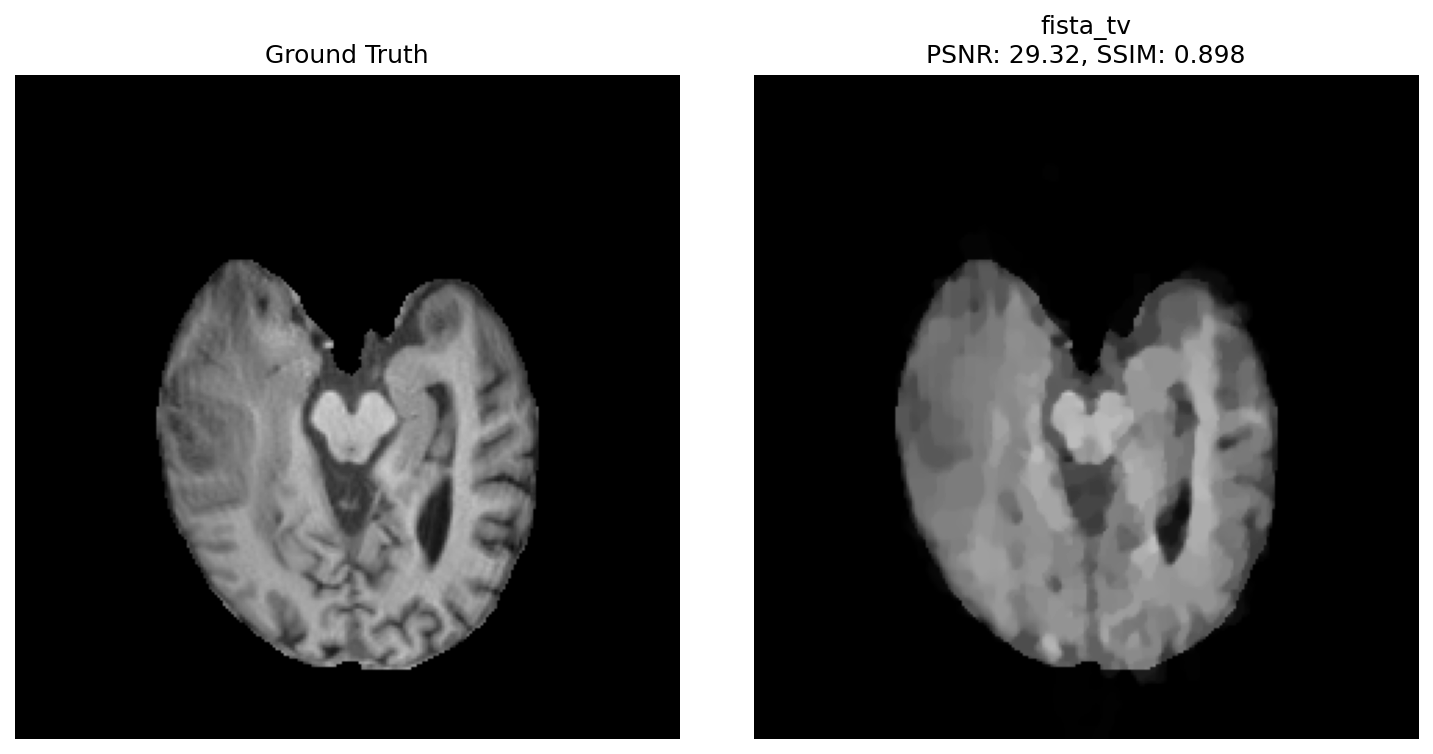
\includegraphics[trim={360pt 0 0 0}, clip,
        width=0.3\linewidth]{figs/fista_tv_batch0000.png} &
        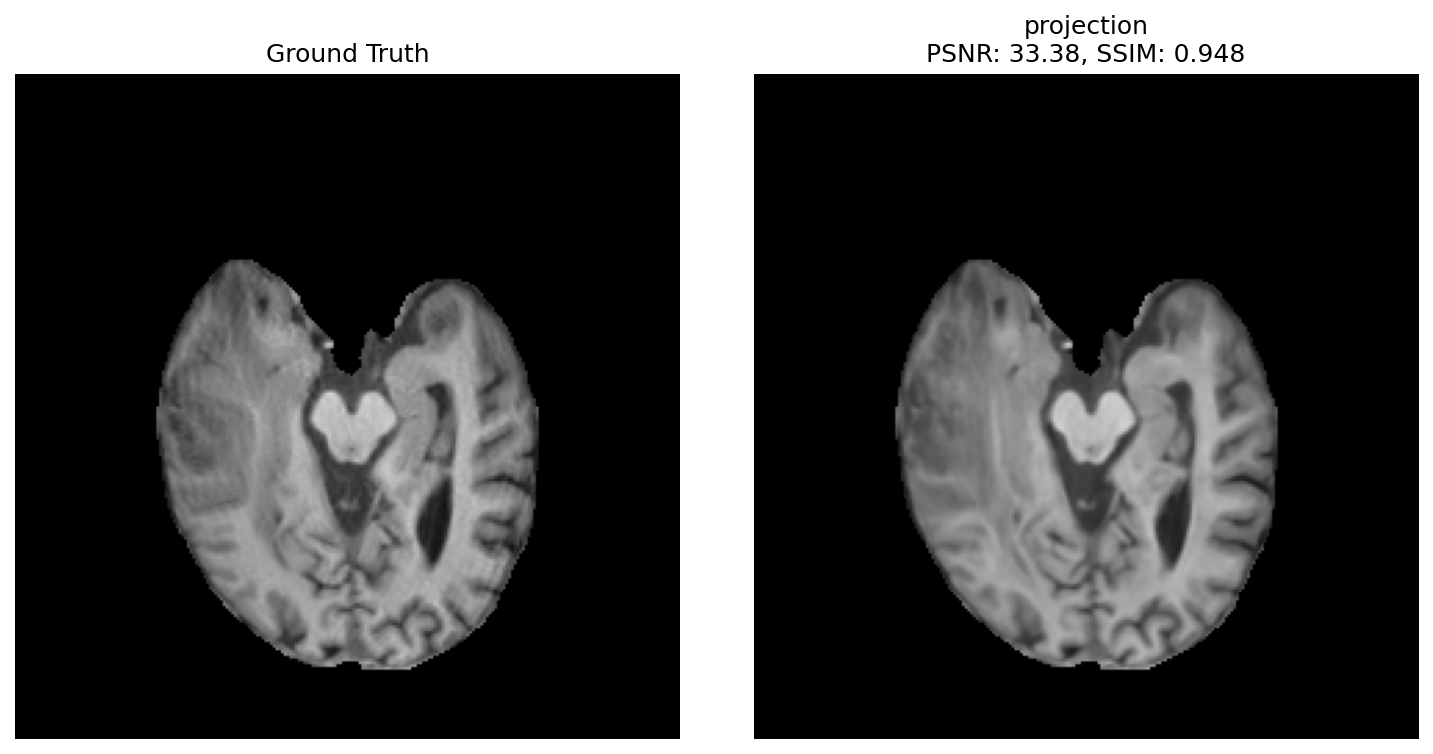
\includegraphics[trim={360pt 0 0 0}, clip,
        width=0.3\linewidth]{figs/projection_batch0000.png} &
        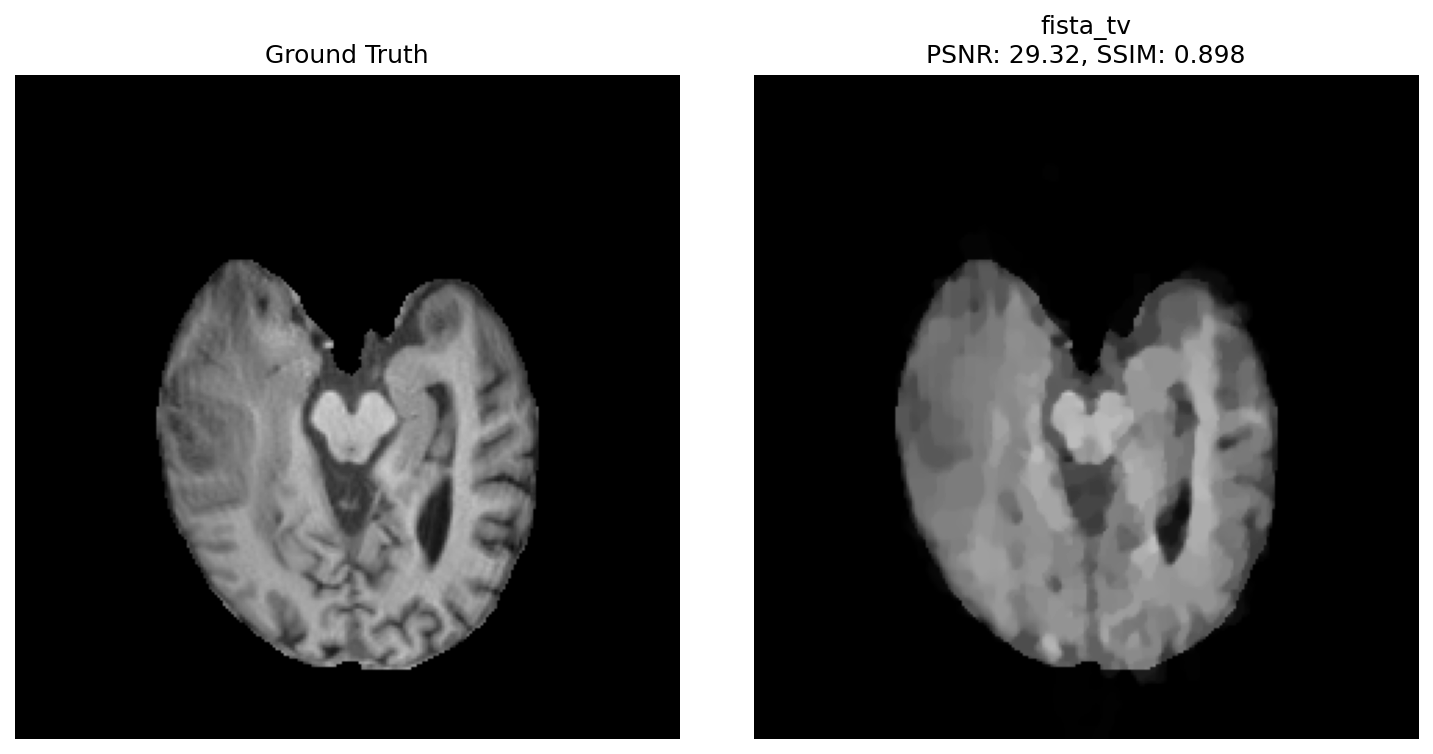
\includegraphics[trim={0 0 360pt 0}, clip,
        width=0.3\linewidth]{figs/fista_tv_batch0000.png} \\[2pt]
        % Row 2 - batch0002
        % 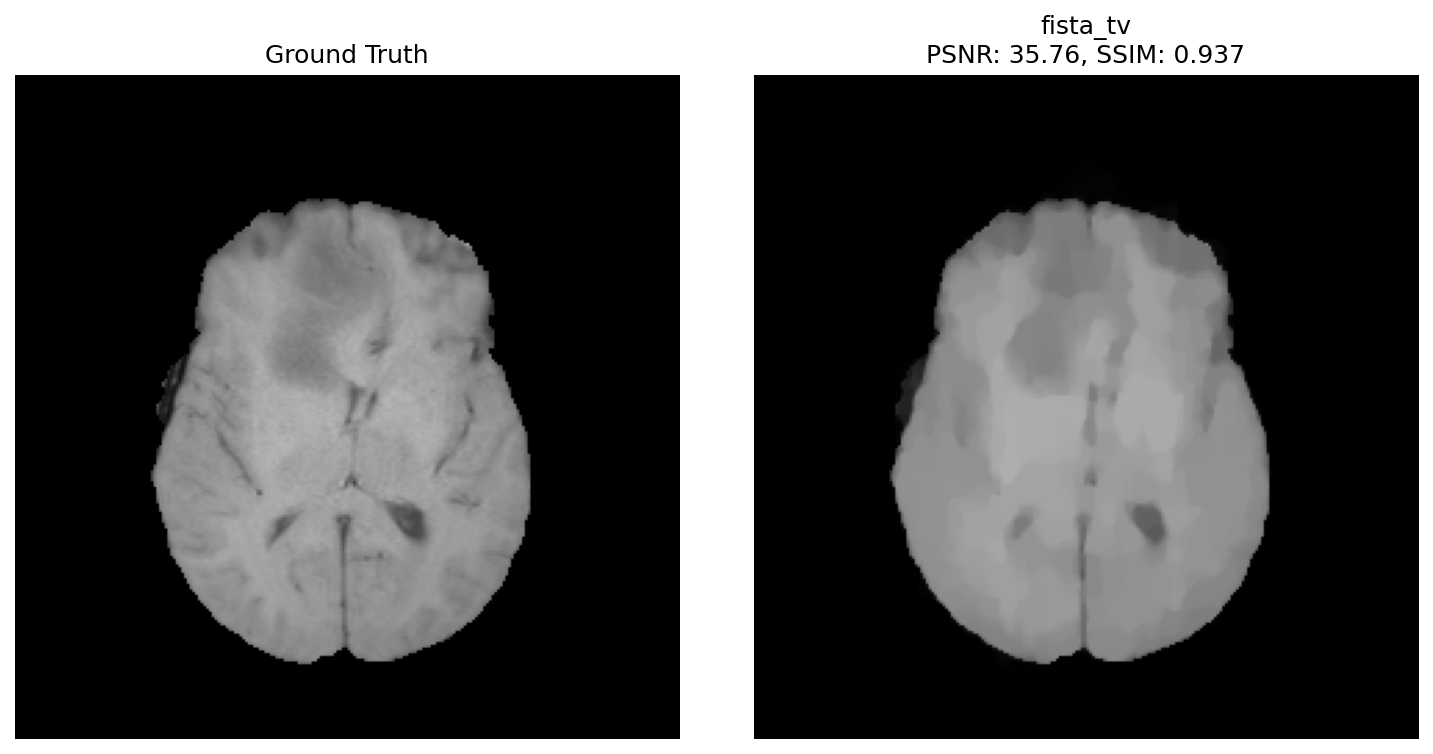
\includegraphics[trim={360pt 0 0 0}, clip,
        % width=0.3\linewidth]{figs/fista_tv_batch0002.png} &
        % 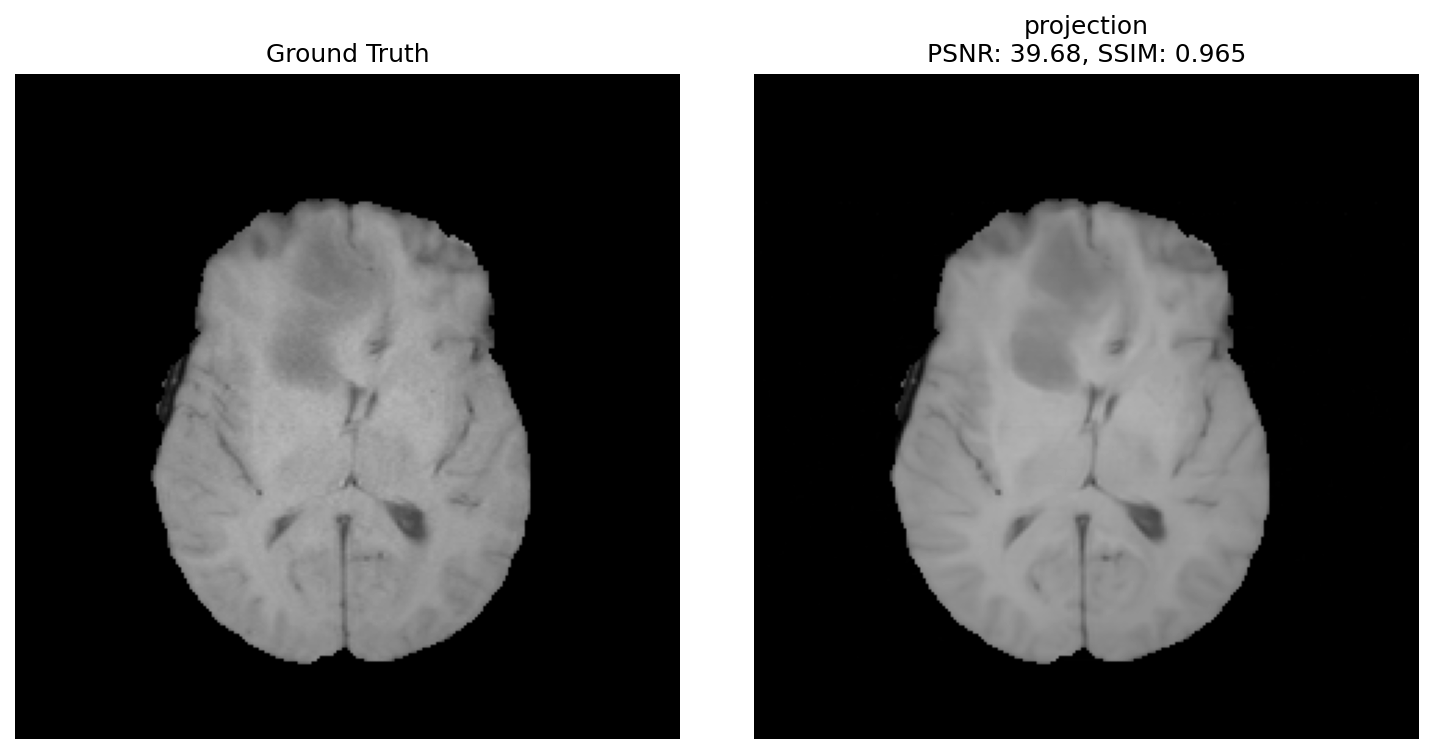
\includegraphics[trim={360pt 0 0 0}, clip,
        % width=0.3\linewidth]{figs/projection_batch0002.png} &
        % 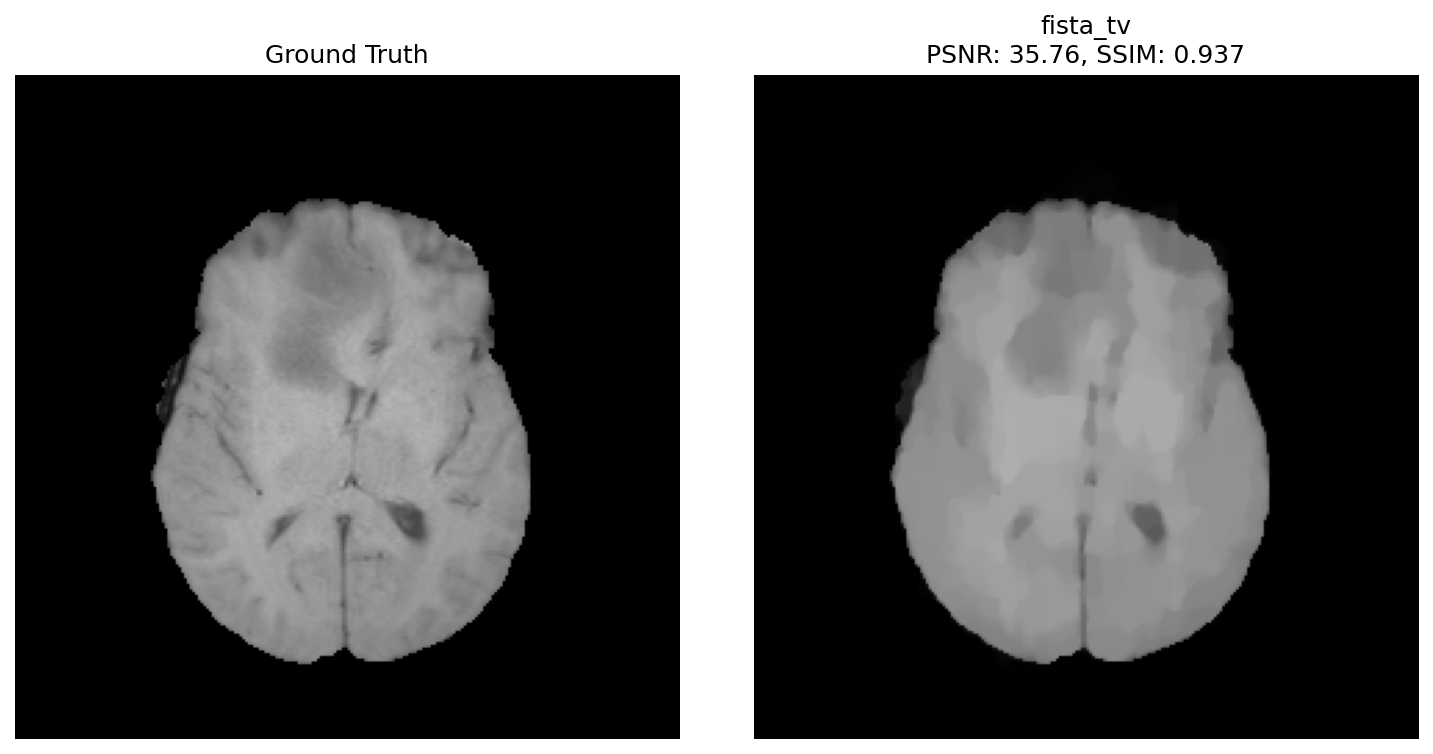
\includegraphics[trim={0 0 360pt 0}, clip,
        % width=0.3\linewidth]{figs/fista_tv_batch0002.png} \\[2pt]
        % Row 3 - batch0006
        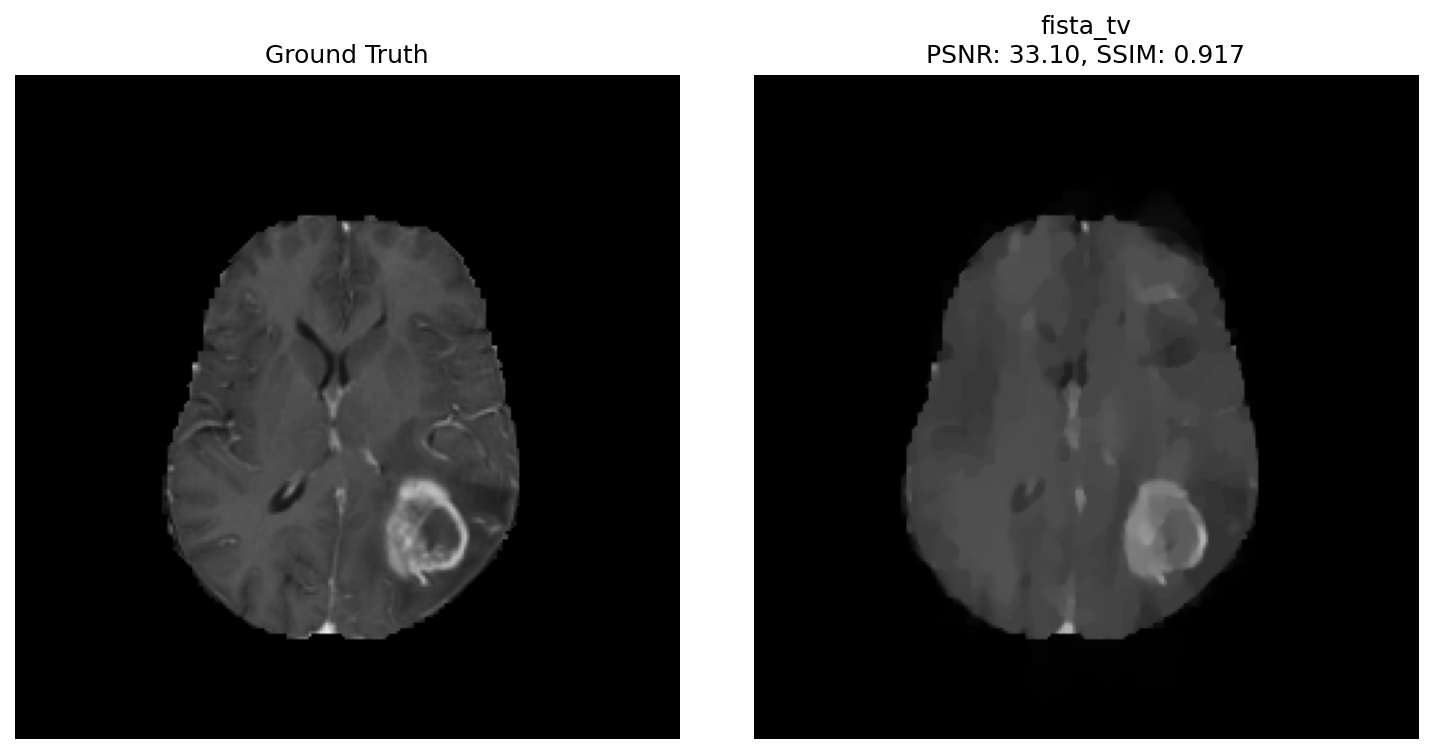
\includegraphics[trim={360pt 0 0 0}, clip,
        width=0.3\linewidth]{figs/fista_tv_batch0006.png} &
        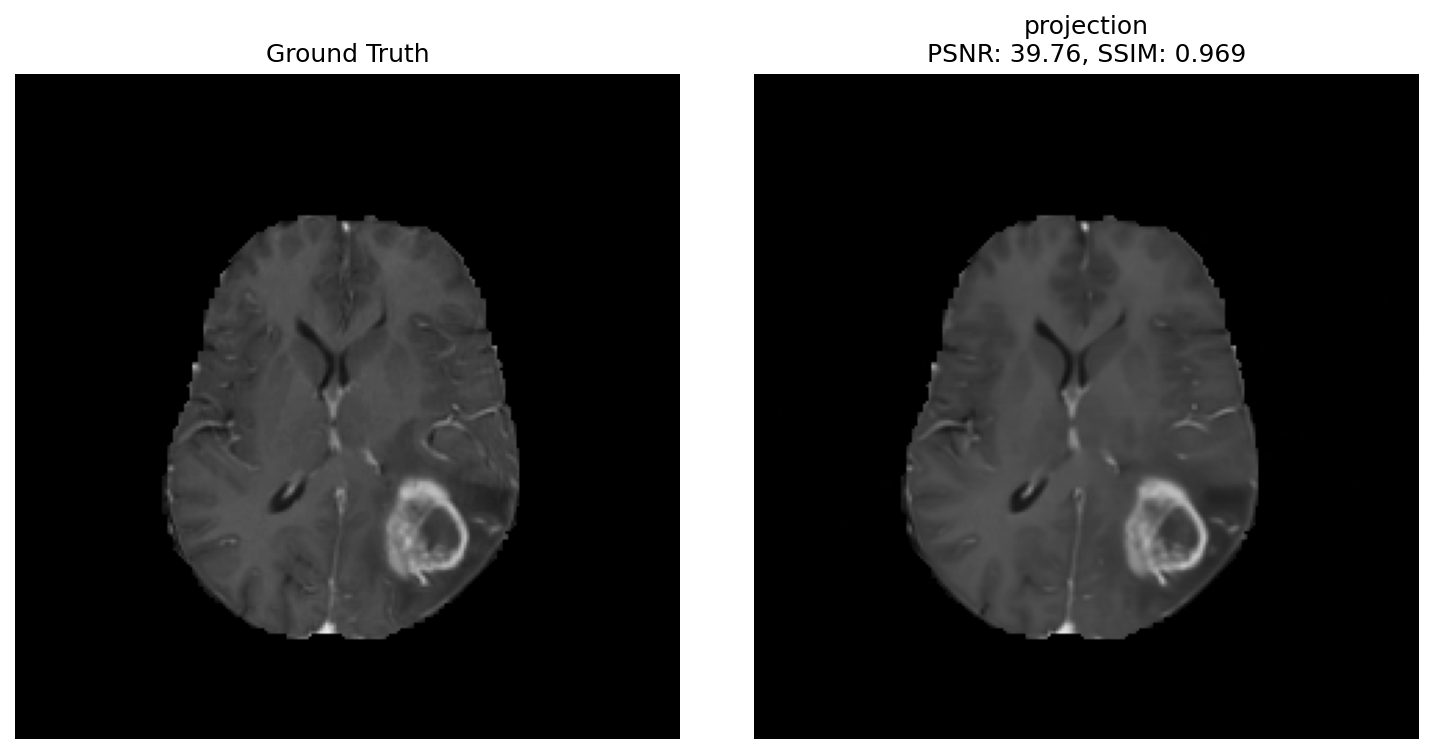
\includegraphics[trim={360pt 0 0 0}, clip,
        width=0.3\linewidth]{figs/projection_batch0006.png} &
        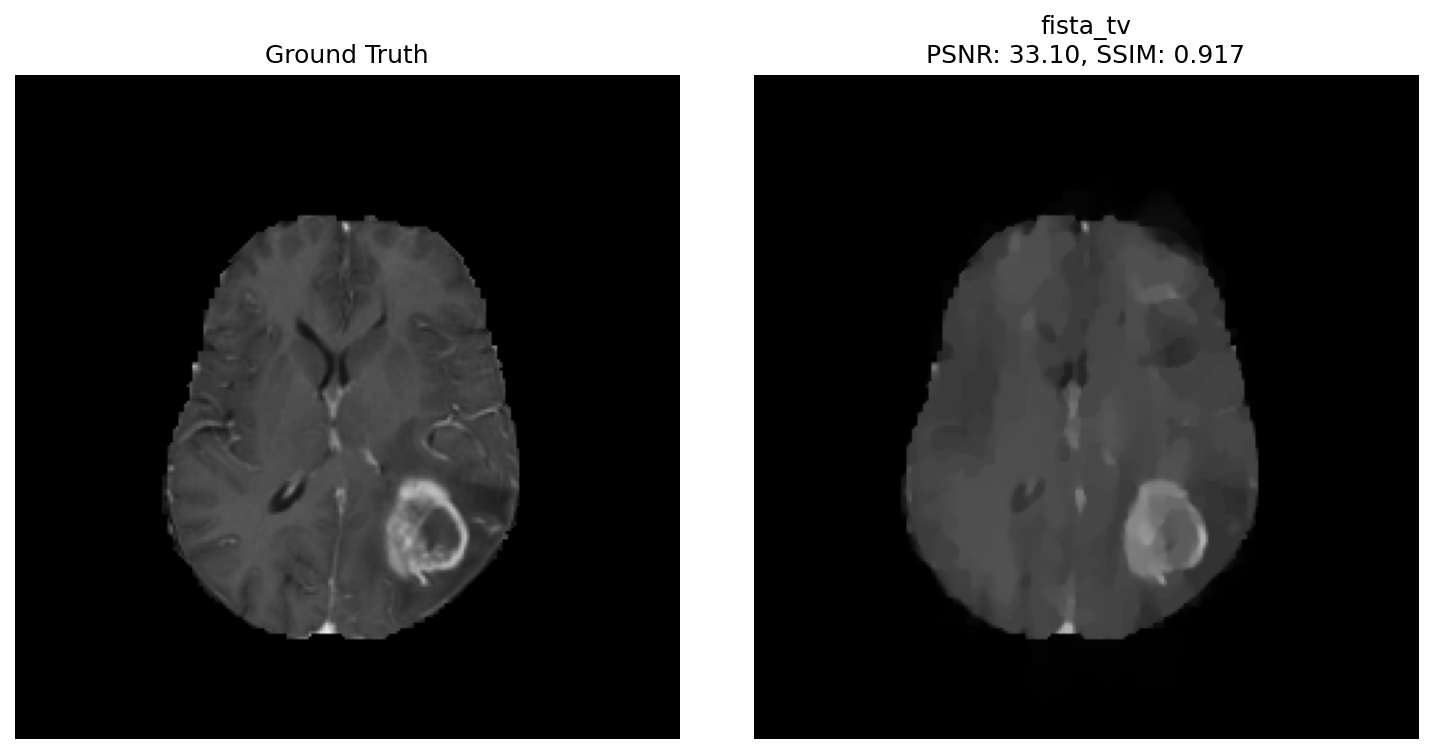
\includegraphics[trim={0 0 360pt 0}, clip,
        width=0.3\linewidth]{figs/fista_tv_batch0006.png}
    \end{tabular}
    \caption{\textbf{Comparación visual de métodos de reconstrucción de resonancia magnética.}
        Tres ejemplos de reconstrucciones de resonancia magnética cerebral que muestran FISTA-TV, el
        enfoque de difusión basado en la consistencia de las mediciones
        de \textcite{song2022solving} e imágenes de referencia
        del conjunto de datos de reconstrucción de resonancia magnética BraTS con un submuestreo de 8x.
        El enfoque basado en la difusión produce reconstrucciones que se
        ajustan mejor a la estructura de la imagen de referencia en comparación con
        FISTA-TV, que, como se puede
        observar, suaviza en exceso los detalles finos presentes en la
        imagen de referencia. Al
        mismo tiempo, el grado de fidelidad a la imagen de referencia
        en la
        reconstrucción basada en la difusión (que surge de la aplicación adecuada de la
    consistencia de las mediciones) es notable.}
    \label{fig:mri-reconstruction-visual}
\end{figure}

\begin{table}[t]
    \centering
    \begin{tabular}{@{}lccc@{}}
        \toprule
        Método & $24\times$ acel. & $8\times$ acel. & $4\times$ acel. \\
        \midrule
        Cascade DenseNet & $23.39_{\pm 2.17}$ & $28.35_{\pm 2.30}$ &
        $30.97_{\pm 2.33}$ \\
        DuDoRNet & $18.46_{\pm 3.05}$ & $\bf 37.88_{\pm 3.03}$ &
        $30.53_{\pm 4.13}$ \\
        \textcite{song2020score} & $27.83_{\pm 2.73}$ & $35.04_{\pm
        2.11}$ & $37.55_{\pm 2.08}$ \\
        \textcite{NEURIPS2021_7d6044e9} & $28.80_{\pm 3.21}$ &
        $36.44_{\pm 2.28}$ & $38.76_{\pm 2.32}$ \\
        \textcite{song2022solving} & $\bf 29.42_{\pm 3.03}$ &
        $37.63_{\pm 2.70}$ & $\bf 39.91_{\pm 2.67}$ \\
        \bottomrule
    \end{tabular}
    \caption{\textbf{Resultados de la reconstrucción de resonancia magnética} en los que se comparan
        enfoques de ajuste de medidas con diferentes factores de aceleración
        (el grado de submuestreo del espacio de Fourier en $\cS$) en el conjunto de datos
        de reconstrucción de resonancia magnética BraTS. Se presentan las métricas PSNR
        (cuanto más alto, mejor) junto con sus desviaciones estándar. Cascade DenseNet
        \cite{NEURIPS2019_1e48c442} y DuDoRNet \cite{9156506} son modelos de referencia supervisados
        entrenados con muestras emparejadas a un nivel de aceleración de 8x.
        Los últimos
        tres métodos son enfoques basados en la difusión que utilizan
        la consistencia de las mediciones.
    Reproducido con permiso de \textcite{song2022solving}.}
    \label{tab:mri-reconstruction}
\end{table}

\section{Inferencia condicional con datos y mediciones emparejados}
\label{sec:paired-data}
En muchas aplicaciones prácticas, no conocemos ni la
distribución de los datos $\x$ de interés ni la relación explícita
entre los datos y ciertos atributos observados $\y$ de
los datos. Solo tenemos un conjunto (grande) de muestras emparejadas $(\X, \Y) =
\{ (\x_1, \y_1), \ldots, (\x_N, \y_N) \}$ a partir del cual necesitamos inferir
la distribución de los datos y una correspondencia que modele su relación:
\begin{equation}
    h: \x \mapsto \y.
\end{equation}

El problema de la clasificación de imágenes puede considerarse un ejemplo de ello.
En cierto sentido, el problema de la clasificación consiste en aprender un
codificador compresivo (con una pérdida de información extremadamente elevada) para imágenes naturales. Digamos que, dada
una muestra aleatoria de una imagen $\x$, nos gustaría predecir su etiqueta de clase
$\y$ que mejor se correlacione con el contenido de $\x$. Sabemos que la
distribución de las imágenes naturales de los objetos es de baja dimensión en comparación
con la dimensión del espacio de píxeles. En los capítulos anteriores,
hemos aprendido que, si contamos con suficientes muestras, en principio podemos
aprender una representación estructurada de baja dimensión $\z$ para $\x$
mediante una codificación compresiva aprendida:
\begin{equation}
    f: \x \mapsto \z.
\end{equation}
La representación $\z$ también puede considerarse como un código aprendido (con pérdida, pero
estructurado) para $\x$. Es bastante razonable suponer que si
la asignación de clase $\y$ depende realmente de las estructuras de baja dimensión
de $\x$ y el código aprendido $\z$ refleja realmente dichas
estructuras, $\y$ y $\z$ pueden hacerse altamente correlacionadas y, por lo tanto,
su distribución conjunta $p(\z, \y)$ debería ser de dimensión extremadamente
baja. Por lo tanto, podemos combinar los dos códigos deseados, $\y$
y $\z$ e intentar entrenar un codificador combinado: 
\begin{equation}
    f: \x \mapsto (\z, \y)
\end{equation}
donde la distribución conjunta de $(\z, \y)$ es de muy baja dimensión.

Según lo visto en los capítulos anteriores, el mapeo $f$ suele
aprenderse como una secuencia de operadores de compresión o de eliminación de ruido en el
mismo espacio. Por lo tanto, para aprovechar esta familia de operaciones, podemos
introducir un vector auxiliar $\vw$ que puede considerarse como una
conjetura aleatoria inicial de la etiqueta de clase $\y$. De esta manera, podemos aprender un
mapeo de compresión o de eliminación de ruido:
\begin{equation}\label{eq:classifier-with-class-token}
    f: (\x, \vw) \mapsto (\z, \y)
\end{equation}
dentro de un espacio común. De hecho, la práctica habitual de introducir un
«token de clase» auxiliar en el entrenamiento de un transformador para
tareas de clasificación, como en ViT, puede considerarse como el aprendizaje de dicha
representación mediante la compresión (de la tasa de codificación de) muestras dadas (con ruido)
de $(\x, \vw)$. Si la distribución de los datos $\x$ es
ya una mezcla de gaussianas (de baja dimensión), el trabajo
\cite{wright2008classification} ha demostrado que la clasificación puede
realizarse de manera eficaz minimizando directamente {\em la longitud de codificación 
(con pérdida)} asociada a las muestras dadas.

\subsection{Generación de imágenes condicionada por clases}\label{sub:cfg}
Si bien un clasificador entrenado nos permite clasificar una imagen dada $\x$ en su
clase correspondiente, a menudo nos interesa generar una imagen de una
clase determinada, mediante
el muestreo de la distribución aprendida de imágenes naturales. En cierta medida, esto puede
considerarse como el problema «inverso» a la clasificación de imágenes. Sea $p_{\x}$ la
distribución de imágenes naturales, modeladas, por ejemplo, mediante un proceso de
eliminación de ruido por difusión. Dada una variable aleatoria de clase $y \in [K]$ con
realización $\nu$, por ejemplo,
una «Manzana», nos gustaría muestrear la distribución condicional $p_{\x \mid
y}(\,\cdot\, \mid \nu)$ para generar una imagen de una manzana:
\begin{equation}
    \hat{\x} \sim p_{\x\mid \y}(\,\cdot\, \mid \vnu).
\end{equation}
A esto lo llamamos «generación de imágenes condicionada por la clase».

En la \Cref{sec:conditioned-decoding}, hemos visto cómo utilizar el
paradigma de difusión con eliminación de ruido para el
muestreo condicional a partir de la distribución a posteriori $p_{\vx \mid \vy}$ dada
una medición \textit{basada en el modelo} $\vy = h(\vx) + \vw$
(\Cref{eq:measurement-matching-observation}), lo que culmina en el
algoritmo DPS (\Cref{alg:iterative_denoising_conditional_DPS}). Este
es un marco
potente, pero no se aplica al problema de la generación de imágenes condicionadas por clase (o texto)
que nos ocupa, en el que no se dispone de un modelo generativo explícito $h$ para las
observaciones/atributos $y$ debido a lo
inmanejable de la modelación analítica. En esta sección,
presentaremos técnicas para extender
el muestreo condicional a este contexto.

Por lo tanto, ahora suponemos únicamente que tenemos acceso a muestras de la distribución conjunta
de $(\vx, y)$:
\begin{equation}
    (\vx, y) \sim p_{\vx, y}.
\end{equation}
Al igual que en la sección anterior, definimos $\vx_t = \alpha_t \vx + \sigma_t \vg$
donde $\vg \sim \cN(\Zero, \vI)$ es independiente de $(\vx, \vy)$, tal como se muestra en la
\Cref{eq:gen_additive_gaussian_noise_model} del \Cref{ch:denoising},
y utilizaremos repetidamente la notación $\vxi$ para denotar realizaciones de $\vx$
y $\vx_t$.

Esta sección se centra en los fundamentos conceptuales y algorítmicos del
muestreo condicional en los modelos generativos modernos. Para un análisis centrado en
las cuestiones de implementación en diversas aplicaciones, véanse el \Cref{ch:applications},
\Cref{sec:cond_gen} y las secciones siguientes.

\subsubsection{Guía de clasificadores: consistencia mediante un clasificador preentrenado}

% To proceed, we note that our development of conditional sampling under
% measurements $\vy = h(\vx) + \vw$ only explicitly used the
% forward model $h$ in making the DPS approximation
% \eqref{eq:conditional-posterior-measurementmatching-gaussian-case-dps-approx}.
Recordemos de la \Cref{sec:conditioned-decoding}
que se cumple la siguiente descomposición del filtro de ruido posterior condicional óptimo:
% In particular, the conditional posterior denoiser decomposition
% \eqref{eq:posterior-sampling-denoiser-decomposition} \textit{still
% holds in the
% paired data setting},
en virtud de la regla de Bayes
y de la independencia condicional de $\vy$ y $\vx_t$ dado $\vx$ (véase la
\Cref{fig:posterior-sampling-cds}):
\begin{equation}\label{eq:conditional-denoising-mmse-denoiser-paired-data}
    \bE[ \vx \mid \vx_t=\vxi, y=\nu]
    =
    \bE[\vx \mid \vx_t=\vxi]
    + \frac{\sigma_t^2}{\alpha_t}
    \nabla_{\vxi}\log p_{y \mid \vx_t}(\nu\mid \vxi).
\end{equation}
En otras palabras, la representación
\eqref{eq:conditional-denoising-mmse-denoiser-paired-data}
del filtro de ruido condicional óptimo se mantiene independientemente de si el modelo de observación explícito
$\vy = h(\vx) + \vw$ es válido.
Esto significa que, si logramos aprender un filtro de ruido de este tipo
\eqref{eq:conditional-denoising-mmse-denoiser-paired-data} en el contexto de datos emparejados,
podremos seguir la metodología de difusión con eliminación de ruido que hemos desarrollado en el
\Cref{ch:denoising} para realizar un muestreo condicional por clase.

Una idea lógica es, entonces, implementar directamente el término de corrección de verosimilitud en
\eqref{eq:conditional-denoising-mmse-denoiser-paired-data} utilizando una red profunda
$f_{\theta_{\mathrm{c}}}$ con parámetros $\theta_{\mathrm{c}}$, tal como se muestra en
\Cref{eq:classifier-with-class-token}:
\begin{equation}
    f_{\theta_{\mathrm{c}}} : (t, \vx_t) \mapsto \softmax(\vW_{\mathrm{head}}
    \vz(t, \vx_t)).
\end{equation}
Esta expresión combina las representaciones finales $\vz(t, \vx_t)$
(que también dependen de
$\theta_{\mathrm{c}}$) de las entradas con ruido
$\vx_t$ con un cabezal de clasificación $\vW_{\mathrm{head}} \in \bR^{K
\times d}$, que mapea las
representaciones a una distribución de probabilidad sobre las $K$ clases posibles.
Como es habitual en la práctica, también toma el tiempo $t$ en el proceso de ruido como
entrada.
Por lo tanto, con un entrenamiento adecuado, proporciona una aproximación a la
verosimilitud logarítmica
$\log p_{y \mid \vx_t}$, y la derivación de $\log f_{\theta_{\mathrm{c}}}$
respecto a su entrada $\vx_t$
permite una aproximación al segundo término de
\Cref{eq:conditional-denoising-mmse-denoiser-paired-data}:
\begin{equation}\label{eq:conditional-denoising-mmse-denoiser-paired-data-approx}
    \bar{\vx}_{\theta}^{\mathrm{naive}}(t, \vx_t, y)
    =
    \bar{\vx}_{\theta_{\mathrm{d}}}(t, \vx_t)
    + \frac{\sigma_t^2}{\alpha_t}
    \nabla_{\vx_t}
    \ip*{
        \log f_{\theta_{\mathrm{c}}}(t, \vx_t)
    }{
        \ve_{y}
    }
\end{equation}
donde, como es habitual, aproximamos el primer término de
\Cref{eq:conditional-denoising-mmse-denoiser-paired-data} mediante un
filtro de ruido incondicional aprendido para $\vx_t$ con parámetros $\theta_{\mathrm{d}}$ y
donde escribimos $\ve_k$ para $k \in [K]$ para denotar el $k$-ésimo vector de base canónica
para $\R^K$ (es decir, el vector con
un uno en la posición $k$-ésima, y ceros en el resto).
El lector debe tener en cuenta que el filtro de ruido condicional $\bar{\vx}_{\theta}$
requiere dos procesos de entrenamiento independientes, con pérdidas distintas: uno para los
parámetros del clasificador $\theta_{\mathrm{c}}$, sobre una pérdida de clasificación
\footnote{En \Cref{ch:applications}, revisamos el proceso de entrenamiento de dicho
clasificador con todo detalle.} y otro para los parámetros del filtro de ruido
$\theta_{\mathrm{d}}$, sobre una pérdida de eliminación de ruido. Este enfoque del muestreo condicional
ya se había reconocido y aprovechado para llevar a cabo el muestreo condicional en
los primeros trabajos pioneros sobre modelos de difusión, en particular los de
\citet{Sohl-Dickstein2015} y \citet{song2020score}. 

Sin embargo, esta metodología sencilla presenta dos inconvenientes fundamentales (razón por la cual
la calificamos de «ingenua»). El primero es
que, según la experiencia, un clasificador de red profunda entrenado de este modo a menudo no
proporciona una señal de orientación lo suficientemente sólida (en la
\Cref{eq:conditional-denoising-mmse-denoiser-paired-data}) como para garantizar que
las muestras generadas reflejen la información de condicionamiento $y$. Esto fue destacado por primera vez
por \citet{Dhariwal2021-hg}, quien señaló que, en el contexto de la
generación de ImageNet condicionada por clase, las probabilidades
de salida del clasificador de red profunda entrenado para la clase $y$ sobre la que se
aplicaba la condición solían rondar
$0,5$---lo suficientemente grande como para ser la clase dominante, pero no lo suficiente como para proporcionar
una señal de orientación sólida---y que, tras su inspección, las generaciones no eran
consistentes con la clase de condicionamiento $y$. \citet{Dhariwal2021-hg} propuso
abordar esto de manera heurística incorporando un hiperparámetro de «temperatura inversa»
$\gamma > 0$
en la definición del filtro de ruido condicional ingenuo
\eqref{eq:conditional-denoising-mmse-denoiser-paired-data-approx},
refiriéndose al
filtro de ruido condicional resultante como si hubiera incorporado 
\textbf{«orientación del clasificador»} (CG):
\begin{equation}\label{eq:conditional-denoising-mmse-denoiser-paired-data-approx-cg}
    \bar{\vx}_{\theta}^{\mathrm{CG}}(t, \vx_t, y)
    =
    \bar{\vx}_{\theta_{\mathrm{d}}}(t, \vx_t)
    + \gamma\frac{\sigma_t^2}{\alpha_t}
    \nabla_{\vx_t}
    \ip*{
        \log f_{\theta_{\mathrm{c}}}(t, \vx_t)
    }{
        \ve_{y}
    }
\end{equation}
que en el caso en que $\gamma = 1$ coincide con
\eqref{eq:conditional-denoising-mmse-denoiser-paired-data-approx}.

\citet{Dhariwal2021-hg} descubrió que un valor de $\gamma > 1$ ofrecía
los mejores resultados empíricos.
Una posible interpretación de esto es la siguiente: obsérvese que, en el contexto del
término de verosimilitud \textit{verdadera}
\Cref{eq:conditional-denoising-mmse-denoiser-paired-data}, la multiplicación por $\gamma$
da como resultado, de manera equivalente,
\begin{align}
    \gamma\frac{\sigma_t^2}{\alpha_t} \nabla_{\vxi}\log p_{\vy \mid
    \vx_t}(\vnu\mid
    \vxi)
    &=
    \frac{\sigma_t^2}{\alpha_t} \nabla_{\vxi}\log \left(
        p_{\vy \mid \vx_t}(\vnu\mid \vxi)^\gamma
    \right), %
\end{align}
lo que sugiere la interpretación natural de que el parámetro $\gamma$ realiza
un \textit{escalado de temperatura} (inverso) sobre la verosimilitud
$p_{\vy \mid \vx_t}$, lo cual es exacto si consideramos la distribución
renormalizada
$ { p_{\vy \mid \vx_t}(\vnu\mid \vxi)^\gamma } / { \int p_{\vy \mid
    \vx_t}(\vnu'\mid
\vxi)^\gamma \odif \vnu' } $
Sin embargo, cabe señalar que esta \textit{no es} una interpretación rigurosa en el contexto
de \Cref{eq:conditional-denoising-mmse-denoiser-paired-data}, ya que los
gradientes se calculan con respecto a $\vxi$ y la constante de normalización en
la distribución escalada por temperatura es, en general, una función de $\vxi$.
En cambio, el parámetro $\gamma$ debe entenderse simplemente como una amplificación de los
valores altos de las probabilidades de salida del clasificador de red profunda
$f_{\theta_{\mathrm{c}}}(t, \vx_t)$ \textit{en relación con} los más bajos,
lo que amplifica efectivamente la señal de orientación proporcionada en los casos en que la red profunda
$f$ le asigna la probabilidad más alta entre las $K$ clases.

\subsubsection{Simplificaciones y mejoras mediante la orientación sin clasificadores}

No obstante, la orientación mediante clasificador no resuelve el segundo inconveniente clave de
la metodología ingenua: resulta engorroso y poco eficiente tener que
entrenar un clasificador auxiliar $f_{\theta_{\mathrm{c}}}$ además
del filtro de ruido incondicional
$\bar{\vx}_{\theta_{\mathrm{d}}}$, dado
que no es posible adaptar directamente un clasificador preentrenado
debido a la necesidad de que funcione bien con entradas ruidosas $\vx_t$ e incorpore
otras modificaciones de arquitectura motivadas empíricamente.
En concreto, \citet{Dhariwal2021-hg} descubrió que era necesario
\textit{diseñar explícitamente
    la arquitectura de la red profunda que implementa el
    clasificador para que coincida
con la del filtro de ruido}.

Además, desde una perspectiva puramente práctica---es decir, al intentar obtener el mejor
rendimiento posible del muestreador resultante, la configuración más eficaz
del muestreo basado en la orientación del clasificador se aleja aún más del
marco idealizado y conceptualmente sólido que hemos presentado anteriormente.
Para obtener el mejor rendimiento, \citet{Dhariwal2021-hg} consideró
necesario proporcionar la etiqueta de clase $y$ como una entrada adicional al filtro de ruido
$\bar{\vx}_{\theta_{\mathrm{d}}}$. Como resultado, el eliminador de ruido idealizado guiado por un clasificador
\eqref{eq:conditional-denoising-mmse-denoiser-paired-data-approx-cg},
derivado por \citet{Dhariwal2021-hg} tal y como hemos hecho anteriormente a partir de la descomposición
condicional del eliminador de ruido posterior
\eqref{eq:conditional-denoising-mmse-denoiser-paired-data}, no refleja exactamente
el denoiser de mejor rendimiento en la práctica; ¡dicho filtro de ruido
combina en realidad un filtro de ruido \textit{condicional} para $\vx_t$ dado $y$ con una
señal de guía adicional procedente de un clasificador auxiliar!

Esta situación, de carácter empírico, llevó a \citet{Ho2022-ry} en
trabajos posteriores a proponer una metodología más pragmática desde el punto de vista empírico, conocida como
\textbf{orientación sin clasificador (CFG)}. En lugar de representar el
denoiser condicional
\eqref{eq:conditional-denoising-mmse-denoiser-paired-data} como una suma ponderada
de un denoiser incondicional para $\vx_t$ con un término de corrección de la verosimilitud logarítmica
(con pesos posiblemente modificados, como en la guía del clasificador), aceptan la
aparente necesidad de entrenar un denoiser condicional para $\vx_t$ dado $y$, tal como
lo demuestran los resultados experimentales de \citet{Dhariwal2021-hg}, y sustituir
el término del gradiente de la verosimilitud logarítmica por una suma correctamente ponderada de este
denoiser condicional con un denoiser \textit{incondicional} para $\vx$ dado
$\vx_t$.\footnote{Dicho esto, \textcite{Ho2022-ry} propuso en realidad utilizar
    una ponderación diferente a la que presentamos aquí, basándose en el hecho de que
    \textcite{Dhariwal2021-hg} sustituyó de forma heurística el
    denoiser incondicional de 
    \eqref{eq:conditional-denoising-mmse-denoiser-paired-data} por
    un denoiser condicional. De hecho, la ponderación que derivamos y presentamos aquí
    refleja la práctica moderna y, en particular, se utiliza en modelos de difusión de vanguardia
    como Stable Diffusion 3.5 
\cite{DBLP:conf/icml/EsserKBEMSLLSBP24}.}

\paragraph{Derivación de la orientación sin clasificador.} Para ver cómo surge esta
estructura, comenzamos con una versión «idealizada» del filtro de ruido con guía de clasificador
$\bar{\vx}_{\theta}^{\mathrm{CG}}$ definido en la
\eqref{eq:conditional-denoising-mmse-denoiser-paired-data-approx-cg},
para el cual el filtro de ruido $\bar{\vx}_{\theta_{\mathrm{d}}}$ y el clasificador
$f_{\theta_{\mathrm{c}}}$ se aproximan perfectamente a sus objetivos, mediante
\eqref{eq:conditional-denoising-mmse-denoiser-paired-data}:
\begin{equation}\label{eq:conditional-denoising-mmse-denoiser-paired-data-exact-cg}
    \bar{\vx}_{\theta}^{\mathrm{CG,\,ideal}}(t, \vxi, \nu)
    =
    \bE[\vx \mid \vx_t=\vxi]
    + \gamma\frac{\sigma_t^2}{\alpha_t}
    \nabla_{\vxi}\log p_{y \mid \vx_t}(\nu\mid \vxi).
\end{equation}
A continuación, utilizamos la regla de Bayes, en la forma
\begin{equation}
    \log p_{y \mid \vx_t}
    =
    \log p_{\vx_t \mid y} + \log p_{y} - \log p_{\vx_t},
\end{equation}
junto con la fórmula de Tweedie (\Cref{thm:tweedie}, modificada como en
\Cref{eq:gen_tweedie}) para convertir entre funciones de puntuación y filtros de ruido,
a fin de obtener
\begin{align*}
    \bar{\vx}_{\theta}^{\mathrm{CG,\,ideal}}(t, \vxi, \nu)
    &=
    \frac{1}{\alpha_t} \vxi
    + (1-\gamma) \frac{\sigma_t^2}{\alpha_t}
    \nabla_{\vxi}\log p_{\vx_t}(\vxi)
    + \gamma \frac{\sigma_t^2}{\alpha_t}
    \nabla_{\vxi}\log p_{\vx_t \mid y}(\vxi \mid \nu)
    \\
    &=
    (1 - \gamma) \bE[\vx \mid \vx_t=\vxi]
    +
    \gamma \bE[\vx \mid \vx_t=\vxi, y=\nu],
    \labelthis\label{eq:ideal-cfg-denoiser}
\end{align*}
donde, en la última línea, aplicamos la
\Cref{eq:conditional-denoising-conditioning-order-irrelevant}.
Ahora, la \Cref{eq:ideal-cfg-denoiser} sugiere una estrategia de aproximación natural:
combinamos un filtro de ruido incondicional aprendido para $\vx$ dado $\vx_t$, como antes,
con un filtro de ruido \textit{condicional} aprendido para $\vx$ dado $\vx_t$ y $y$.

Sin embargo, siguiendo a \textcite{Ho2022-ry} y la práctica habitual en el
entrenamiento de filtro de ruido de redes profundas,
lo habitual es utilizar la \textit{misma} red profunda para representar
tanto el filtro de ruido condicional como el incondicional mediante la introducción de una
etiqueta adicional, que denotaremos como $\varnothing$, para indicar el caso «incondicional».
Esto da lugar a la forma del denoiser CFG:
\begin{equation}\label{eq:conditional-denoising-mmse-denoiser-paired-data-approx-cfg}
    \bar{\vx}_{\theta}^{\mathrm{CFG}}(t, \vx_t, y)
    =
    (1 - \gamma) \bar{\vx}_{\theta}(t, \vx_t, \varnothing)
    +
    \gamma \bar{\vx}_{\theta}(t, \vx_t, y).
\end{equation}
Para entrenar un denoiser $\bar{\vx}_{\theta}(t, \vx_t, y^+)$ destinado a
el muestreo de orientación sin clasificador, donde $y^+ \in
\set{1, \dots, K, \varnothing}$, procedemos de manera casi idéntica al
procedimiento de entrenamiento incondicional descrito en \Cref{alg:learning_denoiser}, pero con dos
modificaciones:
\begin{enumerate}
    \item Cuando tomamos muestras del conjunto de datos, tomamos un par $(\vx, y)$ en lugar de
        solo una muestra $\vx$.
    \item Cada vez que extraemos un par del conjunto de datos, obtenemos la etiqueta aumentada
        $y^+$ mediante
        \begin{equation}
            y^+ =
            \begin{cases}
                \varnothing & \text{with probability } p_{\mathrm{uncond}}; \\
                y & \text{else}.
            \end{cases}
        \end{equation}
        Aquí, $p_{\mathrm{uncond}} \in [0, 1]$ es un nuevo hiperparámetro.
        Esto puede considerarse una forma de dropout \cite{srivastava2014dropout}.
\end{enumerate}
De esta manera, entrenamos un filtro de ruido condicional adecuado para su uso en el muestreo guiado sin clasificador.
Resumimos el proceso general de muestreo para
el muestreo condicionado por clase con guía sin clasificador en
\Cref{alg:iterative_denoising_conditional_CFG}.

\begin{algorithm}
    \caption{Muestreo condicional con datos de clasificación, utilizando
    un filtro de eliminación de ruido condicionado por clase.}
    \label{alg:iterative_denoising_conditional_CFG}
    \begin{algorithmic}[1]
        \Require{Una lista ordenada de intervalos de tiempo \(0 \leq t_{0} < \cdots
        < t_{L} \leq T\) que se utilizarán para el muestreo.}
        \Require{Etiqueta de clase $\nu \in \{1, \dots, K\}$ sobre la que se va a realizar la condición.}
        \Require{Un filtro de ruido \(\bar{\vx}_{\theta} \colon
                \{t_{\ell}\}_{\ell = 1}^{L} \times \R^{D} \times
                \set{1, \dots, K,
            \varnothing} \to \R^{D}\) para $p_{\vx \mid y}$ y
            $p_{\vx}$ (entrada $\varnothing$ para
        $p_{\vx}$).}
        \Require{Funciones de escala y nivel de ruido \(\alpha, \sigma
        \colon \{t_{\ell}\}_{\ell = 0}^{L} \to \R_{\geq 0}\).}
        \Require{Fuerza de orientación $\gamma \geq 0$ (se recomienda $\gamma > 1$ para
        un mejor rendimiento).}
        \Ensure{Una muestra \(\hat{\vx}\), aproximadamente de \(p_{\vx
                \mid y}(\,\cdot\,
        \mid \nu)\).}
        \Function{DDIMSamplerConditionalCFG}{$\bar{\vx}_{\theta}, \nu, \gamma,
        (t_{\ell})_{\ell = 0}^{L}$}
        \State{Initializar \(\hat{\vx}_{t_{L}} \sim\) distribución
            aproximada de \(\vx_{t_{L}}\) (VP \(\implies
        \dNorm(\vzero, \vI)\), VE \(\implies \dNorm(\vzero, t_{L}^{2}\vI)\)).}
        \For{\(\ell = L, L - 1, \dots, 1\)}
        \State{Calcular
            \begin{equation*}
                \hat{\vx}_{t_{\ell - 1}} \doteq \frac{\sigma_{t_{\ell
                - 1}}}{\sigma_{t_{\ell}}}\hat{\vx}_{t_{\ell}} +
                \bp{\alpha_{t_{\ell
                    - 1}} - \frac{\sigma_{t_{\ell
                - 1}}}{\sigma_{t_{\ell}}}\alpha_{t_{\ell}}}\bigl(
                    (1 - \gamma) \bar{\vx}_{\theta}(t_{\ell},
                    \hat{\vx}_{t_{\ell}}, \varnothing)
                    + \gamma \bar{\vx}_{\theta}(t_{\ell},
                    \hat{\vx}_{t_{\ell}}, \nu)
                \bigr)
            \end{equation*}
        }
        \EndFor
        \State{\Return{\(\hat{\vx}_{t_{0}}\)}}
        \EndFunction
    \end{algorithmic}
\end{algorithm}

\textcite{Ho2022-ry} presenta unos sólidos rendimientos empíricos en la generación de imágenes condicionadas por clase
con orientación sin clasificador, y se ha convertido en un pilar fundamental de
los modelos de difusión prácticos a mayor escala, como Stable Diffusion
\cite{rombach2022high} y sus derivados.

\paragraph{¿Qué filtros de ruido promueve aprender la orientación sin clasificador?}
Como hemos visto, la derivación de la orientación sin clasificador es bastante opaca y
se basa en la experiencia,
lo que ofrece poca información sobre los mecanismos que subyacen a su excelente rendimiento.
Varios trabajos teóricos han intentado abordar esta cuestión
\cite{Bradley2024-jg,Li2025-li,Wu2024-js}.
Ofrecen explicaciones sobre algunos aspectos de la metodología general de CFG,
que abarca la parametrización y el entrenamiento del denoiser,
así como la configuración de la intensidad de la guía
y el rendimiento en el momento del muestreo.
A continuación, siguiendo el hilo conductor del libro, daremos una interpretación
en el marco simplificado de una distribución de datos de modelo de mezcla gaussiana y
un denoiser.
En primer lugar, consideramos \textit{el efecto de CFG}: ¿qué promueve un peso grande $\gamma
\gg 1$?

% \yima{Please make messages that the example below try to convey some
% what more modular. Probably break it into two related parts?}
\begin{example}\label{example:denoising-gaussian-mixture-cfg}
    Recordemos el proceso generador de datos de mezcla gaussiana de rango bajo
    que estudiamos en el
    \Cref{example:denoising_gaussian_mixture} (y, concretamente, la forma que aparece en la
    \Cref{eq:MoG1}). Dadas $K \in \bN$ clases, suponemos que
    \begin{equation}\label{eq:MoG1-ch6}
        \vx \sim \frac{1}{K}\sum_{k = 1}^{K}\dNorm(\vzero,
        \vU_{k}\vU_{k}^{\top}),
    \end{equation}
    donde cada \(\vU_{k} \in \O(D, P) \subseteq \R^{D \times P}\) es
    una matriz con
    columnas ortogonales, y $P \ll D$.
    Además, suponemos que la etiqueta de clase $y \in [K]$ es una función determinista
    de $\vx$ que asigna a cada ejemplo su componente de mezcla correspondiente.
    Consideramos el proceso de ruido simple
    \eqref{eq:additive_gaussian_noise_model} estudiado en el \Cref{ch:denoising}, de modo que
    $\vx_t = \vx + t \vg$ para todo $t \in [0, T]$, con $\vg \sim \cN(\Zero,
    \vI)$.

    Al aplicar el análisis de \Cref{example:denoising_gaussian_mixture} (y el
        análisis posterior del caso de rango bajo, que culmina en la
    \Cref{eq:gmm_lowrank_denoiser}), obtenemos para los eliminadores de ruido óptimos
    condicionales a la clase
    \begin{equation}\label{eq:gmm_lowrank_denoiser-ch6-classcond}
        \bE[ \vx \mid \vx_t = \vxi, y = \nu ]
        = \frac{1}{1 + t^{2}}
        \vU_{\nu}\vU_{\nu}^{\top}\vxi
    \end{equation}
    para cada $\nu \in [K]$ y para el eliminador de ruido incondicional óptimo,
    obtenemos
    \begin{equation}\label{eq:gmm_lowrank_denoiser-ch6-uncond}
        \bE[ \vx \mid \vx_t = \vxi ]
        = \frac{1}{1 + t^{2}}\sum_{k =
        1}^{K}\frac{\exp\rp{\frac{1}{2t^{2}(1 +
        t^{2})}\norm{\vU_{k}^{\top}\vxi}_{2}^{2}}}{\sum_{i =
            1}^{K}\exp\rp{\frac{1}{2t^{2}(1 +
        t^{2})}\norm{\vU_{i}^{\top}\vxi}_{2}^{2}}}\vU_{k}\vU_{k}^{\top}\vxi.
    \end{equation}
    Por lo tanto, podemos expresar el filtro de ruido CFG con una fuerza de guía $\gamma
    > 1$ como
    \begin{equation}\label{eq:cfg-denoiser-mog-low-rank}
        \begin{split}
            \bar{\vx}^{\mathrm{CFG,\,ideal}}(t, \vx_t, y)
            =
            \frac{1}{1 + t^{2}}
            \Biggl(
                &(1 - \gamma)
                \sum_{k = 1}^{K}\frac{\exp\rp{\frac{1}{2t^{2}(1
                + t^{2})}\norm{\vU_{k}^{\top}\vx_t}_{2}^{2}}}{\sum_{i
                    = 1}^{K}\exp\rp{\frac{1}{2t^{2}(1
                                +
                t^{2})}\norm{\vU_{i}^{\top}\vx_t}_{2}^{2}}}\vU_{k}\vU_{k}^{\top}
                \\
                &\qquad+
                \gamma
                \vU_{y}\vU_{y}^{\top}
            \Biggr)
            \vx_t.
        \end{split}
    \end{equation}

    Este filtro de eliminación de ruido tiene una forma sencilla e interpretable:
    \begin{enumerate}
        \item El primer término, correspondiente al \textit{filtro de ruido incondicional},
            realiza el proceso de eliminación de ruido de la señal $\vx_t$ comparándola con un promedio de los
            filtros de ruido asociados a cada subespacio, ponderado por el grado de correlación
            que existe entre $\vx_t$ y cada subespacio.
        \item El segundo término, correspondiente al \textit{filtro de ruido condicional}, 
            simplemente realiza el proceso de eliminación de ruido utilizando el filtro de ruido 
            de la clase de condicionamiento.
    \end{enumerate}

    The CFG scheme averages these two denoisers.
    The effect of this averaging can be gleaned from the refactoring
    \begin{equation}\label{eq:cfg-denoiser-mog-low-rank-2}
        \begin{split}
            \bar{\vx}^{\mathrm{CFG,\,ideal}}(t, \vx_t, y)
            =
            \frac{1}{1 + t^{2}}
            &\Biggl(
                \left[\gamma + (1 - \gamma)
                    \frac{\exp\rp{\frac{1}{2t^{2}(1
                    + t^{2})}\norm{\vU_{y}^{\top}\vx_t}_{2}^{2}}}{\sum_{i
                        = 1}^{K}\exp\rp{\frac{1}{2t^{2}(1
                    + t^{2})}\norm{\vU_{i}^{\top}\vx_t}_{2}^{2}}}
                \right]
                \vU_{y}\vU_{y}^{\top}
                \\
                &\quad+
                (1 - \gamma)
                \sum_{k \neq y}\frac{\exp\rp{\frac{1}{2t^{2}(1
                + t^{2})}\norm{\vU_{k}^{\top}\vx_t}_{2}^{2}}}{\sum_{i
                    = 1}^{K}\exp\rp{\frac{1}{2t^{2}(1
                                +
                t^{2})}\norm{\vU_{i}^{\top}\vx_t}_{2}^{2}}}\vU_{k}\vU_{k}^{\top}
            \Biggr)
            \vx_t,
        \end{split}
    \end{equation}
    where we combined the conditional denoiser with the corresponding $k=y$ term
    in the sum over $k \in [K]$.
    We have
    \begin{equation}
        \sum_{k=1}^K
        \frac{\exp\rp{\frac{1}{2t^{2}(1
        + t^{2})}\norm{\vU_{k}^{\top}\vx_t}_{2}^{2}}}{\sum_{i
            = 1}^{K}\exp\rp{\frac{1}{2t^{2}(1
        + t^{2})}\norm{\vU_{i}^{\top}\vx_t}_{2}^{2}}}
        = 1,
    \end{equation}
    and each summand is nonnegative, hence also bounded above by $1$.
    So we can conclude two regimes for the terms in
    \Cref{eq:cfg-denoiser-mog-low-rank-2}:
    \begin{enumerate}
        \item \textbf{Well-correlated regime:} In this case, suppose the noisy
            input $\vx_t$ correlates well with one of the subspaces $\vU_y$.
            If $\vx_t$ correlates well with
            $\vU_y$, then the normalized weight corresponding to the
            $k=y$ summand in the unconditional denoiser is near to $1$.
            Then
            \begin{equation}
                \gamma + (1 - \gamma)
                \frac{\exp\rp{\frac{1}{2t^{2}(1
                + t^{2})}\norm{\vU_{y}^{\top}\vx_t}_{2}^{2}}}{\sum_{i
                    = 1}^{K}\exp\rp{\frac{1}{2t^{2}(1
                + t^{2})}\norm{\vU_{i}^{\top}\vx_t}_{2}^{2}}}
                \approx 1,
            \end{equation}
            all other weights are necessarily near to zero, and the CFG denoiser
            is approximately equal to the denoiser associated to the
            conditioning
            class $y$.

            This implies: \textit{if the CFG denoiser's input is highly
                correlated with one of the class subspaces, the denoiser is
                approximately equal to the corresponding class-conditional
            denoiser}! Hence, we expect the CFG denoising sampler to converge.
        \item \textbf{Poorly-correlated regime:} In contrast, if $\vx_t$
            \textit{does not} correlate well with $\vU_y$ (say
            because $t$ is large),
            then the normalized weight corresponding to the $k=y$ summand in the
            unconditional denoiser is near to $0$. As a result,
            \begin{equation}
                \gamma + (1 - \gamma)
                \frac{\exp\rp{\frac{1}{2t^{2}(1
                + t^{2})}\norm{\vU_{y}^{\top}\vx_t}_{2}^{2}}}{\sum_{i
                    = 1}^{K}\exp\rp{\frac{1}{2t^{2}(1
                + t^{2})}\norm{\vU_{i}^{\top}\vx_t}_{2}^{2}}}
                \approx \gamma,
            \end{equation}
            and thus the guidance strength $\gamma \gg 1$ places a
            large positive
            weight on the denoiser associated to $y$.

            Meanwhile, in the second term of
            \Cref{eq:cfg-denoiser-mog-low-rank-2},
            any classes $k \neq y$ that are well-correlated with $\vx_t$
            receive a large \textit{negative} weight from the $1 - \gamma$
            coefficient.
            This simultaneously has the effect of making the denoised
            signal vastly
            more correlated with the conditioning class $y$, and
            making it negatively
            correlated with the previous iterate (i.e., the iterate
            before denoising).

            In other words, \textit{CFG steers the iterative denoising
                process towards the conditioning class and away from
                the previous
            iterate}, a different dynamics from purely conditional sampling
            (i.e., the case $\gamma = 1$).
    \end{enumerate}
\end{example}

\Cref{example:denoising-gaussian-mixture-cfg} shows that in the mixture of
Gaussians setting, the CFG denoiser provides a strong bias towards the
conditioning class, while preserving local correctness (hence convergence of
sampling) when the noise level $t$ is small.
This is suggestive of why a large weight $\gamma \gg 1$ has been found essential
in practice.

Next, the following example will demonstrate an insight into the
\textit{parameterization} of the denoiser in the presence of
low-dimensional structure, again in the Gaussian mixture model.

\begin{example}\label{example:denoising-gaussian-mixture-cfg-parameterization}
    Consider again the mixture of Gaussians model studied in
    \Cref{example:denoising-gaussian-mixture-cfg}:
    \begin{equation}
        \vx \sim \frac{1}{K}\sum_{k = 1}^{K}\dNorm(\vzero,
        \vU_{k}\vU_{k}^{\top}),
    \end{equation}
    where each \(\vU_{k} \in \O(D, P) \subseteq \R^{D \times P}\) is
    a matrix with
    orthogonal columns, and $P \ll D$.
    The class label $y \in [K]$ is a deterministic function of $\vx$ mapping an
    example to its corresponding mixture component.
    For this distribution,
    and again under the simple noise process
    \eqref{eq:additive_gaussian_noise_model} studied in \Cref{ch:denoising},
    where
    $\vx_t = \vx + t \vg$ for all $t \in [0, T]$, with $\vg \sim \cN(\Zero,
    \vI)$,
    we saw in \Cref{example:denoising-gaussian-mixture-cfg}
    that the ideal CFG denoiser takes the form
    \begin{equation}\label{eq:cfg-denoiser-mog-low-rank-3}
        \begin{split}
            \bar{\vx}^{\mathrm{CFG,\,ideal}}(t, \vx_t, y)
            =
            \frac{1}{1 + t^{2}}
            \Biggl(
                &(1 - \gamma)
                \sum_{k = 1}^{K}\frac{\exp\rp{\frac{1}{2t^{2}(1
                + t^{2})}\norm{\vU_{k}^{\top}\vx_t}_{2}^{2}}}{\sum_{i
                    = 1}^{K}\exp\rp{\frac{1}{2t^{2}(1
                                +
                t^{2})}\norm{\vU_{i}^{\top}\vx_t}_{2}^{2}}}\vU_{k}\vU_{k}^{\top}
                \\
                &\qquad+
                \gamma
                \vU_{y}\vU_{y}^{\top}
            \Biggr)
            \vx_t.
        \end{split}
    \end{equation}

    % We now perform a further analysis of the form of this guided denoiser in
    % order to make some inferences about the role of CFG.
    % % Many of these insights
    % % will be relevant to \textit{general} data distributions with
    % low-dimensional
    % % geometric structure, as well.
    % First, notice that the CFG denoiser \eqref{eq:cfg-denoiser-mog-low-rank-3}
    % takes a simple form in the setting where $\vx_t$ correlates
    % significantly more
    % strongly with a single subspace $\vU_y$ than any other $\vU_{y'}$. Indeed,
    % because the ratio of weights in the class-conditional denoiser is given by
    % \begin{equation}
    %     \frac{
    %         \exp\rp{\frac{1}{2t^{2}(1 +
    %         t^{2})}\norm{\vU_{y}^{\top}\vx_t}_{2}^{2}}
    %     }{
    %         \exp\rp{\frac{1}{2t^{2}(1 +
    %         t^{2})}\norm{\vU_{y'}^{\top}\vx_t}_{2}^{2}}
    %     }
    %     =
    %     \exp\rp{
    %         \frac{1}{2t^{2}(1 + t^{2})}\left(
    %             \norm{\vU_{y}^{\top}\vx_t}_{2}^{2}
    %             -
    %             \norm{\vU_{y'}^{\top}\vx_t}_{2}^{2}
    %         \right)
    %     },
    % \end{equation}
    % a large separation between the correlation of $\vx_t$ with
    % $\vU_{y}$ and other
    % subspaces $\vU_{y'}$ implies that the sum over $k$ concentrates
    % on the $k=y$
    % summand, giving that \textit{the CFG denoiser remains equal to the
    % class-conditioned denoiser}. Moreover, when $t \approx 0$, the
    % magnitude of
    % any such gap is amplified in the exponential, making this
    % concentration on the
    % $k=y$ summand even stronger. In particular, for small times $t$
    % (i.e., near to
    % the support of the data distribution), CFG denoising is no different from
    % standard class-conditional denoising---implying that it will
    % converge stably
    % once it has reached such a configuration.
    % Thus, the empirical benefits of CFG should be due to its behavior in cases
    % where $\vx_t$ is not unambiguously from a single class.

    Now we consider the problem of parameterizing a learnable denoiser
    $\vx_{\theta}^{\mathrm{CFG}}$ to represent the optimal denoiser
    \eqref{eq:cfg-denoiser-mog-low-rank-3}.
    % Here, it may initially seem that the setting of classification
    % of a mixture
    % distribution is too much of a special case relative to learning
    % practical data
    % distributions, as the ideal denoiser
    % \eqref{eq:cfg-denoiser-mog-low-rank-3} has
    % in this setting the simple form of a \textit{hard assignment} of the
    % noisy signal $\vx_t$ to the (denoiser associated to) the subspace $\vU_y$
    % corresponding to the true class label $y$ of $\vx$, averaged with the
    % \textit{soft assignment} denoiser associated to all subspaces
    % $\vU_k$, with
    % weights given by the correlations of $\vx_t$ with these
    % different subspaces.
    % However, we can extract a more general form for the
    % class-conditional denoiser
    % in this example which is relevant for practical parameterization using the
    % geometric structure of the mixture of Gaussians distribution,
    % which actually
    % parallels the kinds of geometric structure common in real-world data.
    % More precisely,
    For tractability, we add an additional assumption associated to
    the subspaces
    $\vU_k$ being `distinguishable' from one another, which is natural in
    practice: specifically, we assume that for any pair of indices $k, k' \in
    [K]$ with $k \neq k'$, we can find a set of $K$ nonzero directions
    $\vv_{k} \in \bR^D$ such
    that
    \begin{equation}
        \vU_{k}\vU_{k}^\top \vv_k = \vv_k, \quad
        \vU_{k'}\vU_{k'}^\top \vv_k = \Zero, \enspace k' \neq k.
    \end{equation}
    This is a slightly stronger assumption than simple
    distinguishability, but it
    should be noted that it is not overly restrictive: for example, it still
    allows the subspaces $\vU_{k}$ to have significant correlations with one
    another.\footnote{ More generally, this assumption is naturally
        formulated as an
        \textit{incoherence condition} between the subspaces
        $\vU_{[K]}$, familiar from the theory of compressive sensing
    \cite{Wright-Ma-2022}.}

    These vectors $\vv_k$ can then be thought of as \textit{embeddings} of the
    class label $y \in [K]$, and we can use them to define a more
    general operator
    that can represent both the unconditional and class-conditional denoisers.
    More precisely, consider the mapping
    \begin{equation}\label{eq:mog-conditional-denoising-unified-operator}
        (\vx_t, \vv) \mapsto
        \sum_{k = 1}^{K}\frac{
            \exp\rp{\frac{1}{2t^{2}(1
            + t^{2})} \abs{\vx_t^\top \vU_k \vU_k^\top \vv}}
        }
        {
            \sum_{i
            = 1}^{K}\exp\rp{\frac{1}{2t^{2}(1
            + t^{2})}\abs{\vx_t^\top \vU_i \vU_i^\top \vv}}
        }
        \vU_{k}\vU_{k}^{\top}\vx_t.
    \end{equation}
    Then if we plug in $\vv = \vx_t$ to the operator
    \eqref{eq:mog-conditional-denoising-unified-operator}, we obtain a result
    proportional to the first term in
    \eqref{eq:gmm_lowrank_denoiser-ch6-uncond}, corresponding to the
    optimal unconditional denoiser for $\vx_t$.
    On the other hand,
    if we substitute $\vv = \vv_y$ for some $y \in [K]$, we get
    by construction of the embedding vectors $\vv_k$
    \begin{eqnarray}
        &&\sum_{k = 1}^{K}
        \frac{
            \exp\rp{\frac{1}{2t^{2}(1
            + t^{2})}\abs{\vx_t^\top \vU_k \vU_k^\top \vv_y}}
        }
        {
            \sum_{i
            = 1}^{K}\exp\rp{\frac{1}{2t^{2}(1
            + t^{2})}\abs{\vx_t^\top \vU_i \vU_i^\top \vv_y}}
        }
        \vU_{k}\vU_{k}^{\top}\vx_t \nonumber \\
        &=&
        \frac{
            \exp\rp{\frac{1}{2t^{2}(1
            + t^{2})}\abs{\vx_t^\top \vv_y}}
        }
        {
            \exp\rp{\frac{1}{2t^{2}(1
            + t^{2})}\abs{\vx_t^\top \vv_y}}
            + K-1
        }
        \vU_{y}\vU_{y}^{\top}\vx_t
        \\
        && +
        \sum_{k \neq y}
        \frac{
            1
        }
        {
            \exp\rp{\frac{1}{2t^{2}(1
            + t^{2})}\abs{\vx_t^\top \vv_y}}
            + K-1
        }
        \vU_{k}\vU_{k}^{\top}\vx_t.
    \end{eqnarray}

    We aim to simplify the preceding expression further.
    To this end, recall that when using this denoiser for sampling, we have
    $\vx_t = \vx + t \vg$, with $y$ denoting the label of $\vx$.
    In other words, conditioned on $y$, we have that $\vx_t = \vU_y \vz
    + t \vg$, where $\vz$ is an independent $P$-dimensional Gaussian
    noise vector with zero mean and identity covariance.
    We have
    \begin{align*}
        \abs*{\vx_t^\top \vv_y}
        &=
        \abs*{\ip{\vU_y \vz}{\vv_y} + t \ip{\vg}{\vv_y}}
        \\
        &=
        \abs*{\ip{\vz}{\vU_y^\top \vv_y} + t \ip{\vg}{\vv_y}}.
    \end{align*}
    Because $\vz$ and $\vg$ are independent Gaussian random variables with
    identity covariance matrices, it follows from \textit{rotational invariance}
    of the Gaussian distribution (see \cite{Vershynin2018-br}) that
    \begin{align*}
        \abs*{\vx_t^\top \vv_y}
        &\equid
        \abs*{\norm{\vU_y^\top \vv_y}_2 z + t\norm{\vv_y}_2 g}
        \\
        &=
        \abs*{\norm{\vv_y}_2 z + t\norm{\vv_y}_2 g},
    \end{align*}
    where $z$ and $g$ are independent \textit{scalar} $\cN(0, 1)$ random
    variables, and $\equid$ denotes equality in distribution (the random
    variables have the same distribution).
    The second line above follows from the definition of $\vv_y$.
    Now, by independence, the random variable $z + tg \sim \cN(0, (1 + t^2))$.
    Then using the well-known result that $\bE[\abs{g}] = \sqrt{2/\pi}$ if $g
    \sim \cN(0, 1)$, we conclude
    \begin{equation*}
        \bE\left[
            \abs*{\vx_t^\top \vv_y}
        \right]
        =
        \sqrt{(2/\pi) (1 + t^2)} \norm{\vv_y}_2.
    \end{equation*}
    In practice, the quantity $ \abs*{\vx_t^\top \vv_y}$ is close to its
    expectation \textit{with overwhelming probability}, by Gaussian
    concentration (see, again, \cite{Vershynin2018-br}).
    On the other hand, we have by similar reasoning
    \begin{equation*}
        \bE\left[
            \norm*{\vx_t}_2^2
        \right]
        =
        P + t^2 D,
    \end{equation*}
    and properties of the Gaussian distribution again imply that
    $\norm{\vx_t}_2$ will concentrate around $\sqrt{P + t^2 D}$ with
    overwhelming probability.
    It is then sensible to renormalize the embeddings $\vv_y$ so that their
    dot-product with $\vx_t$ has the same scale: defining
    \begin{equation*}
        \vv_{t, y} = \frac{(P + t^2 D)}{\sqrt{(2/\pi)(1 + t^2)}}
        \frac{\vv_y}{\norm{\vv_y}_2}
    \end{equation*}
    for the normalized embeddings, our previous argument implies
    \begin{equation*}
        \abs*{\vx_t^\top \vv_{t,y}}
        \approx
        (P + t^2 D)
    \end{equation*}
    with overwhelming probability.
    Returning our attention to our starting point, i.e.\
    \eqref{eq:mog-conditional-denoising-unified-operator} evaluated at $(\vx_t,
    \vv_y)$ and our subsequent
    simplification, we have for the ``softmax'' argument
    \begin{equation*}
        {\frac{1}{2t^{2}(1 + t^{2})}\abs{\vx_t^\top \vv_y}}
        \approx
        \frac{P + t^2 D}{2t^{2}(1 + t^{2})}
    \end{equation*}
    with overwhelming probability with respect to $\vx_t$.
    Hence if $t$ is bounded and the subspace dimension $P$ is sufficiently
    large,\footnote{For example, it suffices to consider a large-scale,
        asymptotic regime where $P, D \to \infty$ with their ratio
        $P/D$ converging
        to a fixed constant. In such a scenario, the \textit{aspect
        ratio} of the
        subspaces is fixed while their sizes go to infinity, which can act as
        a model for some discretization phenomena (e.g., a fixed
            scene sampled as an
    image with the number of pixels going to infinity).}
    % Then by the previous expression,
    % if the
    % subspace dimension
    % $P$ is sufficiently large------we have for $t \approx 0$ that
    % $\norm{\vx_t}_2$ is close to
    % $\sqrt{P}$, by the concentration of measure phenomenon\footnote{One of
    %     a handful of \textit{blessings of dimensionality}---see
    % \textcite{Wright-Ma-2022}.}. Then
    % by the argument in the previous paragraph, we have in this regime that for
    % \textit{almost all} realizations of $\vx_t$,
    the following approximation holds with overwhelming probability:
    \begin{equation}
        \sum_{k = 1}^{K}
        \frac{
            \exp\rp{\frac{1}{2t^{2}(1
            + t^{2})}\vx_t^\top \vU_k \vU_k^\top \vv_y}
        }
        {
            \sum_{i
            = 1}^{K}\exp\rp{\frac{1}{2t^{2}(1
            + t^{2})}\vx_t^\top \vU_i \vU_i^\top \vv_y}
        }
        \vU_{k}\vU_{k}^{\top}\vx_t
        \approx
        \vU_{y}\vU_{y}^{\top}\vx_t.
    \end{equation}
    In words, \textbf{evaluating the operator
        \eqref{eq:mog-conditional-denoising-unified-operator} at the
        embedding for
    a class $\vv_{t, y}$ yields the class-conditional denoiser for $y$!}
    % This argument shows that the operator
    % \eqref{eq:mog-conditional-denoising-unified-operator} is, with
    % overwhelming
    % probability, \textit{equal to the optimal class-conditional denoiser
    %     \eqref{eq:gmm_lowrank_denoiser-ch6-classcond} for $y$
    % when $\vv = \vv_y$}! In intuitive terms, at small noise levels $t \approx
    % 0$---corresponding to the structure-enforcing portion of the denoising
    % process---plugging in the embedding for a given class $y$ to the second
    % argument of the operator
    % \eqref{eq:mog-conditional-denoising-unified-operator}
    % leads the resulting function of $\vx_t$ to well-approximate the optimal
    % class-conditional denoiser
    % \eqref{eq:gmm_lowrank_denoiser-ch6-classcond} for
    % $y$.

    Thus, the family of operators
    \eqref{eq:mog-conditional-denoising-unified-operator}
    provides a unified way to parameterize the constituent
    operators in the optimal denoiser for $\vx$ \textit{within a single
    `network'}.
    More precisely, it is enough to add the output of an instantiation of
    \eqref{eq:mog-conditional-denoising-unified-operator} with input $(\vx_t,
    \vx_t)$ to an instantiation with input $(\vx_t, \vv_{t, y})$.
    The resulting
    operator is a function of $(t, \vx_t, y)$, and computationally,
    the subspaces
    $(\vU_k)_{k=1}^K$ and embeddings $y \mapsto \vv_{t, y}$ become its learnable
    parameters.
\end{example}

\Cref{example:denoising-gaussian-mixture-cfg-parameterization} shows
that in the special case of
a low-rank mixture of Gaussians data distribution for $\vx$ with incoherent
components, operators of the form
\begin{equation}\label{eq:operator-for-parameterizing-cfg-denoiser-mog}
    (\vx_t, \vv) \mapsto
    \sum_{k = 1}^{K}\frac{
        \exp\rp{\frac{1}{2t^{2}(1
        + t^{2})}\vx_t^\top \vU_k \vU_k^\top \vv}
    }
    {
        \sum_{i
        = 1}^{K}\exp\rp{\frac{1}{2t^{2}(1
        + t^{2})}\vx_t^\top \vU_i \vU_i^\top \vv}
    }
    \vU_{k}\vU_{k}^{\top}\vx_t
\end{equation}
provide a sufficiently rich class of operators to parameterize the ideal
denoiser for noisy observations $\vx_t$ of $\vx$ when using
classifier-free guidance.
% where one network is to be used to represent both the
% unconditional and class-conditional denoisers for $\vx_t$.
For such operators,
the auxiliary input $\vv$ can be taken as either $\vx_t$ or a suitable embedding
of the class label $y \mapsto \vv_y$ in order to realize such a denoiser---as
the example shows, the ideal denoiser is a weighted sum of such operators, with
weights derived from the guidance strength $\gamma>1$.

Based on the framework in \Cref{ch:deep-networks}, which develops deep network
architectures suitable for transforming more general data distributions to
structured representations using the low-rank mixture of Gaussians model as
a primitive, it is natural to imagine that operators of the type
\eqref{eq:operator-for-parameterizing-cfg-denoiser-mog} may be leveraged in
denoisers for
general data distributions $\vx$ with low-dimensional geometrically-structured
components that are sufficiently distinguishable (say, incoherent) from one
another.
The next section demonstrates that this is indeed the case.

\subsection{Caption-Conditioned Image Generation}\label{sub:text-cond}
In \Cref{sub:cfg} we have seen, conceptually, how to set up denoisers
for use with
\textit{classifier-free guidance}, the dominant practical methodology for
performing conditional sampling via the diffusion-denoising paradigm.
% We instantiated this in the special case of class-conditional sampling, where
% the conditioning signal $y$ is a scalar.
In short, such denoisers take as input the noisy data $\vx_t$ as well
as either the conditioning signal $\vy$ or a ``null input'' $\varnothing$,
which determines whether the denoiser should perform \textit{unconditional
denoising} or \textit{conditional denoising} (conditioned on $\vy$).

Given this design, the most important practical question is \textit{how to
realize this family of operators as a neural network?}
An empirically-successful neural network layer design known as ``cross
attention'', which we will present in due course, provides a practical answer
to this question. However, even before this, there are several more fundamental
issues to sort out:
\begin{enumerate}
    \item \textit{Input modality mismatch}: In the most interesting practical
        applications, the data $\vx$ and the conditioning signal $\vy$
        \textit{do not lie in directly-comparable spaces}, although they share
        many underlying structural relationships. For example, we saw this in
        the case of a class label $y$ in \Cref{sub:cfg}. More generally, one
        could consider a natural language description $\vy$ of an image $\vx$
        (referred to as a ``caption''), where $\vy$ would correspond to
        a sequence of characters in different alphabets.
    \item \textit{Parameterization and flexibility}: Downstream of the input
        modality issue, there is a fundamental question of whether the same
        basic architecture for the network can be used for different modalities,
        or whether this needs to be tuned in a very precise way per-modality.
        % Using a common architecture is preferable because it allows the
        % possibility to use \textit{transfer learning}, where
    \item \textit{Training}: This entails the proper way to use our paired
        samples $(\vx, \vy)$ to train and deploy the conditional denoisers. The
        design space is vast: one could imagine applying various
        modality-specific encoder-decoder architectures, as we have developed in
        \Cref{ch:lossy-compression,ch:consistent-representations}, together with
        different denoising backbones in various combinations. The key questions
        here are of \textit{expressivity}, getting the best conditional
        denoising performance; \textit{efficiency}, getting the best
        performance per unit of training data; and \textit{stability},
        guaranteeing that the training process converges quickly without
        collapse.
\end{enumerate}

We will cover these three issues in detail below, providing guidance on how to
explore the design space and, where possible, generally-useful prescriptions.

\subsubsection{Modality-Agnostic Input Embedding}

% \yima{This is a good place to introduce and formulate the ``joint
%     embedding'' $(f(\x), g(\y))$ for paired (or multi-modal) data
%     $(\x,\y)$, that generalizes the classification case. Say, in some
%     way, maximize the mutual information:
%     $$\max I(f(\x), g(\y))$$ subject to some structure requirements
%     on the learned representations.

%     Such a  conceptual objective of the joint embedding could
%     generalize the MCR2 objective introduced in Chapter 4, which
%     becomes a special case. Losses used in CLIP or JEPA to regulate
%     embedded features become  heuristic realizations...

%     What desired properties of the jointly embedded features should lead
%     to explainable conditional sampling operators for the data, which
% could justify or improve the cross attention operator? }

Although we do not know the precise relationship between $\vx$ and $\vy$ in the
general paired data setting, in all practical settings of interest, they have
significant correlations. For example, when the conditioning signal $\vy$ is
a ``caption'' describing the image $\vx$ in natural language, it is easy to
imagine a human artist being able to produce an accurate sketch of $\vx$ based
solely on a high-quality caption.
In our probabilistic setting, one natural way to quantify these
``correlations'' is in terms of the mutual information, which we saw previously
in \Cref{ch:lossy-compression} (\Cref{eq:information-entropy}):
\begin{equation}\label{eq:mutual-info-ch7}
    I(\vx; \vy) = h(\vx) - h(\vx \mid \vy).
\end{equation}
The mutual information \eqref{eq:mutual-info-ch7} is a purely
information-theoretic quantity that does not depend on modality-specific aspects
of $\vx$ and $\vy$.
Hence it offers a natural criterion for learning a useful representation of
either input $\vx$, $\vy$: one simply seeks to learn, say for $\vx$,
a representation $\vz = f(\vx)$ that preserves the mutual information, so that
$I(\vz; \vy) \approx I(\vx; \vy)$.
That is:
\begin{equation}\label{eq:infomax-x-abstract}
    \text{Learn} \enspace \vz = f(\vx) \enspace \text{such that} \enspace I(\vz;
    \vy) \approx I(\vx; \vy).
\end{equation}
Actually, we can be even more prescriptive here. For an encoder $f$ which is
deterministic (matching all the cases we have studied throughout
\Cref{ch:lossy-compression,ch:consistent-representations}), a fundamental result
in information theory known as the \textit{data processing inequality} tells us
that processing $\vx$ with $f$ to produce $\vz = f(\vx)$ changes the mutual
information in a predictable way: \textit{it can only reduce it}.
\begin{theorem}[Data Processing Inequality]\label{thm:dpi}
    Consider random variables $\vy, \vx, \vz$ defined such that $\vz$ is
    independent of $\vy$, conditioned on $\vx$.\footnote{In other words, the
    random variables form a Markov chain $\vy \to \vx \to \vz$.} Then the
    \textit{data processing inequality} holds:
    \begin{equation}\label{eq:dpi-ch7}
        I(\vx; \vy) \geq I(\vz; \vy).
    \end{equation}
    \begin{proof}
        Consider the mutual information $I(\vy; \vx, \vz)$ between $\vy$ and
        $(\vx, \vz)$. Because $\vz$ is independent of $\vy$ conditioned on
        $\vx$, we have
        \begin{equation*}
            h(\vy \mid \vx, \vz) = h(\vy \mid \vx),
        \end{equation*}
        so $I(\vy; \vx, \vz) = I(\vy; \vx)$. Meanwhile, we have by Bayes' rule
        that
        \begin{equation*}
            p_{\vy \mid \vx, \vz} = p_{\vy \mid \vz}
            % \frac{p_{\vx \mid \vy, \vz}}{p_{\vx \mid \vz}},
            \frac{p_{\vy, \vx, \vz}}{p_{\vy, \vz} p_{\vx \mid \vz}},
        \end{equation*}
        which implies by the definition of conditional differential entropy that
        \begin{equation*}
            I(\vy; \vx, \vz) =
            I(\vy; \vz)
            - \bE_{\vx, \vy, \vz}\left[ \log \left(
                    % \frac{p_{\vx \mid \vz}}{p_{\vx \mid \vy, \vz}}
                    \frac{p_{\vx \mid \vz} p_{\vy, \vz}}{p_{\vy, \vx, \vz}}
            \right)\right].
        \end{equation*}
        Applying Jensen's inequality to the expectation in the previous line
        then implies the claim, because $\log$ is a concave function (and the
        mutual information is symmetric, i.e.\ $I(\vx; \vy) = I(\vy; \vx)$).
    \end{proof}
\end{theorem}

For a deterministic encoder $f$, $\vz = f(\vx)$ is always independent of $\vy$
when conditioned on $\vx$.
The data processing inequality therefore suggests the following computational
procedure to find the encoder $f$: \textit{seek to maximize the mutual
information between the representation and the conditioning signal}.
\Cref{eq:infomax-x-abstract} then leads to the objective
\begin{equation}\label{eq:infomax-x}
    \max_{f}\, I(f(\vx); \vy).
\end{equation}
This is known as the \textit{Infomax principle} \cite{infomax}, and
it dates to the
earliest years of representation learning.

\paragraph{Computational considerations in applying the Infomax principle.}

There are two key conceptual issues to keep in mind when thinking about how to
apply the (abstract) Infomax principle \eqref{eq:infomax-x} for learning
a representation. The first is that in general it is computationally hard to
estimate the mutual information, which constitutes the objective in
\eqref{eq:infomax-x}.
As we discussed in the context of rate distortion and lossy coding
when we introduced
the mutual information in \Cref{ch:lossy-compression}, the mutual information
can be relaxed to remain well-defined even when $\vx$ and $\vy$ are
low-dimensional and have differential entropy approaching $-\infty$ (e.g., by
    connection to the Gaussian rate reduction function that we have studied in
\Cref{ch:lossy-compression,ch:deep-networks,ch:consistent-representations}).
Moreover, empirically such relaxations have non-worst-case statistical
properties in practice, as we saw in the experiments of
\Cref{ch:lossy-compression}; and the accuracy of these approximations can be
improved by incremental processing, as we saw in \Cref{ch:deep-networks}.
This makes a criterion like \Cref{eq:infomax-x} an excellent foundation for
learning representations of paired data $(\vx, \vy)$.

The second issue to keep in mind is that for the objective \eqref{eq:infomax-x}
to represent a sensible criterion for learning $f$, it is necessary that $f$
itself is parameterized in a specific way, and/or that some additional
structural enforcement is done on the representations $f(\vx)$. Indeed, if $f$
is completely unconstrained, there are simple trivial solutions to
\eqref{eq:infomax-x} that do not correspond to useful representations: for
example, just take $f(\vx) = \vx$ to be the identity!
We discussed principled techniques for structuring the representation space in
\Cref{ch:consistent-representations} when we discussed autoencoding and closed
loop transcription; many of these techniques can be brought to bear in our
present joint embedding setting, and we will detail this further later in the
section, when we move to practical implementation.

\paragraph{Joint embedding with the Infomax principle.}

Now, the question of \textit{joint} representation of $(\vx, \vy)$ remains.
Applying the data processing inequality once more, we obtain for another encoder
$g$ that produces a representation of $\vy$ that
\begin{equation*}
    I(\vx; \vy) \geq I(f(\vx); \vy) \geq I(f(\vx); g(\vy)).
\end{equation*}
The joint objective
\begin{equation}\label{eq:infomax-x-y}
    \max_{f, g}\, I(f(\vx); g(\vy))
\end{equation}
is then a well-founded consequence of the Infomax principle.

To design the encoders $f$ and $g$, recall the intuition that we obtained
through our work in
\Cref{example:denoising-gaussian-mixture-cfg-parameterization}. There, we saw
that in the case of a mixture-of-Gaussians model for $\vx$, with the
conditioning signal $y$ identifying which specific mixture component generates
the observation, a flexible denoiser architecture could be constructed via
a suitable embedding of the class label $y$ into the \textit{same space} as the
data $\vx$.
More precisely, such an embedding $\vu_y \in \R^D$ allows, when correlated
with the embeddings $\vU_{\vx}$ of $\vx \in \R^{D}$ (generally a
matrix) via $\vu_y^\top
\vU_{\vx}$, to `pick out' only the embeddings relevant to the correct mixture
component of the distribution.
How exactly to design these layers for use in neural networks being trained on
more
complex nonlinear high-dimensional data is a challenging question
that we will dig into in
more detail below. But a necessary condition is clear: the embeddings
$f$ and $g$ should map their inputs to a \textit{common embedding space}, say
$\R^d$, to facilitate downstream comparison when performing conditional
sampling.
This leads to the objective
\begin{equation}\label{eq:infomax-joint}
    \max_{f : \R^{D_{\vx}} \to \R^{d}, g: \R^{D_{\vy}} \to \R^d}\,
    I(f(\vx); g(\vy)).
\end{equation}

The next step is to instantiate a suitable computationally-convenient relaxation
of the mutual information in \eqref{eq:infomax-joint} for use with large-scale
datasets.

\subsubsection{Practical Prescription for Learning Joint Embeddings: CLIP}

A concrete and highly influential realization of learning joint
embeddings for paired data is the method of Contrastive
Language-Image Pre-training (CLIP) \cite{radford2021learning}.
Take the simple case of image-text pairs $[(\x_i, \y_i)]_{i=1}^N$
sampled from a dataset $\mathcal{D}$, where $\x_i$ is an image and
$\y_i$ is a text caption.
CLIP trains two encoders---an image encoder $f_{\theta}(\x)$ and a text
encoder $g_{\plainphi}(\y)$---to map paired samples into a shared
$d$-dimensional unit sphere (i.e. $\|f_{\theta}(\x_i)\|_2 = 1$ and
$\|g_{\plainphi}(\y_i)\|_2 = 1$).
To achieve this, we can adopt a simple symmetric cross-entropy loss
that pushes the cosine similarity of matched pairs
$(f_{\theta}(\x_i),g_{\plainphi}(\y_i))$ closer together while
repelling unmatched pairs:
\begin{align}
    \mathcal{L}_{\mathrm{CLIP}} = -\frac{1}{N}\mathbb{E}_{[(\x_i,
        \y_i)]_{i=1}^N \sim
    \mathcal{D}} \Biggr[  &\sum_{i=1}^N\log \frac{\exp\left(
                f_{\theta}(\x_i)^\top g_{\plainphi}(\y_i)
        \right)}{\sum_{j=1}^N \exp\left( f_{\theta}(\x_i)^\top
        g_{\plainphi}(\y_j) \right)} \nonumber \\
        &+\sum_{i=1}^N\log \frac{\exp\left( g_{\plainphi}(\y_i)^\top
        f_{\theta}(\x_i) \right)}{\sum_{j=1}^N \exp\left(
    g_{\plainphi}(\y_i)^\top f_{\theta}(\x_j) \right)} \Biggr],
    \label{eq:clip-loss}
\end{align}
From the perspective of mutual information maximization, CLIP is a tractable
surrogate for the lower bound on the mutual information between the image and
text representations:\footnote{This result holds under the assumption that the
    pairs $(\vx_i, \vy_i)$ are i.i.d.\ within each batch of $N$
    \cite[Lemma 1]{Oko2025-wk}. The tightness of the bound improves
    as $N$ increases
    \cite{Van_den_Oord2018-qf}.
    However, for certain data distributions, it can remain loose for all $N$
\cite{mcallester2019formal,10.5555/3524938.3525859}.}
\begin{equation}
    I\!\big(f_{\theta}(\x),g_{\plainphi}(\y)\big) \geq -
    \mathcal{L}_{\mathrm{CLIP}} + \log N.
\end{equation}

Thus, CLIP provides a practical recipe for learning joint embeddings for paired
data that increases the mutual information between the paired samples.
Empirically, CLIP has been shown to be effective at learning joint embeddings
for image-text pairs, and has been used in a variety of applications, including
image captioning, image-text retrieval, image generation and beyond. We will see
more specific examples in \Cref{ch:applications} (with key implementation
details described in detail in \Cref{sec:CLIP}).

\subsubsection{Application to Caption-Conditioned Image Generation}

% In the previous subsection, we formulated denoisers for class-conditional
% denoising with classifier-free guidance, a ubiquitous practical
% methodology used
% in the largest-scale diffusion models, and showed how to parameterize them (in
% \Cref{example:denoising-gaussian-mixture-cfg}) in the special case
% of a low-rank
% Gaussian mixture model data distribution.
% One interesting byproduct of this example is that it highlights the
% crucial role
% of \textit{embeddings} of the class label $y$ into a common space
% with the image $\vx$ in
% order to provide a concise and unified scheme for parameterizing the optimal
% denoisers (conditional and unconditional).

Finally, we will describe an end-to-end system that integrates joint image-text
encoders, learned with the CLIP loss as described above, with conditioning
operators that are evocative of the mixture-of-Gaussians operator
\eqref{eq:operator-for-parameterizing-cfg-denoiser-mog} we saw in
\Cref{example:denoising-gaussian-mixture-cfg-parameterization}.
These techniques
formed the basis for the original open-source Stable Diffusion implementation
\cite{rombach2022high},
where the embedding and subsequent conditioning is performed not on
a class label, but a text prompt, which describes the desired image content
(\Cref{fig:text-to-image}).
This section will give a high-level overview of StableDiffusion-style image
generation. For full implementation details sufficient to re-implement such
a system from scratch, we refer to \Cref{ch:applications}: specifically,
\Cref{sec:clm_text} describes the process of encoding strings of text to
a sequence of integer IDs; \Cref{sec:CLIP} describes the training of the
necessary image-text encoders; and \Cref{sec:auto-encode-img-gen,sec:cond_gen}
describe the training of the (latent) diffusion model.

\begin{figure}[tbp]
    \centering
    \begin{subfigure}{0.47\textwidth}
        
\includegraphics[width=\linewidth]{\toplevelprefix/chapters/chapter7/figs/tti-train.pdf}
        \caption{}
    \end{subfigure}
    \hfill
    \begin{subfigure}{0.47\textwidth}
        
\includegraphics[width=\linewidth]{\toplevelprefix/chapters/chapter7/figs/tti-inf.pdf}
        \caption{}
    \end{subfigure}

    \caption{A high-level schematic of training and applying a text-to-image
        generative model, via conditional generation with a text
        prompt. \textbf{Left:}
        To train a text-to-image model, a large dataset of images paired with
        corresponding text captions is used. An encoder is used to
        map the captions to
        sequences of vectors, which are used as conditioning signals
        for a conditional
        denoiser, trained as described algorithmically in \Cref{sub:cfg} (see
        \Cref{sec:auto-encode-img-gen} for implementation details). The text
        encoder may be
        pretrained and frozen, or jointly trained with the denoiser.
        \textbf{Right:}
        When applying a trained model, a desired text prompt is used
        as conditioning,
        then sampling is performed with the trained model, as in
        \Cref{alg:iterative_denoising_conditional_CFG}
        (\textit{mutatis mutandis} for
    use with an encoded text prompt).}
    \label{fig:text-to-image}
\end{figure}

Stable Diffusion follows the conditional generation methodology we outline in
\Cref{sub:cfg}, with two key modifications: (i) The conditioning signal is a
tokenized text prompt $\vY \in
\bR^{D_{\mathrm{text}} \times N}$, rather than a class label; (ii)
Image denoising is
performed in ``latent'' space rather than on raw pixels, using a specialized,
pretrained variational autoencoder pair $f : \bR^{D_{\mathrm{img}}} \to
\bR^{d_{\mathrm{img}}}$, $g : \bR^{d_{\mathrm{img}}} \to
\bR^{D_{\mathrm{img}}}$ (see \Cref{sec:vae,sec:auto-encode-img-gen}), where $f$
is the encoder and $g$ is the decoder.
% Subsequent model development
% has shown that
% point (ii) is an efficiency issue, rather than a core conceptual
% one, so we will
% not focus on it, other than to mention that it simply leads to the following
% straightforward modifications to the text-to-image pipeline sketched in
% \Cref{fig:text-to-image}:
% \begin{enumerate}
%     \item \textbf{At training time},
%         the encoder $f : \vx \mapsto \vz$ is used to generate the
%         denoising targets, and
%         all denoising is performed on the encoded representations $\vz_t \in
%         \bR^{d_{\mathrm{img}}}$;
%     \item \textbf{At generation time}, sampling is performed on the
%         representations $\hat{\vz}_t$, and
%         the final image is generated by applying the decoder $g(\hat{\vz}_0)$.
% \end{enumerate}
% In contrast, issue (i) is essential, and the approach proposed to address it
% represents one of the lasting methodological innovations of
% \textcite{rombach2022high}.
For issue (i), in the context of the iterative conditional denoising
framework we have
developed in \Cref{sub:cfg}, this concerns the parameterization of the denoisers
$\bar{\vz}_{\theta}(t, \vz_t, \vY^+)$.\footnote{In the setting of text
    conditioning, the `augmented' label $\vY^+$, which is either the
    encoded text
    prompt or $\varnothing$, denoting unconditional denoising, is
    often implemented
    by mapping $\varnothing$ to the empty string ``'', then encoding this text
    prompt with the tokenizer as usual. This gives a simple, unified
    way to treat
conditional and unconditional denoising with text conditioning.}
\textcite{rombach2022high} implement text conditioning in the denoiser using
a layer known as cross attention, inspired by the original encoder-decoder
transformer architecture of \textcite{vaswani2017attention}. Cross attention is
implemented as follows. We let $\tau : \bR^{D_{\mathrm{text}} \times N} \to
\bR^{d_{\mathrm{model}} \times N_{\mathrm{text}}}$
denote an encoding network for the text embeddings (often a causal
transformer---see \Cref{sec:clm_text}), and let $\psi : \bR^{d_{\mathrm{img}}}
\to \bR^{d_{\mathrm{model}} \times N_{\mathrm{img}}}$ denote the
mapping corresponding to one of
the intermediate representations in the denoiser.\footnote{In practice,
    text-conditioned denoisers add cross attention layers at regular intervals
    within the forward pass of the denoiser, so $\psi$ should be seen as
layer-dependent, in contrast to $\tau$.} %See
% \textcite{rombach2022high} for details.}
Here, $N_{\mathrm{text}}$ is the maximum tokenized text prompt length,
and $N_{\mathrm{img}}$ roughly corresponds to the number of image channels
(layer-dependent) in the representation, which is fixed if the input image
resolution is fixed. Cross attention (with $K$ heads, and no bias) is defined as
\begin{equation}
    \mathrm{MHCA}(\vz_t, \vY^+) \label{eq:mhca}
    = \vU_{\out}\mat{\SA([\vU_{\query}^{1}]^{\top}\psi(\vz_t),
            [\vU_{\attnkey}^{1}]^{\top}\tau(\vY^+),
        [\vU_{\val}^{1}]^{\top}\tau(\vY^+)) \\ \vdots \\
        \SA([\vU_{\query}^{K}]^{\top}\psi(\vz_t),
            [\vU_{\attnkey}^{K}]^{\top}\tau(\vY^+),
    [\vU_{\val}^{K}]^{\top}\tau(\vY^+))}, %
\end{equation}
where $\mathrm{SA}$ denotes the scaled dot-product attention operation
in the transformer (which we recall in detail in \Cref{ch:applications}: see
\Cref{eq:mhsa,eq:self_attention}), and $\vU_{*}^{k} \in
\bR^{d_{\mathrm{model}}\times
d_{\mathrm{attn}} }$ for $* \in \set{\mathrm{qry}, \mathrm{key}, \mathrm{val}}$
(as well as the output projection $\vU_{\mathrm{out}}$) are the learnable
parameters of the layer.

Notice that, by the definition of the self-attention operation, cross attention
\textit{outputs linear combinations of the value-projected text embeddings
weighted by correlations between the image features and the text embeddings.}
In the denoiser architecture used by \textcite{rombach2022high},
self-attention residual blocks in the denoiser architecture, applied to the
image representation at the current layer and defined analogously
to those in \Cref{eq:vit-res-block} for the vision transformer, are
followed by cross
attention residual blocks of the form \eqref{eq:mhca}.
Such a structure requires the text encoder $\tau$ to, in a certain
sense, share some
structure in its output with the image feature embedding $\psi$: this can be
achieved via joint
embedding, learned by a procedure such as CLIP as described above.
Conceptually, this joint text-image embedding space and the cross attention
layer itself bear a strong resemblance to the
conditional mixture of Gaussians denoiser that we derived in the previous
section (recall \eqref{eq:mog-conditional-denoising-unified-operator}), in the
special case of a single token sequence. Deeper
connections can be drawn in the multi-token setting following the rate reduction
framework for deriving deep network architectures discussed in
\Cref{ch:deep-networks}, and manifested in the derivation of the CRATE
transformer-like architecture.

This same basic design has been further scaled to even larger model and dataset
sizes, in particular in modern instantiations of Stable Diffusion
\cite{DBLP:conf/icml/EsserKBEMSLLSBP24}, as well as in competing models such as
FLUX.1 \cite{Labs2025-fb}, Imagen \cite{Saharia2022-na}, and DALL-E
\cite{Ramesh2022-nu}.
The conditioning mechanism of cross attention has also become ubiquitous in
other applications, as in EgoAllo (\Cref{sec:egoallo}) for
conditioned pose generation and in Michelangelo
(\Cref{sec:Michelangelo}) for conditional 3D shape generation based
on images or texts.

\section{Conditional Inference with Measurement Self-Consistency}
\label{sec:measurement-self-consistency}
In this last section, we consider the more extreme, but actually
ubiquitous, case for distribution learning in which we only have a
set of observed samples $\Y = \{\y_1,\ldots, \y_N\}$ of the data
$\x$, but no samples of $\x$ directly! In general, the observation
$\y \in \mathbb{R}^d$ is of lower dimension than $\x \in
\mathbb{R}^D$. To make the problem well-defined, we do assume that
the observation model between $\y$ and $\x$ is known to belong to a
certain family of analytical models, denoted as $\y = h(\x, \theta)
+\vw$, with $\theta$ either known or not known.

Let us first try to understand the problem conceptually with the
simple case when the measurement function $h$ is known and the
observed $\y = h(\x) + \vw$ is informative about $\x$. That is, we
assume that $h$ is surjective from the space of $\x$ to that of $\y$
and the support of the distribution $\y_0 = h(\x_0)$ is
low-dimensional. This typically requires that the \textit{extrinsic}
dimension $d$ of $\y$ is higher than the \textit{intrinsic} dimension
of the support of the distribution of $\x$. Without loss of
generality, we may assume that there exist functions:
\begin{equation}
    F(\x) = \boldsymbol{0},\quad     G(\y) = \boldsymbol{0}.
\end{equation}
Notice that here we may assume that we know $G(\y)$ but not $F(\x)$.
Let $\mathcal{S}_{\y} \doteq \{\y \mid G(\y) = \boldsymbol{0}\}$ be
the support of $p(\y)$.  In general, $h^{-1}(\mathcal{S}_{\y}) = \{\x
\mid G(h(\x)) = \boldsymbol{0}\}$ is a superset of $\mathcal{S}_{\x}
\doteq \{\x \mid F(\x) = \boldsymbol{0}\}$. That is, we have
$h(\mathcal{S}_{\x}) \subseteq \mathcal{S}_{\y}$.

\subsection{Linear Measurement Models}
First, for simplicity, let us consider that the measurement is a
linear function of the data $\x$ of interest:
\begin{equation}
    \y = \vA\x.
\end{equation}
Here the matrix $\vA \in \mathbb{R}^{m\times n}$ is of full row rank
and $m$ is typically smaller than $n$. We assume $\vA$ is known for
now. We are interested in how to learn the distribution of $\x$ from
such measurements. Since we no longer have direct samples of $\x$, we
wonder whether we can still develop a denoiser for $\x$ with
observations $\y$. Let us consider the following diffusion process:
\begin{equation}
    \y_t = \y_0 + t \vg, \quad \y_0 = \vA(\x_0),
\end{equation}
where $\vg \sim \mathcal{N}(\boldsymbol{0}, \vI)$.

Without loss of generality, we assume $\vA$ is of full row rank,
i.e., under-determined. Let us define the corresponding process
$\x_t$ as one that satisfies:
\begin{equation}
    \y_t = \vA \x_t.
\end{equation}

From the denoising process of $\y_t$, we have
\begin{equation}
    \y_{t-s} \approx  \y_t + st \nabla \log p_t(\y_t).
\end{equation}
Then we have:
\begin{equation}
    \vA\x_{t-s} \approx   \vA\x_t + st \nabla \log p_t(\vA \x_t),
\end{equation}
for a small $s >0$. So $\x_{t-s}$ and $\x_t$ need to satisfy:
\begin{equation}
    \vA(\x_{t-s} - \x_t) \approx st \nabla \log p_t(\vA\x_t).
\end{equation}
Among all $\x_{t-s}$ that satisfy the above constraint, we
arbitrarily choose the one that minimizes the distance $\|\x_{t-s} -
\x_t\|_2^2$. Therefore, we obtain a ``denoising'' process for $\x_t$:
\begin{equation}
    \x_{t-s}  \approx \x_t + st\vA^\dagger \nabla \log p_t(\vA\x_t).
    \label{eqn:denoising-projection}
\end{equation}
Notice that this process does not sample from the distribution of
$\vx_t$. In particular, there are components of $\vx$ in the null
space/kernel of $\vA$ that can never be recovered from observations.
Thus more information is needed to recover the full distribution of
$\vx$, strictly speaking. But this recovers the component of $\vx$
that is orthogonal to the null space of $\vA$.

\subsection{Learning 3D World Model from 2D Images}
\label{sec:3D-visual-model}
In practice, the measurement model is often nonlinear or only
partially known. A typical problem of this kind is actually behind
how we can learn a working model of the external world from the
images perceived, say through our eyes, telescopes or microscopes. In
particular, humans and animals are able to build a model of the 3D
world (or 4D for a dynamical world) through a sequence of its 2D
projections---a sequence of 2D images (or stereo image pairs). The
mathematical or geometric model of the projection is generally known:
\begin{equation}
    \y^i = h(\x, \theta^i) +\vw^{i},
\end{equation}
where $h(\cdot)$ represents a (perspective) projection of the 3D (or
4D) scene from a certain camera view at time $t_i$ to a 2D image (or
a stereo pair) and $\vw$ is some possibly additive small measurement
noise. \Cref{fig:projection-2D} illustrates this relationship
concretely, while \Cref{fig:inference_distributed} illustrates the
model problem in the abstract. A full exposition of geometry related
to multiple 2D views of a 3D scene is beyond the scope of this book.
Interested readers may refer to the book \cite{MaY2003}. For now, all
we need to proceed is that such projections are well understood and
multiple images of a scene contain sufficient information about the scene.
\begin{figure}[t]
    \centering
    
\includegraphics[width=0.7\linewidth]{\toplevelprefix/chapters/chapter7/figs/3D-2D-projection.png}
    \caption{Relationship between a 3D object/scene and its 2D
        projections. Here we illustrate the projection of a point $\x$
    and a line intersecting the point.}
    \label{fig:projection-2D}
\end{figure}

\begin{figure}[t]
    \centering
    
\includegraphics[width=0.7\linewidth]{\toplevelprefix/chapters/chapter7/figs/inference_distributed.pdf}
    \caption{\small \textbf{Inference with distributed measurements.}
        We have a low-dimensional distribution \(\vx\) (here, similarly
            to \Cref{fig:inference_roadmap}, depicted as a union of two
        \(2\)-dimensional manifolds in \(\R^{3}\)) and a measurement
        model \(\y^{i} = h^{i}(\vx) + \vw^{i}\). As before, we want to
        infer various properties of the conditional distribution of
        \(\vx\) given \(\vy\), where \(\vy\) is the collection of all the
    measurements \(\y^{i}\).}
    \label{fig:inference_distributed}
\end{figure}

In general, we would like to learn the distribution $p(\x)$ of the 3D
(or 4D) world scene $\x$\footnote{Here by abuse of notation, we use
    $\x$ to represent either a point in 3D or a sample of an entire 3D
object or a scene that consists of many points.} from the perceived
2D images of the world so far. The primary function of such a
(visual) world model is to allow us to recognize places where we had
been before or predict what the current scene would look like in a
future time at a new viewpoint.

Let us first examine the special but important case of stereo vision.
In this case, we have two calibrated views of the 3D scene $\x$:
\begin{equation}
    \y^0 = h(\x, \theta^0) +\vw^0, \quad \y^1 = h(\x, \theta^1) +\vw^1,
\end{equation}
where parameters $\theta^0$ and $\theta^1$ for the view poses can be
assumed to be known. $\y^0$ and $\y^1$ are two 2D-projections of the
3D scene $\x$. We may also assume that they have the same marginal
distribution $p(\y)$ and we have learned a diffusion and denoising
model for it. That is, we know the denoiser:
\begin{equation}
    \bE[\vy \mid \vy_t=\vnu] =
    \vnu + t^2 \nabla_{\vnu}\log p_t(\vnu).
    \label{eq:y-posterior-sampling-denoiser}
\end{equation}
Or, furthermore, we may assume that we have a sufficient number of
samples of stereo pairs $(\y^0, \y^1)$ and have also learned the
joint distribution of the pairs. By a little abuse of notation, we
also use $\y = h(\x)$ to indicate the pair $\y = (\y^0, \y^1)$ and
$p(\y)$ as the learned probability distribution of the pair (say via
a denoiser as above).

The main question now is: How to learn (a representation for) the
distribution of the 3D scene $\x$ from its two projections with known
relationships?
People might question the rationale for doing this: why is this
necessary if the function $h(\cdot)$ is largely invertible? That is,
the observation $\y$ can largely determine the unknown $\x$, which is
kind of the case for stereo---in general, two (calibrated) images
contain sufficient information about the scene depth, from the given
vantage point. However, 2D images are far from the most compact
representation of the 3D scene as the same scene can produce
infinitely many (highly correlated) 2D images or image pairs. In
fact, a good representation of a 3D scene should be invariant to the
viewpoint. Hence, a correct representation of the distribution of 3D
scenes should be much more compact and structured than the
distribution of 2D images, stereo pairs, or image-depth pairs.

Consider the (inverse) denoising process for the diffusion: $\y_t =
\y + t\vg $ in \eqref{eq:y-posterior-sampling-denoiser}, where $\vg$
is standard Gaussian. From the denoising process of
\eqref{eq:y-posterior-sampling-denoiser}, we have
\begin{equation}
    \y_{t-s} =  \y_t + st \nabla_{\y} \log p_t(\y_t).
\end{equation}
We try to find a corresponding ``denoising" process of $\x_t$ such
that $\x$ is related to $\y$ as:
\begin{equation}
    \y =  h(\x).
\end{equation}

Then we have:
\begin{equation}
    h(\x_{t-s}) \approx h(\x_t) + st \nabla_{\y} \log p_t(h(\x_t)),
\end{equation}
for a small $s >0$.
Suppose $\x_{t-s} = \x_t + s \vv$ for some vector $\vv$ and small
increment $s$. We have
\begin{equation}
    h(\x_{t-s}) \approx h(\x_t) + \frac{\partial h}{\partial
    \x}(\vx_{t}) \cdot \vv s \doteq h(\x_t) + \vA(\x_t) \vv s.
\end{equation}
Hence, we have
\begin{equation}
    \vA(\x_t) \vv = t \nabla_{\y} \log p_t(h(\x_t)).
    \label{eqn:pushforward}
\end{equation}
Geometrically the vector $\vv$ in the domain of $\x$ can be viewed as
the pullback of the vector field $t \nabla \log p_t(\y)$ under the
map $\y = h(\x)$. In general, as before, we may (arbitrarily) choose
$\vv$ to be the minimum 2-norm vector that satisfies the pullback
relationship. Hence, we can express  $\hat{\x}_{t-s}$ approximately as:
\begin{equation}
    \hat{\x}_{t-s} \approx \x_t + st\vA(\x_t)^\dagger \nabla_{\y}
    \log p_t(h(\x_t)).
    \label{eqn:pullback-denoise}
\end{equation}

\begin{remark}[Parallel Sensing and Distributed Denoising.]
    {There is something very interesting about the above equation
        \eqref{eqn:pullback-denoise}. It seems to suggest we could
        try to learn the distribution of $\x$ through a process that
        is coupled with (many of) its (partial) observations:
        \begin{equation}
            \y^i = h^i(\x) +\vw^i, i =1, \ldots, K.
        \end{equation} In this case, we obtain a set of equations
        that the vector field $\vv$ in the domain of $\x$ should satisfy:
        \begin{equation}
            \vA^i(\x_t) \vv = t \nabla_{\y^i} \log p_t(h^i(\x_t)),
            \label{eqn:federated-pushforward}
        \end{equation}
        where $\vA^i(\x_t) = \frac{\partial h^i}{\partial
        \x}(\vx_t)$. The final $\vv$ can be chosen as a
        ``centralized'' solution that satisfies all the above
        equations, or it could be chosen as a certain
        (stochastically) ``aggregated'' version of all $\vv^i$:
        \begin{equation}
            \vv^i = t\vA^i(\x_t)^\dagger \big[\nabla_{\y^i} \log
            p_t(h^i(\x_t))\big], \quad i = 1, \ldots, K,
        \end{equation}
        that are computed in a parallel and distributed fashion? An open
        question here is exactly what the so-defined ``denoising''
        process for $\x_t$ converges to, even in the linear measurement
        model case. When would it converge to a distribution that has the
        same low-dimensional support as the original $\x_0$, as $\y_t$
    converges to $\y = h(\x_0)$? }
\end{remark}

\paragraph{Visual World Model from Uncalibrated Image Sequences.}

In the above derivation, we have assumed that the measurement model
$h(\cdot)$ is fully known. In the case of stereo vision, this is
rather reasonable as the relative pose (and calibration) of the two
camera views (or two eyes\footnote{The relative pose of our two eyes
is well known to our brain.}) is usually known in advance. Hence,
through the stereo image pairs, in principle we should be able to
learn the distribution of 3D scenes, at least the ego-centric
distribution of 3D scenes. However, the low-dimensional structures of
the so-called learned distribution contain variation caused by
changing the viewpoints. That is, the appearance of the stereo images
varies when we change our viewpoints with respect to the same 3D
scene. For many practical vision tasks (such as localization and
navigation), it is important that we can decouple this variation of
viewpoints from an invariant representation of (the distribution of) 3D scenes.

\begin{remark}Note that the above goal aligns well with Klein's
    Erlangen Program for modern geometry, which is to study
    invariants of a manifold under a group of transformations. Here,
    we may view the manifold of interest as the distribution of
    ego-centric representations of 3D scenes. We have learned that it
    admits a group of three-dimensional rigid-body motion acting on
    it. It is remarkable that our brain has learned to effectively
    decouple such transformations from the observed 3D world.
\end{remark}

Notice that we have studied learning representations that are
invariant to translation and rotation in a limited setting in Chapter
\ref{ch:deep-networks}. We know that the associated compression
operators take the necessary form of (multi-channel) convolutions,
hence leading to the (deep) convolutional neural networks.
Nevertheless, operators that are associated with compression or
denoising that are invariant to more general transformation groups
remain elusive to characterize \cite{cohen2016group}.
For the 3D Vision problem in its most general setting, we know the
change of our viewpoints can be well modeled as a rigid-body motion.
However, the exact relative motion of our eyes between different
viewpoints is usually not known. More generally, there could also be
objects (e.g., cars, humans, hands) moving in the scene and we
normally do not know their motion either. How can we generalize the
problem of learning the distribution of 3D scenes with calibrated
stereo pairs to such more general settings? More precisely, we want
to learn a compact representation $\x$ of the 3D scenes that is
invariant to the camera/eye motions. Once such a representation is
learned, we could sample and generate a 3D scene and render images or
stereo pairs from arbitrary poses.

To this end, note that we can model a sequence of stereo pairs as:
\begin{equation}
    \y^k = h(\x^k, \theta^k), \quad k=1, \ldots, K,
\end{equation}
where $h(\cdot)$ represents the projection map from 3D to 2D.
$\theta^k$ denotes the rigid-body motion parameters of the $k$th
view, with respect to some canonical frame in the world. $\x^k$
represents the 3D scene at time $k$. If the scene is static, $\x^k$
should all be the same $\x^k = \x$. To simplify the notation, we may
denote the set of $k$ equations as one:
\begin{equation}
    \Y = H(\x,\Theta).
\end{equation}
We may assume that we are given many samples of such stereo image
sequences $\{\Y_i\}$. The problem is how to recover the associated
motion sequence $\{\Theta_i\}$ and learn the distribution of the
scene $\x$ (that is invariant to the motion). To the best of our
knowledge, this remains an open challenging problem, probably as the
final frontier for the 3D Vision problem.

\section{Summary and Notes}
\paragraph{Measurement matching without clean samples.} In our development of
conditional sampling, we considered measurement matching under an observation
model \eqref{eq:measurement-matching-observation}, where we assume that we have
paired data $(\vx, \vy)$---i.e., ground truth for each observation $\vy$.
In many practically relevant inverse problems, this is not the case: one of the
most fundamental examples is in the context of compressed sensing, which we
recalled in \Cref{ch:classic-models}, where we need to reconstruct
$\vx$ from $\vy$
using prior knowledge about $\vx$ (i.e., sparsity).
In the setting of denoising-diffusion, we have access to an implicit prior for
$\vx$ via the learned denoisers $\bar{\vx}_{\theta}(t, \vxi)$. Can we
still perform
conditional sampling without access to ground truth samples $\vx$?

For intuition as to why this might be possible, we recall a classical example
from statistics known as Stein's unbiased risk estimator (SURE).
Under an observation model $\vx_t = \vx + t \vg$ with $\vg \sim \cN(\Zero,
\vI)$ and $t>0$, it turns out that for any weakly differentiable $f :
\bR^D \to \bR^D$,
\begin{equation}\label{eq:sure-risk}
    \bE_{\vg}\left[
        \norm*{\vx - f(\vx + t \vg)}_2^2
    \right]
    =
    \bE_{\vg}\left[
        \norm*{\vx+t\vg - f(\vx + t \vg)}_2^2
        + 2t^2 \nabla \cdot f(\vx + t\vg)
    \right]
    - t^2 D,
\end{equation}
where $\nabla \cdot$ denotes the divergence operator:
\begin{equation*}
    \nabla \cdot f = \sum_{i=1}^D \partial_i f_i.
\end{equation*}
The $\vx$-dependent part of the RHS of \Cref{eq:sure-risk} is called
Stein's unbiased risk
estimator (SURE). If we take expectations over $\vx$ in \Cref{eq:sure-risk},
note that the RHS can be written as an expectation with respect to $\vx_t$---in
particular, the mean-squared error of \textit{any denoiser $f$} can be estimated
\textit{solely from noisy samples}!
This remarkable fact, in refined forms, constitutes the basis for many practical
techniques for performing image restoration, denoising-diffusion, etc.\ using
only noisy data: notable examples include the ``noise2noise'' paradigm
\cite{pmlr-v80-lehtinen18a}
and Ambient Diffusion \cite{daras2023ambient}.

As a fun aside, we point out that \Cref{eq:sure-risk} leads to an alternate
proof of Tweedie's formula (\Cref{thm:tweedie}). At a high level, one takes
expectations over $\vx$ and expresses the main part of the RHS of
\Cref{eq:sure-risk} equivalently, via integration by parts, as
\begin{eqnarray}
    &&\bE_{\vx_t}\left[
        \norm*{\vx_t - f(\vx_t)}_2^2
        + 2t^2 \nabla \cdot f(\vx_t)
    \right] \nonumber \\
    &=&
    \bE_{\vx_t}\left[
        \norm*{\vx_t - f(\vx_t)}_2^2
    \right]
    - 2t^2 \int
    \ip*{\nabla p_{\vx_t}(\vxi)}{f(\vxi)}
    \odif \vxi.
\end{eqnarray}
This is a quadratic function of $f$, and formally taking derivatives gives
that the optimal $f$ satisfies Tweedie's formula (\Cref{thm:tweedie}). This
argument can be made rigorous using basic ideas from the calculus of variations.

\paragraph{Corrections to the Diffusion Posterior Sampling (DPS) approximation.}
In \Cref{example:denoising-conditional-gaussian} and in particular in
\Cref{fig:conditional_sampling_computational_gaussian}, we pointed out
a limitation of the DPS approximation
\Cref{eq:conditional-posterior-measurementmatching-gaussian-case-dps-approx} at
small levels of measurement noise.
This limitation is well-understood, and a principled approach to ameliorating it
has been proposed by Rozet et al.\ \cite{rozet2024learning}.
The approach involves incorporating an additional estimate for the variance of
the noisy posterior $p_{\vx \mid \vx_t}$ to
\Cref{eq:conditional-posterior-measurementmatching-gaussian-case-dps-approx}---we
refer to the paper for details.
Natural estimates for the posterior variance are slightly less scalable than DPS
itself due to the need to invert an affine transformation of the Jacobian of
the posterior denoiser $\bE[\vx \mid \vx_t=\vxi]$ (a large matrix). This is done
relatively efficiently by Rozet et al.\ \cite{rozet2024learning}
using automatic differentiation and an
approximation for the inverse based on conjugate gradients. It seems that it
should be possible to improve further over this approach (say, using classical
ideas from second-order optimization).

\paragraph{More about measurement matching and diffusion models for inverse
problems.}

Diffusion models have become an extremely popular tool for solving inverse
problems arising in scientific applications. Many more methods beyond the simple
DPS algorithm we have presented in
\Cref{alg:iterative_denoising_conditional_DPS} have been
developed and continue to be developed, as the area is evolving rapidly.
Popular and performant classes of approaches beyond DPS, which we have presented
due to its generality, include variable splitting approaches like DAPS
\cite{Zhang2024-ha},
which allow for specific measurement constraints to be enforced much more
strongly than in DPS, and exact approaches that can avoid the use of
approximations as in DPS, such as TDS \cite{wu2023practical}.
For more on this area, we recommend \cite{zheng2025inversebench}, which
functions simultaneously as a survey and a benchmark of several popular methods
on specific scientific inverse problem datasets.

\paragraph{History of the Infomax principle.}
The Infomax principle \cite{infomax} that we introduced in our discussion of
joint embedding learning and CLIP in \Cref{sub:text-cond} is a well-known and
important foundation for much of modern research into unsupervised
representation learning. For further reading, we refer to
\cite{Van_den_Oord2018-qf}, which our conceptual discussion in
\Cref{sub:text-cond} expands upon,
and \cite{Oko2025-wk}, which details further important theoretical
issues associated with
optimizing Infomax-type objectives from finite samples.

\section{Exercises and Extensions}

\begin{exercise}[Posterior Variance Correction to DPS]

    \begin{enumerate}
        \item Using the code provided in the book GitHub for implementing
            \Cref{fig:conditional_sampling_computational_gaussian},
            implement the
            posterior variance correction proposed by
            \textcite{rozet2024learning}.
        \item Verify that it ameliorates the posterior collapse at low noise
            variance issue observed in
            \Cref{fig:conditional_sampling_computational_gaussian}.
        \item Discuss any issues of sampling correctness that are retained or
            introduced by the corrected method, as well as its
            efficiency, relative to
            diffusion posterior sampling (DPS).
    \end{enumerate}

\end{exercise}

\begin{exercise}[Conditional Sampling on MNIST]
    \begin{enumerate}
        \item Train a simple classifier for the MNIST dataset, using
            an architecture
            of your choice. Additionally train a denoiser suitable for use in
            conditional sampling
            (\Cref{alg:iterative_denoising_conditional_CFG},
                since this denoiser can be used for unconditional
            denoising as well).
        \item Integrate the classifier into a conditional sampler based on
            classifier guidance, as described in the first part of
            \Cref{sub:cfg}.
            Evaluate the resulting samples in terms of faithfulness to the
            conditioning class (visually; in terms of nearest
                neighbor; in terms of
            the output of the classifier).
        \item Integrate the classifier into a conditional sampler based on
            classifier-free guidance, as described in \Cref{sub:cfg} and
            \Cref{alg:iterative_denoising_conditional_CFG}. Perform the same
            evaluation as in the previous step, and compare the results.
        \item Repeat the experiment on the CIFAR-10 dataset.
    \end{enumerate}

\end{exercise}

\end{document}
